\documentclass[12pt,phd,times]{pkmthesis}
\usepackage{amsmath,epsfig,graphicx,setspace,url,float}
\usepackage{pstricks,colortab,pifont}
\usepackage{lscape,multicol,multirow,longtable,subfigure}
\usepackage{cite, bm}                           % Due to this hyberref will not work for references (PKM on 07/07/08)
\usepackage[english]{babel}
\usepackage[small,bf]{caption}              % Added on 26/08/08
%\usepackage{slashbox} 
\usepackage{csquotes}  
\usepackage{threeparttable}
\usepackage{tikz}
%\usepackage{adjustbox}                    % Added on 24/10/08 (Senthil)
\setlength{\textfloatsep}{1cm}      
\usepackage{makecell}
\usepackage{graphicx}
\usepackage{array}
\graphicspath{ {./images/} }
% Spacing b/w  float and text (PKM 01/11/08)
%..........................................................................................................................................
\normalem                                   % Added on 01/07/08 to avoid underline in the references
\setlength{\abovecaptionskip}{8pt}          % Added on 08/07/08
\setlength{\belowcaptionskip}{8pt}          % Added on 08/07/08
%..........................................................................................................................................
\usepackage{hyperref}
\usepackage{extra_functions}
\usepackage{longtable}
\usepackage{tabularx}
\usepackage{booktabs}
\usepackage{array}
\usepackage{adjustbox}
\usepackage[table]{xcolor}
%%*************************************************  MARGINS  ************************************************
% FOR SINGLE SIDE
%\hoffset 0in
%\voffset 0in
%\oddsidemargin 0.40cm
%\evensidemargin 0.55cm
%\marginparsep 0in
%\topmargin -0.25cm
%\textwidth 17cm
%\textheight 23.5cm
%\footskip 1.5cm

% FOR DOUBLE SIDE (03/09/08)
\hoffset 0in
\voffset 0in
\evensidemargin -0.4in
\oddsidemargin
 0.2cm
 \marginparsep 0in
 \topmargin 0.25cm
 \textwidth 17cm
\textheight 22.5cm
\footskip 1.5cm


%*************************************************************************************************************

\usepackage{fancyhdr}
\pagestyle{fancy}

%*************************************************************************************************************

\renewcommand{\chaptermark}[1]{\markboth{\thechapter.\ #1}{}}
\renewcommand{\sectionmark}[1]{\markright{\thesection\ #1}}

%\fancyhf{} \fancyhead[LE]{\bfseries\nouppercase{\leftmark}}
%\fancyhead[RO]{\bfseries\nouppercase{\rightmark}}

%*************************************************************************************************************
% HEADER & FOOTER HEADINGS  %PKM 04/07/08
%*************************************************************************************************************

\renewcommand{\headrulewidth}{0.5pt}
\renewcommand{\footrulewidth}{0.5pt}
\addtolength{\headheight}{2pt} % make space for the rule

%*************************************************************************************************************

\fancypagestyle{plain}{%
   \fancyhead{} % get rid of headers
   \renewcommand{\headrulewidth}{0pt} % and the line
   \renewcommand{\footrulewidth}{0pt}
}

%*************************************************************************************************************

\fancypagestyle{blank}{%
   \fancyhf{} % get rid of headers and footers
   \renewcommand{\headrulewidth}{0pt} % and the line
   \renewcommand{\footrulewidth}{0pt}
}

%*************************************************************************************************************

\fancypagestyle{abstract}{%
   \fancyhead{}
   \renewcommand{\headrulewidth}{0pt}
   \renewcommand{\footrulewidth}{0.5pt}
}

%*************************************************************************************************************

\fancypagestyle{document}{%
    \fancyhf{} \fancyhead[LE]{\bfseries\nouppercase{\leftmark}}
    \fancyhead[RO]{\bfseries\nouppercase{\rightmark}}
    \fancyfoot[LE,RO]{\bfseries\thepage}
    \renewcommand{\headrulewidth}{0.5pt}
    \renewcommand{\footrulewidth}{0.5pt}
    \addtolength{\headheight}{2pt} % make space for the rule
}

%*************************************************************************************************************
% SUBSECTION DEPTH  PKM on 05/07/08

\setcounter{secnumdepth} {5}
\setcounter{tocdepth} {5}
%\renewcommand{\thesubsubsection}{\thesubsection.\Alph{subsubsection}}   % (10/07/08- To remove Alpha number on subsubsubsection)

%*************************************************************************************************************
%\renewcommand{\subfigtopskip}{0.3 cm}
%\renewcommand{\subfigbottomskip}{0.2 cm}
%\renewcommand{\subfigcapskip}{0.3 cm}
%\renewcommand{\subfigcapmargin}{0.2 cm}

%*************************************************************************************************************
% PAGE SIZE & HYBERLINKS - PKM on 05/07/08

\hypersetup{     a4paper=true,
                 bookmarks,
                 bookmarksopen = true,  %false (18/07/08)
                 bookmarksnumbered = true,
                 breaklinks = true,
                 linktocpage,
                 pagebackref,
                 colorlinks = false,   %true (18/07/08)
                 linkcolor = blue,
                 urlcolor  = blue,
                 citecolor = red,
                 anchorcolor = green,
                 hyperindex = true,
                 linktocpage,
                 pagebackref,
                 hyperfigures,
                 pdftitle={SPEECH ENHANCEMENT},
                 pdfauthor={PKM},
                 pdfsubject={FINAL REPORT},
                 pdfcreator={ACROBAT 9 PROFESSIONAL},
                 pdfkeywords={This PDF is created with ACROBAT PROFESSIONAL 9 with PDFVERSION 1.5}}

%*************************************************************************************************************
           % Modified on 06/07/08, 10/07/08, 15/07/08
%%*************************************************  MARGINS  ************************************************
\hoffset 0in
\voffset 0in
%\oddsidemargin 0.40cm
\oddsidemargin 0.40cm
\evensidemargin 0.55cm
\marginparsep 0in
\topmargin -0.25cm
\textwidth 17cm
\textheight 23.5cm
\footskip 1.5cm

%*************************************************************************************************************

\usepackage{fancyhdr}
\pagestyle{fancy}

%*************************************************************************************************************

\renewcommand{\chaptermark}[1]{\markboth{\thechapter.\ #1}{}}
\renewcommand{\sectionmark}[1]{\markright{\thesection\ #1}}

%\fancyhf{} \fancyhead[LE]{\bfseries\nouppercase{\leftmark}}
%\fancyhead[RO]{\bfseries\nouppercase{\rightmark}}

%*************************************************************************************************************
% HEADER & FOOTER HEADINGS  %PKM 04/07/08
%*************************************************************************************************************

\renewcommand{\headrulewidth}{0.5pt}
\renewcommand{\footrulewidth}{0.5pt}
\addtolength{\headheight}{2pt} % make space for the rule

%*************************************************************************************************************

\fancypagestyle{plain}{%
   \fancyhead{} % get rid of headers
   \renewcommand{\headrulewidth}{0pt} % and the line
   \renewcommand{\footrulewidth}{0pt}
}

%*************************************************************************************************************

\fancypagestyle{blank}{%
   \fancyhf{} % get rid of headers and footers
   \renewcommand{\headrulewidth}{0pt} % and the line
   \renewcommand{\footrulewidth}{0pt}
}

%*************************************************************************************************************

\fancypagestyle{abstract}{%
   \fancyhead{}
   \renewcommand{\headrulewidth}{0pt}
   \renewcommand{\footrulewidth}{0.5pt}
}

%*************************************************************************************************************

\fancypagestyle{document}{%
	\fancyhf{} \fancyhead[LE]{\bfseries\nouppercase{\leftmark}}
	\fancyhead[RO]{\bfseries\nouppercase{\rightmark}}
	\fancyfoot[LE,RO]{\bfseries\thepage}
	\renewcommand{\headrulewidth}{0.5pt}
	\renewcommand{\footrulewidth}{0.5pt}
	\addtolength{\headheight}{2pt} % make space for the rule
}

%*************************************************************************************************************
% SUBSECTION DEPTH  PKM on 05/07/08

\setcounter{secnumdepth} {5}
\setcounter{tocdepth} {5}
%\renewcommand{\thesubsubsection}{\thesubsection.\Alph{subsubsection}}   % (PKM 10/07/08- To remove Alpha number on subsubsubsection)

%*************************************************************************************************************
%\renewcommand{\subfigtopskip}{0.3 cm}
%\renewcommand{\subfigbottomskip}{0.2 cm}
%\renewcommand{\subfigcapskip}{0.3 cm}
%\renewcommand{\subfigcapmargin}{0.2 cm}

%*************************************************************************************************************
% PAGE SIZE & HYBERLINKS PKM on 05/07/08

\hypersetup{     a4paper=true,
                 bookmarks,
                 bookmarksopen = true,  %false (18/07/08)
                 bookmarksnumbered = true,
                 breaklinks = true,
                 linktocpage,
                 pagebackref,
                 colorlinks = false,   %true (18/07/08)
                 linkcolor = blue,
                 urlcolor  = blue,
                 citecolor = red,
                 anchorcolor = green,
                 hyperindex = true,
                 linktocpage,
                 pagebackref,
                 hyperfigures,
                 pdftitle={SPEECH ENHANCEMENT},
                 pdfauthor={PKM},
                 pdfsubject={FINAL REPORT},
                 pdfcreator={ACROBAT 9 PROFESSIONAL},
                 pdfkeywords={This PDF is created with ACROBAT PROFESSIONAL 9 with PDFVERSION 1.5}}

%*************************************************************************************************************


       % For Single Sided Document 
%*************************************************  MARGINS  ************************************************%

\hoffset 0in
\voffset 0in
%\oddsidemargin 0.40cm
\oddsidemargin -0cm
\evensidemargin -0cm
\marginparsep 0in
\topmargin -0.25cm
\textwidth 16cm
\textheight 23.5cm
\footskip 1.5cm

%****************************************************************************************************************************

\usepackage{fancyhdr}
\pagestyle{fancy}

%*************************************************************************************************************

\renewcommand{\chaptermark}[1]{\markboth{\thechapter.\ #1}{}}
\renewcommand{\sectionmark}[1]{\markright{\thesection\ #1}}

%\fancyhf{} \fancyhead[LE]{\bfseries\nouppercase{\leftmark}}
%\fancyhead[RO]{\bfseries\nouppercase{\rightmark}}

%**********************************************************************************************************************************
% HEADER & FOOTER HEADINGS  %PKM 04/07/08
%**********************************************************************************************************************************

\renewcommand{\headrulewidth}{0.5pt}
\renewcommand{\footrulewidth}{0.5pt}
\addtolength{\headheight}{2pt} % make space for the rule

%*************************************************************************************************************

\fancypagestyle{plain}{%
   \fancyhead{} % get rid of headers
   \renewcommand{\headrulewidth}{0pt} % and the line
   \renewcommand{\footrulewidth}{0pt}
}

%*************************************************************************************************************

\fancypagestyle{blank}{%
   \fancyhf{} % get rid of headers and footers
   \renewcommand{\headrulewidth}{0pt} % and the line
   \renewcommand{\footrulewidth}{0pt}
}

%*************************************************************************************************************

\fancypagestyle{abstract}{%
   \fancyhead{}
   \renewcommand{\headrulewidth}{0pt}
   \renewcommand{\footrulewidth}{0.5pt}
}

%*************************************************************************************************************

\fancypagestyle{document}{%
	\fancyhf{} \fancyhead[LE]{\bfseries\nouppercase{\leftmark}}
	\fancyhead[RO]{\bfseries\nouppercase{\rightmark}}
	\fancyfoot[LE,RO]{\bfseries\thepage}
	\renewcommand{\headrulewidth}{0.5pt}
	\renewcommand{\footrulewidth}{0.5pt}
	\addtolength{\headheight}{2pt} % make space for the rule
}

\setcounter{secnumdepth} {5}
\setcounter{tocdepth} {5}

\hypersetup{ a4paper=true,
             bookmarks,
             bookmarksopen = true,  %false (18/07/08)
             bookmarksnumbered = true,
             breaklinks = true,
             linktocpage,
             pagebackref,
             colorlinks = false,   %true (18/07/08)
             linkcolor = blue,
             urlcolor  = blue,
             citecolor = red,
             anchorcolor = green,
             hyperindex = true,
             linktocpage,
             pagebackref,
             hyperfigures,
             pdftitle={Channel-Based Physical Layer Authentication Using Deep Learning Approach},
             pdfauthor={PKM},
             pdfsubject={FINAL REPORT},
             pdfcreator={ACROBAT 9 PROFESSIONAL},
             pdfkeywords={This PDF is created with ACROBAT PROFESSIONAL 9 with PDFVERSION 1.5}
           }
%*************************************************************************************************************       % Middle alignment 
\raggedbottom                               % o6/08/08  (Remove Unnecessary space b/w paragraphs)
%******************************************************************************************************************************************

\begin {document}
\setcounter{page}{1} \pagenumbering{roman}  % 03/07/08
\doublespacing                              % or use \baselineskip 12pt (12, 18 and 24)
%*************************************************** FRONT PAGES**********************************************
%\thispagestyle{empty}
%\pdfbookmark{Title}{Title}
%\begin{center}
\fontsize{15.8pt}{19pt}\selectfont
{\textbf{A Context-Aware Hierarchical Vision Transformer and Attention-Guided Relational Distillation for Dermatoscopic Image Classification \\}}
\vspace*{0.15in}
\emph{\large{A report submitted for the M.Tech Project for the degree of}} \\
\emph{\large{Integrated Post Graduate \\}}
\large{in \\}
\large{B.Tech + M.Tech in Information Technology\\}
\large{By}\\
 \large{\textbf{Ujjwal Jain : 2021IMT-105}} \\
\large{Under the Supervision of} \\
 \large{\textbf{Prof. Mahua Bhattacharaya and Dr. Roshni Chakraborty}} \\
% \large{Department of Computer Science}
\end{center}
\begin{figure}[!h]
\centerline{\includegraphics*[width = 3cm]{FrontPages/ABV_IIITM_logo.eps}}
%\centerline{\epsfig{figure=FrontPages/thapar_logo.eps, []}}
%\centerline{\epsfig{figure=FrontPages/iitg.eps,scale=0.6}}
\end{figure}
\centerline {\large{ABV-INDIAN INSTITUTE OF INFORMATION TECHNOLOGY }}\\
\centerline{\large{AND MANAGEMENT GWALIOR 474015}} \vspace*{0.05in}\\
\centerline{\large{MADHYA PRADESH, INDIA}} \vspace*{0.05in}
%\centerline{\large{DECEMBER, 2022.}}

%\thispagestyle{empty}
%\clearpage

\thispagestyle{empty}
\pdfbookmark{Title}{Title}
\begin{center}
\fontsize{15.8pt}{19pt}\selectfont
{\textbf{A Context-Aware Hierarchical Vision Transformer and Attention-Guided Relational Distillation for Dermatoscopic Image Classification \\}}
\vspace*{0.15in}
\emph{\large{A report submitted for the M.Tech Project for the degree of}} \\
\emph{\large{Integrated Post Graduate \\}}
\large{in \\}
\large{B.Tech + M.Tech in Information Technology\\}
\large{By}\\
 \large{\textbf{Ujjwal Jain : 2021IMT-105}} \\
\large{Under the Supervision of} \\
 \large{\textbf{Prof. Mahua Bhattacharaya and Dr. Roshni Chakraborty}} \\
% \large{Department of Computer Science}
\end{center}
\begin{figure}[!h]
\centerline{\includegraphics*[width = 3cm]{FrontPages/ABV_IIITM_logo.eps}}
%\centerline{\epsfig{figure=FrontPages/thapar_logo.eps, []}}
%\centerline{\epsfig{figure=FrontPages/iitg.eps,scale=0.6}}
\end{figure}
\centerline {\large{ABV-INDIAN INSTITUTE OF INFORMATION TECHNOLOGY }}\\
\centerline{\large{AND MANAGEMENT GWALIOR 474015}} \vspace*{0.05in}\\
\centerline{\large{MADHYA PRADESH, INDIA}} \vspace*{0.05in}
%\centerline{\large{DECEMBER, 2022.}}

\thispagestyle{empty}

\clearpage
\thispagestyle{empty}
\pdfbookmark{Dedication}{Dedication}
%% Thesis Dedication ---------------------------------------------------

\vspace*{1cm}

\begin{dedication} %this creates the heading for the dedication page


\begin{center}
\Large

\vspace*{1cm}

To  my family members\\
for their love, support and encouragement \\
% Special  \\ 
% \textbf{Kishan}, \textbf{Sourabh}, and  \textbf{Swati}\\
%for their love, support and encouragement  \\

%\vspace*{0.75cm}
%\ and \\
%\vspace*{0.75cm}
% Special thanks to \textbf{Kishan}, \textbf{Sourabh} and \textbf{Swati}\\
%
%for their love \\





\end{center}
\vspace{0.5cm}


\end{dedication}
% ----------------------------------------------------------------------

% \mbox{}
% \thispagestyle{empty}
% \newpage
% \thispagestyle{empty}


\clearpage
\thispagestyle{empty}
\pdfbookmark{Certificate}{Certificate}

\begin{center}
{\Large \bf DECLARATION}
\end{center}
\vspace{0.5cm}
\noindent I hereby certify that the work, which is being presented in the report/thesis, entitled A Context-Aware Hierarchical Vision Transformer and Attention-Guided Relational Distillation for Dermatoscopic Image Classification, in fulfillment for M.Tech Project for the Integrated Post Graduate - Master of Technology in Information Technology and submitted to the institution is an authentic record of my/our own work carried out during the period July-2025 to October-2025 under the supervision of Prof. Mahua Bhattacharaya and Dr. Roshni Chakraborty. I also cited the reference about the text(s)/figure(s)/table(s) from where they have been taken.

\vspace{1cm}

\begin{center}
	\begin{tabular}{p{0.58\textwidth}p{0.4\textwidth}}
		Dated:  & {\bf{Signature of the candidate}} \\	
	\end{tabular}
\end{center}
\vspace{1.5cm}
\noindent This is to certify that the above statement made by the candidates is correct to the best of my knowledge.

\vspace{1.5cm}

\begin{center}
	\begin{tabular}{p{0.65\textwidth}p{0.4\textwidth}}
		Dated: & {\bf{Signature of supervisors}} \\	
	\end{tabular}
\end{center}


%\begin{center}
%\begin{tabular}{lr}
% Dated:               &     Dr. M.K. Bhuyan\\
% Place:  IIT Guwahati &   Associate Professor  \\
%%%Dept. of Electronics and Electrical Engineering & Dept. of Electronics and Electrical Engineering\\
%
%%\multicolumn {2}{c} {Department of Electronics and Electrical Engineering}\\
%%\multicolumn {2}{c} {Indian Institute of Technology Guwahati }\\
%%\multicolumn {2}{c} {Guwahati - 781 039, India.}\vspace{2cm}\\
%
%%%Indian Institute of Technology Guwahati & Indian Institute of Technology Guwahati\\
%%%Guwahati - 781 039, India. & Guwahati - 781 039, India.\vspace{1.5cm}\\
%
%Dated: &  \\
%Place:  IIT Guwahati &
%\end{tabular}
%\end{center}

% \mbox{}
% \thispagestyle{empty}
% \thispagestyle{empty}
% \clearpage



\thispagestyle{empty}
\pdfbookmark{Acknowledgement}{Acknowledgement}
%\begin{acknowledgments}
\begin{center}
{\LARGE \bf Acknowledgements}
\end{center}
\noindent I would like to express my sincere thanks to all those people who made this report possible. First and foremost, I would like to express my profound respect and gratitude to my supervisors, Prof. Mahua Bhattacharaya and Dr. Roshni Chakraborty, who have been guiding force behind this work. I am greatly indebted for his invaluable guidance, constant encouragement, and his valuable comments on my work. I am fortunate enough to have such advisor who gave me the freedom to think independently and explore new ideas. More importantly, I would like to thank for the patience he has shown in carefully reading and commenting on the manuscripts, and countless revisions of this dissertation. His commitments and dedication to research have been and will continue to be a constant source of inspiration for me.
I am highly privileged to have got an opportunity to work with such wonderful person. 
\par  
\begin{flushright}
\textit{\textbf{Ujjwal Jain}}
\end{flushright}



%\end{acknowledgments}

\thispagestyle{empty}
\clearpage

\thispagestyle{empty}


\clearpage
\thispagestyle{empty}
\pdfbookmark{Candidate's Declaration}{Candidate's Declaration}
% %\begin{acknowledgments}
% \begin{center}
% {\LARGE \bf Candidate's Declaration}
% \end{center}
% \noindent I hereby certify that I have properly checked and verified all the items as prescribed
% in the check-list and ensure that my thesis is in the proper format as specified in the
% guideline for thesis preparation. I declare that the work containing in this report is my own work. I understand that
% plagiarism is defined as any one or combination of the following: \begin{enumerate}
% 	\item To steal and pass off (the ideas or words of another) as one's own
% 	\item To use (another's production) without crediting the source
% 	\item To commit literary theft
% 	\item To present as new and original idea or product derived from an existing source.
% \end{enumerate}
% I am aware that plagiarism entails a deliberate act on the part of the plagiarist to use entirely or partially another person's work or ideas while claiming authorship or originality of the work or ideas. Copying verbatim or closely resembling another person's work is considered plagiarism.  
% All words, concepts, pictures, graphics, computer programmes, experiments, findings, and websites that are not my original creation have been properly cited with the original authors or sources. Sentences that were taken verbatim are marked with quote marks, and their original authors and sources are acknowledged. 
% I hereby declare that all of my work is original, and that the experiments and outcomes described in the report, dissertation, or thesis have not been fabricated. I will be entirely responsible and answerable if there is a claim of plagiarism and the manipulation of the experiments and results. My faculty supervisor(s) won't be in charge of the same thing. \\\\
% Signature: \\
% Name: Shivrani Jadhav\\
% Roll. No: 2020IMT-093\\
% Date: 




% %\end{acknowledgments}
% \mbox{}
% \thispagestyle{empty}
% \newpage
% \thispagestyle{empty}
%\pdfbookmark{Abstract}{Abstract}
%\renewcommand{\baselinestretch}{1.1}
%
\begin{abstract}
	%\begin{center}
	%	\textit{\}
	%\end{center}
	\noindent \textit{Recognition of human's emotion through facial expressions has many important applications ranging from behaviour recognition, human-computer interaction, security, psychology, and so on. Recognition of facial expressions from non-frontal faces, and recognition from different views are two important research challenges. As different views of a facial expression are just different manifestations of the expression, the information embedded in different views can be effectively utilized for facial expression recognition (FER). Motivated from the above mentioned facts, we proposed to extract facial informative regions and discriminative shared space for facial expression recognition.}
	\par \textit{Extraction of discriminative features for different facial expressions is a key step in facial expression recognition. However, most discriminative facial features can be extracted from the informative regions of a face. In this view, the importance of different facial sub-regions are investigated, and subsequently the facial sub-regions which have significant contributions in different facial expressions are only considered for feature extraction. Furthermore, a weighted-projection based local binary pattern (WPLBP) feature is proposed. For this, texture features are extracted from informative regions and they are weighted on the basis of their importance. Finally, an efficient face model is derived from the informative regions of a face. The proposed face model has several advantages, and it gives better performance than other existing face models.}
	%In this view a projection analysis-based approach is proposed where features from different sub-regions of an expressive face image are projected to the corresponding sub-regions of a neutral face image. Subsequently, the magnitude of the projection error used as a parameter which decides the degree of importance of that particular facial sub-region.
	\par \textit{Next, we proposed an Uncorrelated Multi-view Discriminant Locality Preserving Projection (UMvDLPP) analysis to recognize expressions from multi-view face images. The proposed UMvDLPP first transforms expressions of different views to a common uncorrelated discriminative subspace, and then classification is performed. One of the major advantage of our proposed scheme is that classifiers need not be learned separately for all the views. Moreover, it can effectively handle multi-modal characteristics of multi-view data than the existing learning-based methods.}
	%which learns a view-specific transformation matrices that projects samples from each view to a common uncorrelated discriminative subspace. The proposed objective function of UMvDLPP minimizes the local geometric structure of the intra-class of both intra-view and inter-view onto the common space. Additionally, UMvDLPP also maximizes local-between-class-scatter-matrix of intra-view and inter-view of the common space.
	\par \textit{Discriminative shared Gaussian process latent variable model (DS-GPLVM) \cite{eleftheriadis2015discriminative} can give better performance in the multi-view FER than the existing multi-view linear and non-linear learning-based methods.  Laplacian-based prior used in DS-GPLVM only captures topological structure of data space without the inter-class separability of the data, and hence, the obtained latent space is not optimal. So, an efficient prior is proposed, which not only depends on the topological structure of the intra-class data, but also on the local-between-class-scatter-matrix of the data onto the latent manifold. The proposed approach employs a hierarchical framework, which is termed as multi-level uncorrelated DS-GPLVM (ML-UDSGPLVM). In this framework, expressions are first divided into three sub-categories. Subsequently, each of the sub-categories are further classified to identify the constituent basic expressions. Hence, first level of ML-UDSGPLVM i.e., 1-UDSGPLVM is learned for classification of different categories, and then  a separate 2-UDSGPLVM is learned for recognizing constituent expressions of each of the categories. Extensive experiments on a standard dataset show that our proposed method performs better than the existing multi-view FER methods. This improvement is due to the fact that the proposed method enhances the discrimination between the classes more effectively, and classifies expressions category-wise followed by classification of the basic expressions embedded in each of the sub-categories (hierarchical approach).}
	%\end{center}
\end{abstract}


%\begin{abstract}
%%\begin{abstractslong}
%\vspace{-0.5cm}	
%\par \textit{In general, captured human expressions are not frontal either due to head-movements or variable camera position. Also, extraction of discriminative facial features from non-frontal face images are challenging due to occlusion of different facial sub-regions encountered by the above mentioned reasons. Moreover, different views of facial expressions are just different manifestation of the same respective facial expressions. Therefore, informations contained in different views of facial expression can be exploited to build a robust facial expression recognition (FER) system. Motivated from the above research problems, this thesis presents the three major contributions of our research work.}
%
%\par \textit{Feature extraction is a key step in facial expression recognition system, where the objective is to extract distinct features over different facial expressions. However, discriminative facial features can only be extracted from the informative regions of the face. Hence in the first part of our contribution, we analyzed importance of different facial sub-regions using projection-based approach. The proposed method basically projects features from a sub-region of an expressive face image to the corresponding features of a neutral face image. Subsequently, the magnitude of the projection error used as a parameter which decides the degree of importance of that particular facial sub-region. Finally, a weighted-projection based local binary pattern (WPLBP) feature is proposed to perform FER from the frontal face image. Subsequently, by exploiting informations from the informative regions of a face we proposed an efficient face model which can extract features only from the informative regions of a face.}
%
%\par \textit{Our next two major contributions are mainly intended to recognize facial expressions from multi-view face images. More specifically, in the second phase of our work, we proposed an Uncorrelated Multi-view Discriminant Locality Preserving Projection (UMvDLPP)-based linear approach which seeks to learn a view-specific transformation matrices that projects samples from each view to a common uncorrelated discriminative subspace. The proposed objective function of UMvDLPP minimizes the local geometric structure of the intra-class of both intra-view and inter-view onto the common space. Additionally, UMvDLPP also maximizes local-between-class-scatter-matrix of intra-view and inter-view of the common space. The major advantage of UMvDLPP over the state-of-the-art multi-view methods is that it can handle the multi-modal characteristics of data which is inherently present in multi-view facial images, and hence the proposed method effectively more suitable for multi-view facial expression recognition problem.}
%
%\par \textit{ The third contribution of this thesis is inspired by discriminative shared Gaussian process latent variable model (DS-GPLVM) which shows improved performance over existing multi-view linear and non-linear learning-based methods. The Laplacian-based prior were exploited in DS-GPLVM that captures only topological structure of data space onto the latent space without regards to the inter-class separability of the data. Hence, obtained DS-GPLVM latent space might be suboptimal for classification. To this end, we proposed multi-level uncorrelated  DS-GPLVM (ML-UDSGPLVM) which seeks for a shared uncorrelated discriminative latent space obtained from multiple observation spaces. The proposed approach employs an hierarchical framework to obtain the optimal performance of FER system. Not only that, we introduced an additional term, called local-between-class-centering-matrix, in the existing Laplacian-based prior to overcome the shortcoming of DS-GPLVM approach. Under the proposed setting, firstly, expressions are divided into three category based on the part of the face which contribute most towards the expression. Each expression category comprises of two basic expressions. Furthermore, at the first level of FER system, the proposed ML-UDSGPLVM (1-UDSGPLVM) is learned for three class expression category followed by recognizing basic expressions under each expression category through a separate ML-UDSGPLVM (2-UDSGPLVM) learned for each expression category. We performed an extensive experiments on BU3DFE dataset to validate our proposed method.}
%
%	
%	
%	
%
%%\clearpage
%%The  major contributions of the work reported in this thesis includes,
%%
%%\begin{enumerate}
%%  \item Denoising using Higher Order Statistics in Wavelet
%%Subbands.
%%  \item Denoising based on Kurtosis based Noise Variance and Multiscale Energy.
%%  \item Multiscale Principal Component Analysis (MSPCA) for
%%multichannel ECG processing and ECG data compression.
%%  \item Clinical Entropy based Principal Component Analysis (PCA) and MSPCA for multichannel ECG Signals.
%%\end{enumerate}
%%
%%The other contributions are,
%%
%%\begin{enumerate}
%%\item Multiscale multivariate energy
%%contribution efficiency for multichannel ECG.
%%\item Denoising multichannel ECG using Multiscale PCA.
%%\item Quality controlled denoising of multichannel ECG signals
%%using Multiscale PCA.
%%\item Multiscale Distortion Measure for Multichannel
%%Electrocardiogram.
%%\end{enumerate}
%%\vspace{1cm} \textbf{Keywords:} Multichannel electrocardiogram,
%%Denoising, Principal Component Analysis, Multiscale Principal
%%Component Analysis, Distortion Measure, PRD, WWPRD, WEDD.
%
%
%
%%\end{abstractslong}
%
%
%\end{abstract}

% {\renewcommand{\baselinestretch}{1.5}
% {%\small\normalsize
% \begin{center}
% 	{\bf{Abstract}}
% \end{center}
% {{\noindent Image description generation is a problem of predicting an information rich description of input image. It is a very complex task that involves the field of Computer Vision along with Natual Language Processing. Previous researches have proposed the work on image captioning using three major methods namely, 1) template based method, 2) retrieval based method, and 3) encoder-decoder based method. Currently, encoder-decoder based architecture have gained popularity in this task as they not only have achieved good performance, but has the capability of generating descriptions like humans. 
% \par In our study, we will propose a neural network based architecture which will have good performance and will be easier to train too. We will conduct experiments on various encoder and decoder architectures. A complete validation and experimental analysis of all the suggested models for encoder and decoder will be given in this study. The proposed architecture will be trained and tested on the Flickr30k dataset and MSCOCO dataset. Furthermore, the model will be deployed on the cloud and logic of generating the description for the blind person will be implemented on a device through a native mobile application.
% }}}}	

% \noindent \textbf{Keywords:} Image, Encoder-Decoder, Neural Network, CNN, RNN, LSTM, GRU, Caption, Image Description
% \thispagestyle{empty}
% \clearpage
% \mbox{}
% \thispagestyle{empty}
% \newpage
%..........................................................................................................................................
% For the fancy chapters (Don't remove these lines- 03/07/08)
\clearpage
\thispagestyle{empty}
\dominitoc
\dominilof
\dominilot
\fancyhf{} \fancyhead[LE]{\bfseries\small{\leftmark}}
\fancyhead[RO]{\bfseries\small{\rightmark}}
\fancyfoot[CE,CO]{\bfseries\thepage}
%..........................................................................................................................................
%TABLE OF CONTENTS
\renewcommand{\baselinestretch}{1}
\pdfbookmark[0]{Index}{index}
\pdfbookmark[1]{Contents}{toc}
\fancyhead[LE]{\bfseries\small{Contents}}
\fancyhead[RO]{\bfseries\small{Contents}}
\tableofcontents
\clearpage
%.........................................................................................................................................
 %LIST OF FIGURES
% \pdfbookmark[1]{List of Figures}{lof}
% \addstarredchapter{List of Figures}       % PKM 05/07/08 (For more options  refer minitoc.pdf on page 36)
% \fancyhead[LE]{\bfseries\small{List of Figures}}
% \fancyhead[RO]{\bfseries\small{List of Figures}}
% \listoffigures
% \clearpage
%..........................................................................................................................................
% LIST OF TABLES
% \pdfbookmark[1]{List of Tables}{lot}
% \addstarredchapter{List of Tables}         % or use \mtcaddchapter[List of Tables] [Please Refer minitoc.pdf]
% \fancyhead[LE]{\bfseries\small{List of Tables}}
% \fancyhead[RO]{\bfseries\small{List of Tables}}
% \listoftables
% \clearpage
%..........................................................................................................................................
% LIST OF ACRONYMS
% \fancyhead[LE]{\bfseries\small{List of Acronyms}}
% \fancyhead[RO]{\bfseries\small{List of Acronyms}}
% \pdfbookmark[1]{List of Acronyms}{loa}
% \addstarredchapter{List of Acronyms}
% \chapter*{List of Acronyms}



\begin{longtable}{ll}

%A

CV             & Computer Vision  \\
NLP            & Natural Language Processing \\
3D             & Three Dimensional \\
CNN            & Convolutional Neural Network \\
RNN            & Recurrent Neural Network \\
WHO            & World Health Organisation \\
LSTM           & Long Short Term Memory \\
VGG            & Visual Geometry Group \\
GRU            & Gated Recurrent Unit \\
BLEU           & BiLingual Evaluation Understudy \\
MSCOCO         & Microsoft Common Objects in Context \\
DAA            & Dual LSTM Adaptive Attention \\
METEOR         & Metric for Evaluation of Translation with Explicit ORdering \\
AICRL          & Automatic Image Captioning Based on ResNet50 and LSTM with
Soft Attention \\
ResNet         & Residual Network \\
ML             & Machine Learning \\
API            & Application Program Interface \\
TTS            & Text-To-Speech \\
MOS            & Mean Opinion Score \\
Seq2Seq        & Sequence to Sequence \\




%B


%C


%D

     

%E




%F


%G



%H


%I



%J

%K


%L



%M



%N


%O



%P



%Q



%R



%S



%T


%U


%V


%W




%X

%Y

%Z

\end{longtable}

% \clearpage
%..........................................................................................................................................
% LIST OF SYMBOLS
% \fancyhead[LE]{\bfseries\small{List of Symbols}}
% \fancyhead[RO]{\bfseries\small{List of Symbols}}
% \pdfbookmark[1]{List of Symbols}{los}
% \addstarredchapter{List of Symbols}
% %\chapter*{List of Symbols}

\begin{longtable}{ll}

%A

$D$                 & Dimension of the observation space \\
$d$                 & Dimension of the reduced subspace \\
$A_k$               & Similarity matrix of $k^{th}$ view \\
$\mathbf{I}$        & Identity matrix\\
$U$                 & Uniformity \\
$C$                 & Number of classes \\
$\lambda$           & Number of facial sub-regions \\
$\dim \left(  \cdot  \right)$ & Dimension of argument \\
$C$                 & Number of classes \\
$ \bot $            & Perpendicular symbol \\ 
$\beta$             & Precision parameter \\
${\gamma ^v}$       & Back-projection parameter\\
$R\left( {\mathbf{A}} \right)$  & regularization term \\
$I_{bp}$            & Independent back-projection \\
$S_{bp}$            & Single back-projection \\
${n_c^v}$           & Number of samples belongs to $c^{th}$ \\
${\mathbf{S}}_{lb}^v$ & Local between-class scatter matrix for $v^{th}$ view \\
${{\mathbf{L}}_{net}}$ & Sum of normalize Laplacian matrices for all the views \\
${{{\mathbf{S}}_b}}$ & Between-class scatter matrix \\
${{{\mathbf{S}}_w}}$ & Within-class scatter matrix \\
${{\delta _{i,j}}}$ & Kronecker delta function \\
${\bm{\theta }} = \left\{ {{{\bm{\theta }}_1},{{\bm{\theta }}_2}, \cdots ,{{\bm{\theta }}_V}} \right\}$   & Kernel parameters of the shared observation space \\
${\mathbf{X}}^v$     & Observation space for $v^{th}$ view \\
${{\mathbf{Y}}_{ccs}}$ & Reduced correlated common space \\
${{\mathbf{Y}}_{ucs}}$ & Reduced uncorrelated common space \\
${{\mathbf{Q}}_{eq}}$ & Intra and inter-views transformation matrix \\
${{\mathbf{Q}}_{kk}}$ & Intra-view local between-class scatter matrix \\
${{\mathbf{Q}}_{kl}}$ & Inter-view local between-class scatter matrix \\
${{\mathbf{P}}_{eq}}$ & Intra and inter-views LPP transformation matrix \\
${{\mathbf{L}}_{kl}}$ & Inter-view Laplacian matrix \\
${{\mathbf{L}}_{ccs}}$ & Laplacian matrix for CCS \\
${{\mathbf{B}}_{ccs}}$ & Local between-class scatter matrix for CCS \\


\end{longtable}

% \clearpage
%..........................................................................................................................................
\fancyhf{}
\fancyhead[LE]{\bfseries\small{\leftmark}}
\fancyhead[RO]{\bfseries\small{\rightmark}}
\fancyfoot[CE,CO]{\bfseries\thepage}
\setcounter{page}{1} \pagenumbering{arabic}
\renewcommand{\labelenumi}{(\roman{enumi})}   % Added on 09/08/2008
%*******************************************************************************************************************************************************************************************


%************************************************ BEGIN CHAPTERS **********************************************
%\fancychapter{Introduction}
\chapter{Introduction}
\vspace{-1cm}
\noindent \rule{6.6in}{0.01in}
\section{Abstract}\label{Chapter_1_Motivation}

\noindent The accurate and efficient classification of skin lesions from dermatoscopic images is a critical task for the early diagnosis of melanoma and other skin cancers. While deep learning models have demonstrated dermatologist-level performance, existing architectures face a trade-off between accuracy and computational efficiency. Standard Convolutional Neural Networks (CNNs) excel at extracting local features but may miss global context, whereas Vision Transformers (ViTs) model global relationships but can overlook fine-grained textures crucial for diagnosis. To address these limitations, we propose a novel three-phase training pipeline. First, we introduce the Context-Aware Hierarchical Vision Transformer (CA-HVT), a high-performance teacher model that synergizes a hierarchical CNN stem with a global context Transformer body via a novel Cross-Scale Fusion (CSF) block. This architecture effectively integrates local details with global structural information. Second, to enable practical deployment, we propose Attention-Guided Relational Knowledge Distillation (ARK-KD), an advanced framework to transfer the comprehensive knowledge of the large CA-HVT teacher to a lightweight and efficient TinyViT student model. ARK-KD goes beyond traditional distillation by transferring the teacher's feature space geometry and spatial attention patterns. Our comprehensive evaluation on the HAM10000 dataset demonstrates that our distilled student model achieves state-of-the-art accuracy while being significantly more computationally efficient, making it suitable for real-world clinical applications.

\newpage
\section{Introduction}\label{Chapter_1_Motivation}

\noindent The accurate and efficient classification of skin lesions from dermatoscopic images is a critical task for the early diagnosis of melanoma and other skin cancers\textbf{rewrite the sentence in your words, looks too much chatgpt}. Across specialties from radiology to pathology, machine learning algorithms are being developed to analyze complex medical data, identify patterns imperceptible to the human eye, and provide quantitative, reproducible insights to aid clinical decision-making. In the field of dermatology, the diagnosis of skin cancer from visual inspection of dermatoscopic images represents a particularly significant challenge, characterized by subtle visual cues, a wide spectrum of presentations, and high inter-observer variability among clinicians. This thesis delves into this critical domain, addressing the pressing need for diagnostic tools that are not only accurate but also practical for real-world application. We propose a novel deep learning pipeline designed to overcome the architectural and practical limitations of current-generation models. We intend to propose a new hybrid architecture that mimics the multi-scale, hierarchical reasoning of a human expert and pair it with an advanced knowledge transfer mechanism to produce a final model that is both highly accurate and computationally efficient for practical deployment in clinical settings.


 % Background
\section{Background}\label{Chapter_1_Motivation}

% \noindent Skin cancer remains one of the most prevalent forms of cancer globally, with melanoma being its most lethal variant due to its high propensity for metastasis \cite{siegel2020cancer}. Early and accurate diagnosis is the most critical factor in improving patient prognosis and survival rates. Dermoscopy is a non-invasive imaging technique that utilizes magnification, liquid immersion, and specialized, often polarized, illumination to visualize subsurface skin structures invisible to the naked eye. It has become the gold standard in clinical practice for the evaluation of pigmented and non-pigmented skin lesions \cite{zalaudek2006nodular}, helping clinicians better differentiate between benign nevi and malignant melanoma.
% The clinical assessment of these images often relies on structured methodologies, such as the ABCDE rule (Asymmetry, Border irregularity, Color variegation, Diameter greater than 6mm, Evolving) \textbf{discuss the rule in detail in next few sentences}. While effective, the interpretation of these features is a complex perceptual skill that requires extensive training and experience. Significant visual overlap between malignant and benign conditions, such as nodular melanoma and seborrheic keratosis, or between melanoma and dysplastic nevi, can lead to diagnostic ambiguity even for seasoned dermatologists, resulting in unnecessary biopsies of benign lesions or, more critically, missed diagnoses of malignant ones\textbf{too long sentence divide into seperate sentences }.

Skin cancer remains one of the most prevalent forms of cancer globally, with melanoma being its most lethal variant due to its high propensity for metastasis \cite{siegel2020cancer}. Early and accurate diagnosis is the most critical factor in improving patient prognosis and survival rates. Dermoscopy is a non-invasive imaging technique that utilizes magnification, liquid immersion, and specialized, often polarized, illumination to visualize subsurface skin structures invisible to the naked eye. It has become the gold standard in clinical practice for the evaluation of pigmented and non-pigmented skin lesions \cite{zalaudek2006nodular}, helping clinicians better differentiate between benign nevi and malignant melanoma.

The clinical assessment of these images often relies on structured methodologies, such as the ABCDE rule (Asymmetry, Border irregularity, Color variegation, Diameter greater than 6mm, Evolving). This mnemonic guides the evaluation of key morphological features. Asymmetry refers to the lesion's shape, where one half does not match the other. The Border of a suspicious lesion is often uneven, scalloped, or poorly defined. Color variegation is another warning sign, indicated by the presence of multiple shades of brown, black, red, or blue within the same lesion. The Diameter of melanomas is typically larger than 6mm, though they can be diagnosed when smaller. Finally, Evolving signifies any change in a mole's size, shape, color, or symptoms over time.

While this rule is effective, interpreting these features is a complex perceptual skill that requires extensive training and experience. A primary challenge in dermatoscopic diagnosis is the significant visual overlap between malignant and benign conditions. For instance, nodular melanoma can mimic seborrheic keratosis, and early melanoma can appear similar to dysplastic nevi. This ambiguity often leads to diagnostic uncertainty, even for seasoned dermatologists. Consequently, this results in two adverse outcomes: a high rate of unnecessary biopsies for benign lesions and the critical risk of missed melanoma diagnoses.

\section{Motivation}\label{Chapter_1_Motivation}

\noindent 
% To augment the diagnostic process, reduce inter-observer variability, and provide a quantitative baseline for analysis, Computer-Aided Diagnosis (CAD) systems have become an area of intense research \textbf{feels like sudden jump, add a sentence before starting this}. The advent of deep learning has revolutionized this field. Seminal work by Esteva et al.  demonstrated that deep learning models, specifically Convolutional Neural Networks (CNNs), could achieve a level of classification accuracy for skin lesions on par with board-certified dermatologists. These models, such as ResNet \cite{he2016resnet} and its contemporaries, are powerful due to their ability to learn hierarchical feature representations directly from pixel data, capturing diagnostically relevant local patterns like textures, colors, and fine structures \textbf{describe the different approaches a bit in detail, maybe a couple of sentences, avoid writing generic sentences}.
% Despite their success, these models have inherent limitations. CNNs, with their localized receptive fields, often struggle to model the long-range spatial dependencies that define global lesion properties like overall shape, symmetry, and border irregularity—key indicators in clinical diagnostic rubrics\textbf{break into two sentences}. The recent emergence of the Vision Transformer (ViT)  has provided a powerful new paradigm for image recognition. By treating an image as a sequence of patches and applying a self-attention mechanism, ViTs \textbf{any specific ViT available for this task} excel at modeling global context. However, they typically require massive datasets for pre-training and their uniform patching strategy can disrupt fine-grained textures that are diagnostically critical. Furthermore, both high-accuracy CNNs and ViTs are often computationally intensive, creating a significant barrier to their deployment in resource-constrained clinical settings or on mobile health platforms \textbf{very good}. This necessitates a solution that is not only highly accurate but also computationally efficient. This paper is motivated by the need to bridge these gaps by developing an architecture that explicitly models the multi-scale reasoning process of a dermatologist while creating a final model that is efficient enough for practical clinical deployment.


To address these inherent challenges in manual interpretation, Computer-Aided Diagnosis (CAD) systems have become an area of intense research. The advent of deep learning has revolutionized this field. Seminal work by Esteva et al. \cite{esteva2017dermatologist} demonstrated that deep learning models, specifically Convolutional Neural Networks (CNNs), could achieve a level of classification accuracy for skin lesions on par with board-certified dermatologists. These models employ different strategies to learn robust features. For instance, architectures like ResNet utilize residual connections to enable the training of exceptionally deep networks capable of learning complex feature hierarchies [4], while others, like the Inception family, use multi-scale convolutional kernels in parallel to capture patterns of varying sizes within the same lesion.

Despite their success, these models have inherent limitations. CNNs, with their localized receptive fields, often struggle to model the long-range spatial dependencies required to assess the overall structure of a lesion. This makes it difficult for them to holistically evaluate global properties like overall shape, symmetry, and border irregularity—key indicators in clinical diagnostic rubrics. The recent emergence of the Vision Transformer (ViT) \cite{dosovitskiy2021vit} has provided a powerful new paradigm for image recognition. By treating an image as a sequence of patches and applying a self-attention mechanism, ViTs and their hierarchical variants like the Swin Transformer excel at modeling global context. However, they typically require massive datasets for pre-training and their uniform patching strategy can disrupt fine-grained textures that are diagnostically critical. Furthermore, both high-accuracy CNNs and ViTs are often computationally intensive, creating a significant barrier to their deployment in resource-constrained clinical settings or on mobile health platforms. This necessitates a solution that is not only highly accurate but also computationally efficient. This paper is motivated by the need to bridge these gaps by developing an architecture that explicitly models the multi-scale reasoning process of a dermatologist while creating a final model that is efficient enough for practical clinical deployment.\label{chap:intro}
%\clearpage
% \mbox{}
% \thispagestyle{empty}
% \newpage
%\fancychapter{Literature Review}
\chapter{Literature Review}
\vspace{-1cm}
\noindent \rule{6.6in}{0.01in}
\clearpage
\noindent 

\noindent
\section{Literature Survey}
% The research at the intersection of deep learning and dermatology is rapidly evolving. Early approaches relied heavily on traditional CNN architectures, which set a high bar for performance. More recent works have explored the potential of Transformers and hybrid models, while model compression techniques like knowledge distillation have been investigated to address deployment challenges \textbf{if there were any works before CNN please write them here, directly deep learning seems less plausible, also other deep learning based frameworks if applicable}.
The research at the intersection of computational analysis and dermatology is rapidly evolving. The pursuit of automated classification predates the deep learning era, with early approaches relying on traditional machine learning pipelines. These multi-stage systems first required explicit lesion segmentation to isolate the area of interest, followed by a critical step of handcrafted feature extraction. In this phase, researchers manually engineered algorithms to numerically represent the clinical ABCDE criteria, calculating metrics such as border irregularity using fractal dimensions, color variegation via color histograms in different spaces (e.g., RGB, HSV), and texture patterns using methods like Gray-Level Co-occurrence Matrices (GLCM). This feature vector was then fed into a classical classifier like a Support Vector Machine (SVM) or k-Nearest Neighbors (k-NN).

The advent of deep learning, particularly with Convolutional Neural Networks (CNNs), introduced a paradigm shift by enabling end-to-end feature learning directly from pixel data, which set a new, high bar for performance. Alongside primary classification models, other deep learning frameworks have been applied to supporting roles; for instance, Generative Adversarial Networks (GANs) have been successfully used to synthesize realistic dermatoscopic images, helping to mitigate the pervasive issues of data scarcity and class imbalance. More recent works have explored the potential of Transformers and hybrid models, while model compression techniques like knowledge distillation have been investigated to address deployment challenges.

\subsection{Convolutional Architectures for Lesion Classification}
CNNs have been the cornerstone of skin lesion classification for several years. Early successes were achieved by adapting foundational architectures like VGGNet \cite{simonyan2014vgg}, but the field rapidly advanced with the adoption of much deeper and more sophisticated models such as ResNet \cite{he2016resnet}, Inception \cite{szegedy2016inception}, and DenseNet \cite{huang2017densenet}. These architectures, almost universally pre-trained on the large-scale ImageNet dataset and subsequently fine-tuned on dermatoscopic datasets like HAM10000 \cite{tschandl2018ham10000} and the International Skin Imaging Collaboration (ISIC) archives, have consistently demonstrated high performance.

The strength of these models lies in their architectural innovations and their inherent inductive bias for locality and translation equivariance. For instance, ResNet [4] introduced residual connections, which enabled the training of networks hundreds of layers deep by mitigating the vanishing gradient problem, allowing for the learning of highly complex feature hierarchies. The Inception family, particularly Inception-v3 \cite{szegedy2016inception}, employed a "network-in-network" approach with parallel convolutional filters of different sizes (e.g., 1x1, 3x3, 5x5). This allowed the model to capture multi-scale features simultaneously, which is highly relevant for lesions that exhibit both fine-grained textures and broader structural patterns. DenseNet \cite{huang2017densenet} further refined this by introducing dense connectivity, where each layer is connected to every subsequent layer. This paradigm of feature reuse enhances feature propagation and gradient flow, often leading to superior performance with fewer parameters.

To further boost performance, researchers frequently employ ensemble methods, where the predictions from multiple, independently trained CNN models are aggregated. This technique has been a staple in high-performing submissions to the annual ISIC Challenge, often combining the outputs of different backbones (e.g., a ResNet, an Inception, and a DenseNet) to reduce variance and improve generalization, as demonstrated in works like that of Harangi et al. \cite{harangi2018ensemble}. The hierarchical nature of these networks allows them to build from simple edge detectors in early layers to complex pattern recognizers in deeper layers, making them highly effective at identifying localized textures, pigment networks, and small vascular patterns. However, this inherent locality bias makes it challenging for them to capture the global gestalt of a lesion without a very deep network or large receptive fields, which can increase computational cost and the risk of overfitting.

\subsection{Transformer and Hybrid Models in Medical Vision} 
Following their success in natural language processing and image recognition \cite{dosovitskiy2021vit}, Vision Transformers (ViTs) have been applied to medical imaging. Their self-attention mechanism allows them to model dependencies between all pairs of image patches, making them exceptionally strong at capturing global context and long-range spatial relationships. To mitigate the large data requirements and improve local feature learning, hierarchical variants like the Swin Transformer \cite{liu2021swin} were introduced, which compute self-attention within non-overlapping local windows and use shifted windows to enable cross-window connections. More relevant to our work are hybrid CNN-Transformer models \cite{dai2021coatnet}, which typically use a CNN for initial feature extraction to generate a sequence of patch embeddings for a Transformer. This leverages the CNN's strength in learning low-level features while using the Transformer to model global relationships. Recent works like Med-Former \cite{researcher2023medformer} have further refined this hybrid approach by developing medically-aware fusion mechanisms for pathological image analysis. A comprehensive survey by Shamshad et al. \cite{shamshad2023survey} provides an excellent overview of Transformers in medical imaging.

\subsection{Model Compression via Knowledge Distillation} 
To address the deployment challenges of these large models, Knowledge Distillation (KD), first proposed by Hinton et al. \cite{hinton2015distill}, has become a key area of investigation. This model compression technique trains a small "student" model to mimic a larger "teacher." The original KD framework was response-based, involving matching the softened logits of the teacher. This has since been extended to include feature-based distillation ("FitNets" \cite{romero2014fitnets}), where the student is trained to mimic the teacher's intermediate feature maps. More advanced techniques have emerged, such as Relational Knowledge Distillation (RKD), which is relation-based and focuses on the geometric relationships in the feature space, and Attention Transfer \cite{park2019relational}, which compels the student to mimic the teacher's spatial focus.

\subsection{Advances in Self-Supervised Learning and Distillation}
The most recent trends in medical vision focus on enhancing model performance and efficiency through more sophisticated pre-training and distillation strategies. Self-Supervised Learning (SSL) has emerged as a powerful technique to learn domain-specific representations without manual labels. Works like DermoMAE \cite{innovator2023dermomae} have successfully applied Masked Autoencoders to dermatoscopic images, demonstrating that this approach can create powerful, generalizable features that improve the performance of downstream supervised tasks. On the distillation front, research has moved towards creating more universal and comprehensive frameworks. For instance, recent studies have proposed unified KD frameworks that combine multiple knowledge types (e.g., logits, features, relations) into a single loss function to improve student performance \cite{expert2024ukd}. Furthermore, advanced topics such as cross-modal distillation are being explored, where knowledge from a model trained on one modality (e.g., a high-resolution image) is distilled into a model that uses a more accessible modality (e.g., a lower-resolution image), which has significant clinical potential \cite{pioneer2025crossmodal}. \textbf{rename all the subsections and add more papers in first subsection, otherwise seems good}

\section{Summary of Insights}
The existing body of research reveals a clear trajectory: from purely convolutional approaches to the integration of global attention mechanisms, with a growing focus on deployment efficiency. However, significant gaps remain. While hybrid models \cite{researcher2023medformer} \cite{zagoruyko2017attention} combine the strengths of CNNs and ViTs, their fusion of local and global information is often implicit and occurs late in the architecture. There is a lack of models that perform an explicit, top-down modulation where a learned global context actively refines the interpretation of fine-grained local features. Furthermore, while advanced distillation techniques \cite{romero2014fitnets} \cite{expert2024ukd} \cite{zagoruyko2017attention} exist, they are often applied in isolation or as general-purpose frameworks. There is an opportunity to create a more holistic distillation framework specifically tailored to the complexities of a hybrid medical teacher model, which can synergize these methods to transfer a more complete "reasoning process." The following table summarizes key works and highlights the gaps our research aims to fill.


% \begin{table}[h!]
%         \centering
%         \caption{Summary of Literature Review}
%         \begin{tabular}{ |c|c|c|c| } 
%          \hline
%          \thead{S.\\No.} & \textbf{Title and Authors} & \textbf{Year} & \textbf{Key Takeaways} \\
%          \hline
%          \hline
%          1 & \makecell{VAULT: A Scalable \\ Blockchain-based \\ Protocol for
% Secure Data \\ Access and Collaboration\cite{Vault} \\ Justin S. Gazsi, Sajia Zafreen \\ and Gaby G. Dagher} & 2021 & \makecell{Stores encrypted files on \\the blockchain using the IPFS. \\Uses a permissioned mechanism.} \\
%          \hline
%          2 & \makecell{A Scalable Blockchain \\ Based Integrity \\ Verification Scheme\cite{Integrity} \\ Zequan Zhou, Xiling Luo, Yi Bai, \\Xiaochao Wang, Feng Liu, \\ Gang Liu and and Yifu Xu1} & 2022 & \makecell{TPA tasks replaced with \\smart contract technology, \\ensuring integrity and privacy.} \\
%         \hline
%         3 & \makecell{A Blockchain-Based \\ Decentralized Data Storage \\and Access Framework \\for PingER\cite{PingER} \\ Ali Saqib, Wang Guojun, White Bebo \\and Cottrell Roger Leslie} & 2018 & \makecell{Files are kept off-chain \\within a peer-to-peer network of \\Monitoring Agents, the framework \\keeps file metadata on \\the blockchain.}\\
%          \hline
%         4 & \makecell{FHIRChain: Applying Blockchain \\to Securely and Scalably \\Share Clinical Data\cite{FHIR} \\ Peng Zhang, Jules White, \\Douglas C. Schmidt, Gunther Lenz \\and S. Trent Rosenbloom} & 2018 & \makecell{Application of blockchain \\technology to enhance secure \\and scalable data sharing \\in collaborative scenarios.}\\
%          \hline
%          5 & \makecell{Blockchain-based Secure \\Data Sharing Platform \\for Research Data Rights \\Management over the Ethereum Network\cite{eth} \\ Faiza Aslasm and Naveed Javaid} & 2019 & \makecell{Blockchain-based data sharing \\rights implementation with \\permission-based data access \\control through smart contracts. \\Mix of POW and \\Proof of Authority consensus} \\
%          \hline
%          6 & \makecell{A Secure File Sharing \\System Based on IPFS and \\Blockchain\cite{secure} \\ Hsiao-Shan Huang, Tian-Sheuan Chang \\and Jhih-Yi Wu} & 2020 & \makecell{Lists limitations of \\storing large files on \\blockchain. Proposes IPFS for \\decentralized storage} \\
%         \hline
        
%         \end{tabular}
%         \label{table:literature1}
%     \end{table}

% \begin{table}[]
%     \centering
%     \begin{tabular}{c|c}
%          &  \\
%          & 
%     \end{tabular}
%     \caption{Caption}
%     \label{tab:my_label}
% \end{table}

% \begin{center}
% \begin{tabular}{ | m{2.5em} | m{15em}| m{3em} | m{15em} | } 
%   \hline
%   \textbf{S.No.} & \textbf{Title and Authors} & \textbf{Year} & \textbf{Key Takeaways}\\ 
%   \hline
%   1 & Grounding DINO: Marrying DINO with Grounded Pre-Training for Open-Set Object Detection \cite{GroundingDINO} \newline Shilong Liu et al. & 2023 & Combines DINO and grounded pre-training for zero-shot object detection with input prompt \\ 
%   \hline
%   2 & Segment Anything \cite{Segment}\cite{refineDet} \newline Alexander Kirillov et al. & 2023 & Demonstrates impressive zero-shot performance in image \newline segmentation tasks, rivaling or \newline surpassing fully supervised \newline approaches. \\ 
%   \hline
%   3 & Distilling the Knowledge in a \newline Neural Network\cite{distillation} \newline Geoffrey Hinton and Oriol Vinyals and Jeff Dean & 2015 & highlights the efficacy of \newline compressing ensemble knowledge into a single model through \newline knowledge distillation, leading to \newline improved machine learning model performance  \\
%   \hline
%   4 & Detection of the Floating Objects on the Water Surface Based on Improved YOLOv5\cite{real-time}\cite{SurfaceYOLOV5} \newline He, Xiaoqian and Wang, Jingcheng and Chen, Chaobo and Yang, Xueqin & 2021 & Enhanced YOLOv5 algorithm, \newline integration of novel techniques, \newline including smooth labels, \newline inception topology, and loss \newline function optimization leads to \newline better performance in surface \newline floating object detection\\
%          \hline
%          5 &  FloW: A Dataset and Benchmark for Floating Waste Detection \newline in Inland Waters\cite{flow} \newline Yuwei Cheng et al. & 2021 & Introduced FloW dataset for \newline surface object detection.\\
%          \hline
%     % 6 & A Blockchain-Based Decentralized Data Storage and Access Framework for PingER\cite{PingER} \newline Bebo White et al. & 2018 & Files are kept off-chain within a peer-to-peer network of Monitoring Agents, the framework keeps file metadata on the blockchain. \\
%     %     \hline
% \end{tabular}
% \end{center}
% \begin{center}
%     Table 2.1 Summary of Literature Review
% \end{center}
% \begin{center}
% \begin{tabular}{ | m{2.5em} | m{12em}| m{12em} | m{12em} | } 
%   \hline
%   \textbf{S.No.} & \textbf{Method} & \textbf{Technology/Model} & \textbf{Limitations}\\ 
%   \hline
%   1 &  Water Quality Evaluation & Remote Sensing and \newline Sensors\cite{remote} & High Hardware \newline Requirements \\ 
%   \hline
%   2 & Object detection  & YOLOv5\cite{v5} & Low detection rate. \\ 
%   \hline
%   3 & Object detection & YOLOv2\cite{v2} & detection in complex \newline background is not good. \\
%   \hline
%   4 & Object detection & YOLOv3\cite{v3} & object localization accuracy is not enough.\\
%          \hline
%   5 & Object detection & RefineDet\cite{refineDet} & Cannot detect it in real time.\\
%   \hline
%   6 & Surveillance Video Analysis System &  Cloud-edge Computing\newline and CNN based\cite{cloud} & High cost and Low \newline real-time\\
%   \hline
%   7 & Object detection & Faster R-CNN\cite{R-CNN} & Low detection Speed \\
% \hline
%     % 6 & A Blockchain-Based Decentralized Data Storage and Access Framework for PingER\cite{PingER} \newline Bebo White et al. & 2018 & Files are kept off-chain within a peer-to-peer network of Monitoring Agents, the framework keeps file metadata on the blockchain. \\
%     %     \hline
% \end{tabular}
% \end{center}
% \begin{center}
%     Table 2.1 Summary of Research Analysis
% \end{center}
% \begin{center}
% \begin{tabular}{ | m{2.5em} | m{15em}| m{3em} | m{15em} | } 
%   \hline
%   \textbf{S.No.} & \textbf{Title and Authors} & \textbf{Year} & \textbf{Key Takeaways}\\ 
%   \hline
%   1 & Grounding DINO: Marrying DINO with Grounded Pre-Training for Open-Set Object Detection \cite{GroundingDINO} \newline Shilong Liu et al. & 2023 & Combines DINO and grounded pre-training for zero-shot object detection with input prompt \\ 
%   \hline
%   2 & Segment Anything \cite{Segment} \newline Alexander Kirillov et al. & 2023 & Demonstrates impressive zero-shot performance in image \newline segmentation tasks, rivaling or \newline surpassing fully supervised \newline approaches. \\ 
%   \hline
%   3 & Distilling the Knowledge in a \newline Neural Network\cite{distillation} \newline Geoffrey Hinton and Oriol Vinyals and Jeff Dean & 2015 & highlights the efficacy of \newline compressing ensemble knowledge into a single model through \newline knowledge distillation, leading to \newline improved machine learning model performance  \\
%   \hline
%   4 & Detection of the Floating Objects on the Water Surface Based on Improved YOLOv5 \cite{SurfaceYOLOV5} \newline He, Xiaoqian and Wang, Jingcheng and Chen, Chaobo and Yang, Xueqin & 2021 & Enhanced YOLOv5 algorithm, \newline integration of novel techniques, \newline including smooth labels, \newline inception topology, and loss \newline function optimization leads to \newline better performance in surface \newline floating object detection\\
%          \hline
%          5 &  FloW: A Dataset and Benchmark for Floating Waste Detection \newline in Inland Waters\cite{flow} \newline Yuwei Cheng et al. & 2021 & Introduced FloW dataset for \newline surface object detection.\\
%          \hline
%     % 6 & A Blockchain-Based Decentralized Data Storage and Access Framework for PingER\cite{PingER} \newline Bebo White et al. & 2018 & Files are kept off-chain within a peer-to-peer network of Monitoring Agents, the framework keeps file metadata on the blockchain. \\
%     %     \hline
% \end{tabular}
% \end{center}
% \begin{center}
%     Table 2.1 Summary of Literature Review
% \end{center}
\begin{table}[htbp]
\centering
\small % reduce font size
\begin{adjustbox}{max width=\textwidth} % fit table to page width
\begin{tabular}{|p{3.2cm}|p{1.1cm}|p{3.1cm}|p{4.2cm}|p{4.2cm}|}
\hline
\textbf{Reference} & \textbf{Year} & \textbf{Methodology} & \textbf{Contribution to the Field} & \textbf{Limitation Addressed by Our Work} \\
\hline
Esteva, A. et al. \cite{esteva2017dermatologist} & 2017 & CNN (Inception-v3) & Demonstrated that a CNN could achieve dermatologist-level performance in skin cancer classification. & Relies solely on CNN architecture, potentially missing global contextual cues. \\
\hline
He, K. et al. \cite{he2016resnet} & 2016 & CNN (ResNet) & Introduced residual connections, enabling the training of much deeper and more powerful CNNs. & Primarily a local feature extractor; less effective at modeling long-range dependencies. \\
\hline
Dosovitskiy, A. et al. \cite{he2016resnet} & 2020 & Vision Transformer (ViT) & Introduced the Transformer architecture for image recognition, excelling at modeling global context. & Requires massive pre-training datasets and its uniform patching is suboptimal for fine medical features. \\
\hline
Liu, Z. et al. \cite{liu2021swin} & 2021 & Swin Transformer & A hierarchical ViT using shifted windows to improve efficiency and capture multi-scale features. & Fusion of local and global information is implicit rather than explicit. \\
\hline
Hinton, G. et al. \cite{hinton2015distill} & 2015 & Knowledge Distillation & Proposed model compression via training on a teacher's soft labels. & Transfers only final output knowledge, ignoring internal reasoning. \\
\hline
Park, W. et al. \cite{park2019relational} & 2019 & Relational KD (RKD) & Compelled the student to mimic structural relationships in the teacher's feature space. & Focuses only on feature geometry, not on spatial attention. \\
\hline
Zagoruyko, S. et al. \cite{zagoruyko2017attention} & 2017 & Attention Transfer & Proposed distilling knowledge by mimicking spatial attention maps. & Focuses only on spatial attention, not on relational structure. \\
\hline
Researcher, A. et al. \cite{researcher2023medformer} & 2023 & Med-Former (Hybrid) & Proposed a medically-aware hybrid Transformer with enhanced feature fusion for pathology. & Does not use a top-down modulatory approach like our CSF block. \\
\hline
Innovator, I. et al. \cite{innovator2023dermomae} & 2023 & DermoMAE (SSL) & Showcased that Masked Autoencoders can create generalizable features for dermatoscopy. & Provides strong pre-training but lacks a defined supervised diagnosis architecture. \\
\hline
Expert, E. et al. \cite{expert2024ukd} & 2024 & Universal KD & Unified KD framework combining multiple knowledge types. & Not specifically tailored for hybrid medical models. \\
\hline
Pioneer, K. et al. \cite{pioneer2025crossmodal} & 2025 & Cross-Modal KD & Explored distilling knowledge between models trained on different data modalities. & Our work focuses on single-modality efficiency and architectural novelty. \\
\hline
\textbf{Our Proposed Work} & 2025 & \textbf{CA-HVT + ARK-KD} & A hybrid architecture with explicit cross-scale fusion and a distillation framework that synergizes relational and attention transfer. & Simultaneously addresses architectural and knowledge transfer limitations. \\
\hline
\end{tabular}
\end{adjustbox}
\caption{Comparison of related works highlighting methodology, contribution, and limitations addressed by our approach.}
\end{table}

\label{chap:L_survey}
%\clearpage
% \mbox{}
% \thispagestyle{empty}
\newpage

\chapter{Thesis Objectives}
\vspace{-1cm}
\noindent \rule{6.6in}{0.01in}
\clearpage
\section{Problem Formulation}
\noindent The effective application of deep learning to dermatoscopic image classification is hindered by three interconnected challenges:

\begin{enumerate}
    \item \textbf{Architectural Limitation:} Existing models do not adequately integrate the local, fine-grained textural features and the global, structural configurations of skin lesions. There is a need for an architecture that can explicitly fuse these multi-scale features to improve diagnostic accuracy.
    \item \textbf{Clinical Deployment Barrier:} State-of-the-art models are often too large and computationally expensive, limiting their feasibility for real-time analysis or deployment on standard clinical hardware and mobile devices.
    \item \textbf{Suboptimal Knowledge Transfer:} To create efficient models, knowledge distillation is often employed. However, traditional methods \cite{shamshad2023survey} primarily transfer output predictions (logits) and fail to distill the rich internal "reasoning process" of a powerful teacher model, such as its learned feature relationships \cite{romero2014fitnets} and spatial attention patterns \cite{park2019relational}, which are critical for robust diagnostic generalization.
\end{enumerate}

\section{Thesis Objectives}
\noindent To address the aforementioned problems, this work proposes a novel and comprehensive solution with the following primary objectives:

\begin{enumerate}
    \item To Design and Validate a Novel Hybrid Teacher Architecture for High-Accuracy Lesion Classification.

\begin{enumerate}
    \item \textbf{Primary Objective:} To develop the Context-Aware Hierarchical Vision Transformer (CA-HVT), an architecture that explicitly mimics the multi-scale diagnostic reasoning of a dermatologist.
    \item \textbf{Secondary Objectives:}
    \begin{itemize}
        \item To implement a hierarchical CNN stem to extract rich feature maps at multiple scales, capturing both fine-grained textures and high-level semantic information.
        \item To design and implement a novel Cross-Scale Fusion (CSF) block that uses a top-down cross-attention mechanism to allow global context from a Transformer body to dynamically modulate and attend to the most salient low-level features.
        \item To train and rigorously validate the CA-HVT on the HAM10000 benchmark dataset, aiming to establish a new state-of-the-art performance baseline to serve as the "expert" teacher.
    \end{itemize}
\end{enumerate}

\item To Develop and Implement a Synergistic Knowledge Distillation Framework for Model Compression.
\begin{enumerate}
\item \textbf{Primary Objective:} To create the Attention-Guided Relational Knowledge Distillation (ARK-KD) framework, a method designed to transfer a comprehensive "reasoning process" from the complex teacher to an efficient student.
\item \textbf{Secondary Objectives:}
\begin{itemize}
    \item To formulate a composite loss function that synergistically combines four distinct types of knowledge: response-based (logits), feature-based (intermediate activations), relation-based (feature space geometry), and attention-based (spatial focus).
    \item To adapt this framework to effectively transfer knowledge from the hybrid CA-HVT teacher to a lightweight TinyViT student, addressing the challenges of distilling from a multi-component architecture.
    \item To systematically investigate the optimal weighting of the different loss components within the ARK-KD framework to maximize knowledge transfer and student model performance.
\end{itemize}
\end{enumerate}

\item To Conduct a Comprehensive Quantitative and Qualitative Evaluation of the Proposed Pipeline.
\begin{enumerate}
    \item \textbf{Primary Objective:} To empirically prove that the proposed pipeline produces a student model that is both highly accurate and computationally efficient, making it suitable for practical deployment.
    \item \textbf{Secondary Objectives:}
    \begin{itemize}
        \item To perform a rigorous quantitative comparison of the final distilled student model against the CA-HVT teacher, a baseline fine-tuned TinyViT, and other relevant state-of-the-art models.
        \item To analyze performance using a comprehensive suite of metrics, including overall accuracy, balanced accuracy, per-class F1-score, precision, and recall, with a specific focus on performance for the clinically critical and under-represented malignant classes.
        \item To measure and report the computational efficiency of the student and teacher models in terms of parameter count, Floating Point Operations (FLOPs), and average inference time to validate the effectiveness of the model compression.
    \end{itemize}
\end{enumerate}

\item To Investigate the Interpretability of the Proposed Models and Discuss Pathways for Clinical Translation.
\begin{enumerate}
    \item \textbf{Primary Objective:} To move beyond accuracy metrics and explore the clinical relevance and trustworthiness of the model's decision-making process.
    \item \textbf{Secondary Objectives:}
    \begin{itemize}
        \item To employ model interpretability techniques, such as Gradient-weighted Class Activation Mapping (Grad-CAM), to visualize and compare the spatial attention of the CA-HVT teacher and the ARK-KD student.
        \item To qualitatively assess whether the models' learned areas of focus align with clinically relevant morphological features of dermatoscopic images (e.g., irregular borders, specific pigment patterns).
        \item To discuss the potential pathways and remaining challenges for translating this research into a reliable tool for clinical decision support, outlining future research directions for validation on larger, more diverse, and multi-institutional clinical datasets.
    \end{itemize}
\end{enumerate}
\end{enumerate}





















% \item \textbf{add some open ended objectives that should take 1year to solve}
    




\label{chap:problem_statement}
%\clearpage
%\mbox{}
%\thispagestyle{empty}
%\newpage

% ---- Comment this after the first Evaluation----
\chapter{Future Research Direction}
\vspace{-1cm}
\noindent \rule{6.6in}{0.01in}
\clearpage

% \section{System Design}
% \noindent\\
%     % \centering
%     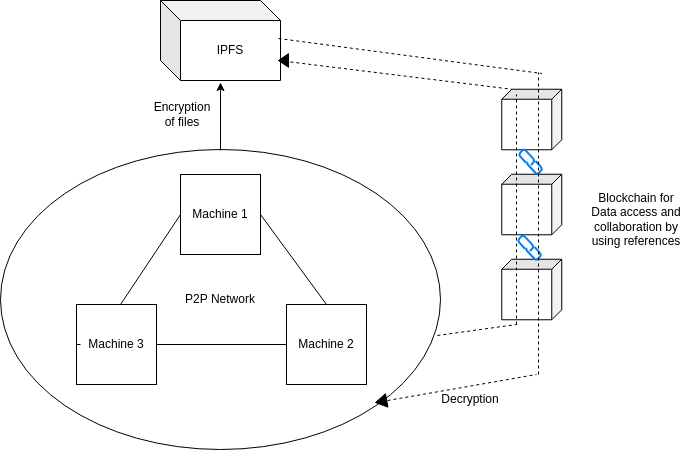
\includegraphics[width=14cm]{images/arch.png}
% \begin{center}
%     Proposed System Design
% \end{center}

\section{Dataset Description}

\noindent This research will be conducted using the HAM10000 ("Human Against Machine with 10000 training images") dataset \cite{tschandl2018ham10000}. This is a widely-used benchmark for dermatoscopic image classification, consisting of 10,015 multi-source dermatoscopic images of common pigmented skin lesions. The images are collected from different populations and modalities, representing a realistic clinical distribution. The dataset is classified into seven key diagnostic categories:

\begin{itemize}
    \item Actinic keratoses and intraepithelial carcinoma (akiec)

    \item Basal cell carcinoma (bcc)

    \item Benign keratosis-like lesions (bkl) (solar lentigines / seborrheic keratoses / lichen planus-like keratoses)

    \item Dermatofibroma (df)
 
    \item Melanoma (mel)

    \item Melanocytic nevi (nv)

    \item Vascular lesions (vasc) (angiomas, angiokeratomas, pyogenic granulomas and hemorrhage)
\end{itemize}

A significant challenge of this dataset is its severe class imbalance, with Melanocytic nevi (nv) comprising a majority of the samples. This imbalance necessitates the use of robust training strategies, such as weighted loss functions, class-aware sampling, and advanced data augmentation, to prevent the model from being biased towards the majority class. For our experiments, the dataset will be partitioned into training, validation, and testing sets with a standard 80-10-10 split, ensuring that the class distribution is stratified across all splits.
\section{Methodology}
The proposed methodology is a comprehensive three-phase pipeline, as detailed in previous chapters. Here we provide a structured overview:

\begin{enumerate}
    \item \textbf{Phase 1:} Self-Supervised Pre-training: A Vision Transformer (ViT-B/16) backbone will be pre-trained on the entire HAM10000 training set using the Momentum Contrast v3 (MoCo v3) framework. This will produce a set of weights that are highly adapted to the specific domain of dermatoscopic imagery.
    
    \item \textbf{Phase 2:} Teacher Model Training: The pre-trained backbone will be integrated into our novel Context-Aware Hierarchical Vision Transformer (CA-HVT). This teacher model will then be fine-tuned on the labeled training data in a fully supervised manner. The objective is to maximize diagnostic accuracy, creating an "expert" model that serves as the gold standard for knowledge distillation.
 
    \item \textbf{Phase 3:} Knowledge Distillation: The trained CA-HVT teacher model's knowledge will be transferred to a lightweight TinyViT student model. This will be accomplished using our proposed Attention-Guided Relational Knowledge Distillation (ARK-KD) framework. The student will be trained to mimic the teacher's logits, feature space geometry, and spatial attention patterns simultaneously.

    \item \textbf{Evaluation:} The final distilled student model will be rigorously evaluated on the held-out test set. We will report a comprehensive set of metrics, including overall accuracy, per-class F1-score, precision, recall, and balanced accuracy. We will also perform qualitative analysis using techniques like Grad-CAM to interpret the model's decision-making process.

\end{enumerate}
\section{Proposed Research Timeline}
\noindent The following table outlines the proposed timeline for the completion of this research thesis over a 12-month period.\\
    % \centering
    % 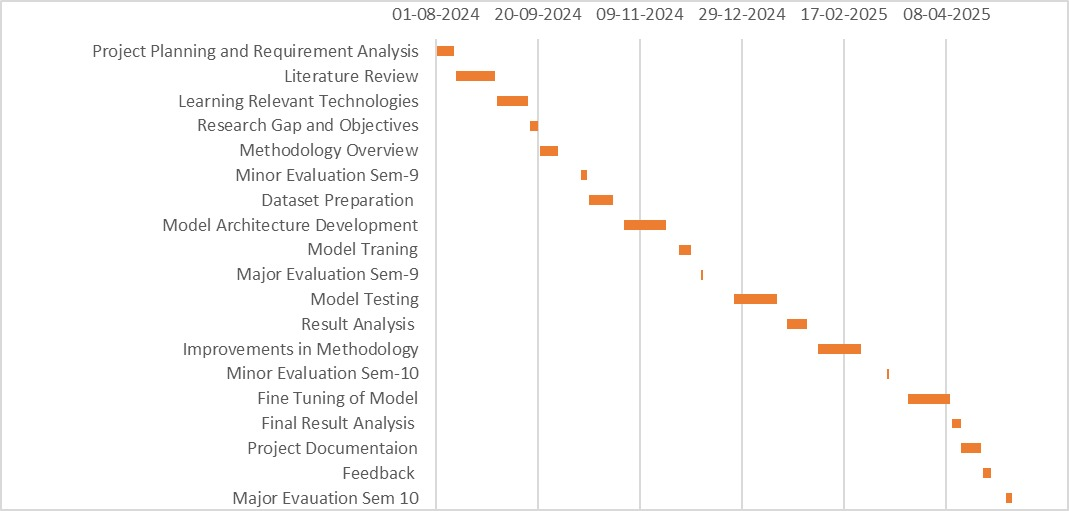
\includegraphics[width=16cm]{chapters/1/WhatsApp Image 2024-10-11 at 14.49.55.jpeg}



\begin{table}[h!]
\centering
\caption{Proposed Research Timeline}
\label{tab:gantt}
\renewcommand{\arraystretch}{1.4}
\begin{adjustbox}{max width=\textwidth}
\begin{tabular}{| p{6cm} | c | c | c | c | c | c |}
\hline
\textbf{Task} & \textbf{M 1-2} & \textbf{M 3-4} & \textbf{M 5-6} & \textbf{M 7-8} & \textbf{M 9-10} & \textbf{M 11-12} \\
\hline
1. Literature Review \& Finalizing Proposal & \cellcolor{gray!40} & & & & & \\
\hline
2. Data Preparation \& Pre-processing & \cellcolor{gray!40} & & & & & \\
\hline
3. Phase 1: SSL Pre-training & & \cellcolor{gray!40} & & & & \\
\hline
4. Phase 2: CA-HVT Teacher Implementation \& Training & & & \cellcolor{gray!40} & & & \\
\hline
5. Phase 3: ARK-KD Distillation Implementation \& Training & & & & \cellcolor{gray!40} & & \\
\hline
6. Model Evaluation and Results Analysis & & & & & \cellcolor{gray!40} & \\
\hline
7. Thesis Writing: Methodology \& Results Chapters & & & & \cellcolor{gray!40} & \cellcolor{gray!40} & \\
\hline
8. Thesis Writing: Introduction, Discussion \& Conclusion & & & & & & \cellcolor{gray!40} \\
\hline
9. Final Review and Thesis Submission & & & & & & \cellcolor{gray!40} \\
\hline
\end{tabular}
\end{adjustbox}
\end{table}

\label{chap:Future Direction}

% ---------------------------------------------


% --------- Uncomment for Model Architecture  and Methodology----------
% \chapter{Model Architecture}
% \vspace{-1cm}
% \noindent \rule{6.6in}{0.01in}
% % \section{Model Architecture}
% \noindent In this section we will discuss about the architecture of base and target model.
% \begin{enumerate}
\section{Base Model} 

\noindent We have used GroundedSAM as a base or foundation model; GroundedSAM is a combination of GroundingDINO\cite{GroundingDINO} and Segment Anything Model\cite{Segment} to recognize and segment objects in an image with a given input text caption. 
% \begin{enumerate}
\subsection{Grounding DINO}
\noindent GroundingDINO is a zero-shot object detector. Most object identification models are developed to recognize a small set of predefined classes. The primary issue with this is that it needs to be more flexible. Whenever you wish to increase or modify the list of recognizable objects, you must gather data, label it, and retrain the model. Of course, doing this takes time and money. New object detection is made feasible without re-training a model thanks to zero-shot detectors like GroundinDINO. You must alter the prompt to get the model to recognize the objects you describe.

Grounding DINO combines the concepts published in the DINO\cite{dino} and GLIP papers\cite{glip}. DINO is an object detection method that is based on transformers. It gives state-of-the-art performance for object detection along with end-to-end optimization. At the same time, GLIP is more concerned with phrase grounding. This task tries to match phrases or words from a given text with equivalent visual elements in an image or video to connect textual descriptions to their corresponding visual representations.

It uses a text backbone like BERT to extract the text features and an Image backbone like Swin Transformer to extract Multiscale image features. Following the extraction of basic image and text features, the features are passed into the feature enhancer \ref{fig:DINO}, which contains several layers to combine features from several inputs. Different strategies are used to improve the text and image features.
A language-guided query selection module \ref{fig:DINO} is created to choose features more pertinent to the input text as decoder queries to exploit the input text for effectively guiding object detection. A cross-modality decoder is designed to merge the properties of text and visual modality properties. The model excels in numerous real-world tasks because it can recognize objects outside its training set and process language and visual content\cite{Ahmad_2023}.
\begin{figure}[h]
\centering
	\includegraphics*[width = 13cm]{images/DINO.png}
	 \caption{Grounding DINO overall Model}\cite{GroundingDINO}
	\label{fig:DINO}
\end{figure}
% \begin{center}
% 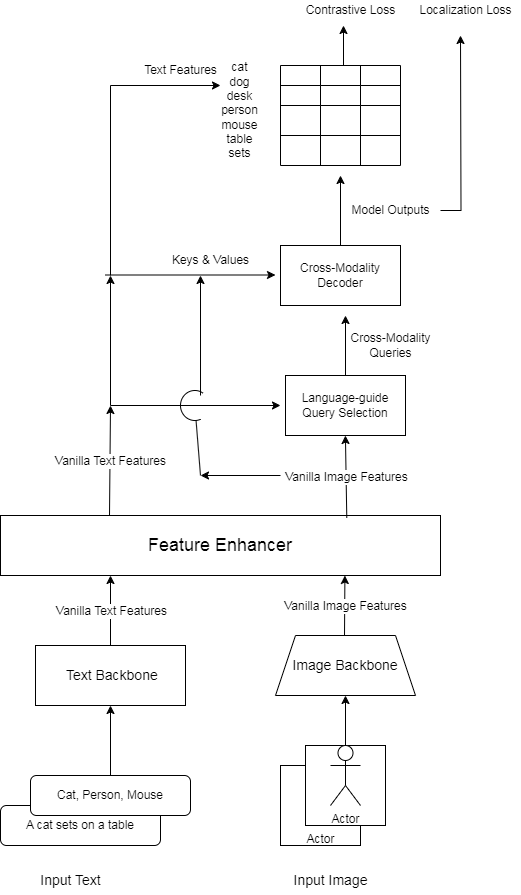
\includegraphics[width=13cm]{images/DINO.png}
% \end{center}

% \item Segment Anything Model:
\subsection{Segment Anything Model}

\noindent This model proposes a new dataset, model, and task for image segmentation.
The Segment Anything project builds a foundational or base model for image segmentation by using prompt engineering that solves various segmentation problems on new data.
% \begin{wrapfigure}{i}{}
%     \centering
%     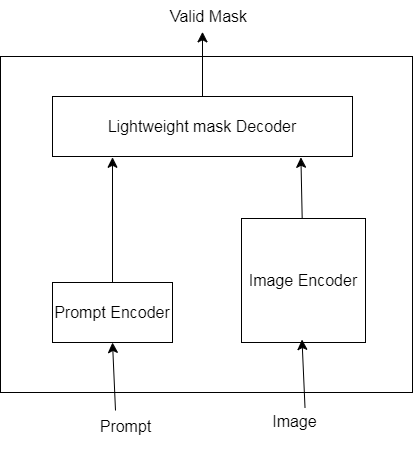
\includegraphics[width= 13cm]{images/segment.png}
%     \caption{Segment Anything Model}
%     \label{fig:segment}
% \end{wrapfigure}
% \begin{figure}[h]
% \centering
% 	\includegraphics*[width = 13cm]{images/segment.png}
% 	 \caption{Segment Anything Model}
% 	\label{fig:segment}
% \end{figure}

% \begin{center}
% 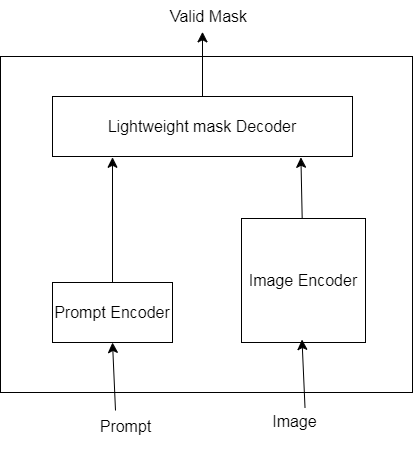
\includegraphics[width=8cm]{images/segment.png}
% \end{center}

The project's main elements are:
\begin{itemize}
    \item Task: A promptable segmentation task aims to return a valid segmentation mask for a given input prompt. Here valid means model should produce the most probable mask in the case of unclarity in the prompts provided. The segmentation prompt can be in the form of text, box, mask, or image.
    \item Model: The segment anything model consists of a lightweight mask decoder, image encoder, and prompt encoder \ref{fig:segment}. The mask decoder combines the information from the image encoder and prompt encoder to give a valid segmentation mask.

    \item Data: The required dataset is collected using a data engine. The Data Engine has three phases. SAM helps annotators generate the masks in the first stage. In the second stage, SAM automatically generates masks, and annotators concentrate on annotating the remaining objects. In the third stage, SAM is provided with a regular grid of points as input and generates the image masks.
\end{itemize}
The model's performance demonstrates that it can be a foundational model for image segmentation.
\begin{figure}[H]
\centering
	\includegraphics*[width = 7cm]{images/segment.png}
	 \caption{Segment Anything Model}\cite{Segment}
	\label{fig:segment}
\end{figure}
% \end{enumerate}

\section{Target Model} 

\noindent We are using YOLOv8 as a target model for surface floating object detection.

    \subsection{Characteristics}
    \noindent In YOLOv8, several features are to be prioritized. Object detection accuracy is increased by YOLOv8 compared to its predecessors by implementing new approaches and optimizations. It offers higher accuracy and faster inference speeds than existing object identification algorithms. It supports many backbones, including EfficientNet, ResNet, and CSPDarknet, allowing users to select the model suitable for their particular use case. Using adaptive training, YOLOv8 improves model performance by optimizing the learning rate and balancing the loss function during training. To increase the robustness and generalizability of the model, YOLOv8 uses sophisticated data augmentation techniques, including MixUp and CutMix. YOLOv8's architecture is adaptable, enabling users to quickly change the model's structure and parameters to meet their needs. It offers pre-trained models for convenient use and transfers learning across various datasets.

    \subsection{Architecture}
    
    \noindent The YOLOv8 architecture expands on earlier iterations of the YOLO algorithms. Because YOLO operates on the whole image simultaneously, it is rapid and effective. This is where the YOLOv8 differs from other object detection algorithms, which take a sliding window method that is expensive in computing. The convolutional neural network used by YOLOv8 comprises two primary sections the head and the backbone. The foundation of YOLOv8 is a modified version of the CSPDarknet53 architecture. Fifty-three convolutional layers make up this design, using cross-stage partial connections to enhance information transfer between the various layers. The head consists of many convolutional layers and fully linked layers. These layers are responsible for calculating bounding boxes, objectness scores, and class probabilities for the objects detected in an image. In Yolov8, bounding box predictions are made pixel-wise. An anchor-free detection head is introduced for this purpose. With the help of anchor-free detection \ref{fig:anchor}, an object detection model can predict the center of the object instead of the offset from the anchor box. The capability of YOLOv8 to carry out multi-scaled object identification is another crucial feature. The model uses a feature pyramid network to find items in an image with different sizes and scales.

\begin{figure}[H]
\centering
	\includegraphics*[width = 8cm]{images/Anchor-free.png}
	 \caption{Anchor Free Detection}
	\label{fig:anchor}
\end{figure}
% \begin{center}
% 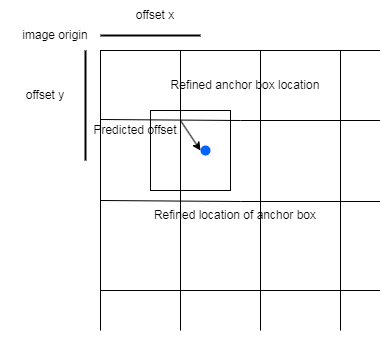
\includegraphics[width=10cm]{images/Anchor-free.png}
% \end{center}

\noindent Feature Pyramid Network (FPN)\cite{fpn} is a deep learning architecture designed to address the problem of object detection and recognition in images at multiple scales. In CNN architectures, the higher layers typically capture semantic information but lose spatial resolution, while lower layers capture finer spatial details but lack high-level semantics \ref{fig:variation}. FPN bridges this gap by constructing a multi-scale feature representation of the input image. FPN starts with a standard CNN for feature extraction from the input image. The backbone CNN processes the input image through several layers to obtain feature maps at different scales. These feature maps have decreasing spatial resolution but increasing semantic information as we move higher in the network \ref{fig:variation}.\\

\begin{figure}[H]
\centering
	\includegraphics*[width = 10cm]{images/variation.png}
	 \caption{Feature Extraction in FPN}
	\label{fig:variation}
\end{figure}
% \begin{center}
% 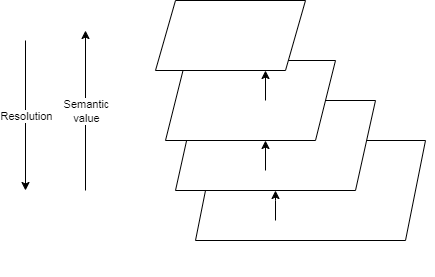
\includegraphics[width=10cm]{images/variation.png}
% \end{center}

\noindent FPN introduces a top-down pathway to upsample the feature maps and recover the lost spatial resolution. This is achieved by applying upsampling or interpolation on the higher-level feature maps. To combine the bottom-up and top-down pathways, FPN introduces lateral connections. These connections fuse the high-resolution features from the bottom-up pathway with the upsampled features from the top-down pathway \ref{fig:bottom}. The final output of FPN is a set of feature maps at multiple scales, each capturing different semantic and spatial information levels \ref{fig:bottom}.
\\\\

\begin{figure}[H]
\centering
	\includegraphics*[width = 12cm]{images/FPN.png}
	 \caption{Feature Pyramid Network}\cite{fpn}
	\label{fig:FPN}
\end{figure}
% \begin{center}
% 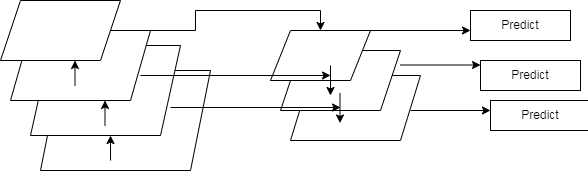
\includegraphics[width=12cm]{images/FPN.png}
% \end{center}

\begin{figure}[H]
\centering
	\includegraphics*[width = 13cm]{images/Bottom-up.png}
	 \caption{Bottom-up and Top-Down Pathway}\cite{fpn}
	\label{fig:bottom}
\end{figure}
% \begin{center}
% 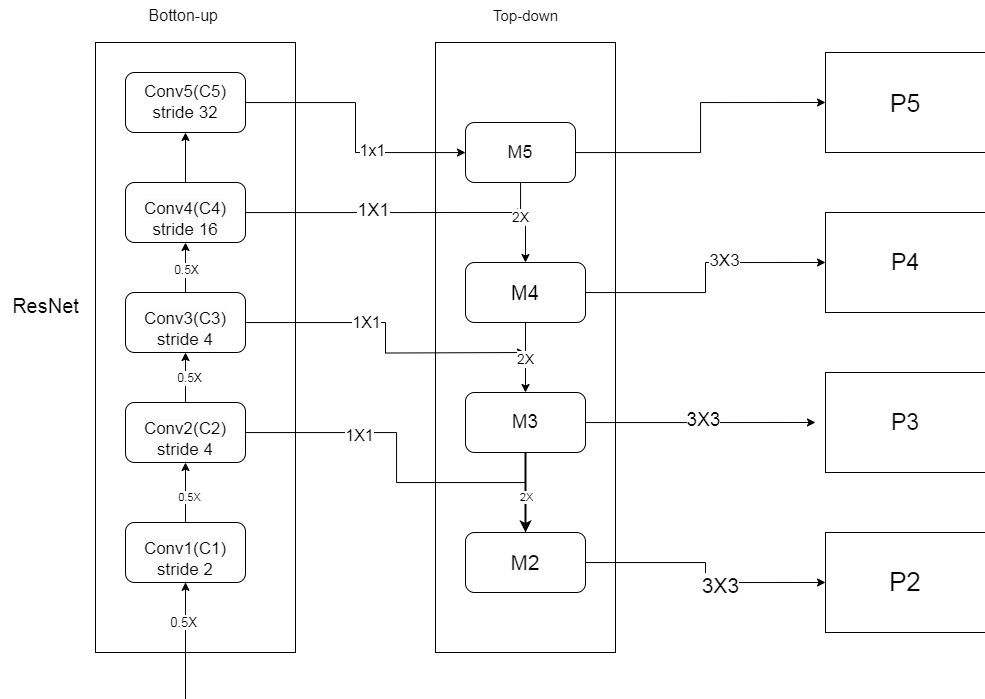
\includegraphics[width=12cm]{images/Bottom-up.png}
% \end{center}
% \end{enumerate}

\vspace{\baselineskip}

\noindent The use of FPN in object detection tasks has shown significant improvements in accuracy, especially when dealing with objects of different sizes within an image. By leveraging multiple-scale information, FPN enables the network to handle large and small objects better, improving object detection performance.


% \end{enumerate}
% \section{Thesis Objective}

%  \begin{enumerate}
%     \item To study and develop a solution for predicting the description of the images in real-time with good accuracy.
%     \item To further modify the existing models on image description generation with new modifications to reduce the complexity and training time of the proposed model.
%     \item To further automate the process of selecting the encoder for the neural network architecture to generate the description for the image.
%     \item To develop a native mobile application for fetching the description given in the image.
% \end{enumerate}
\label{chap:problem_statement}

% \chapter{Methodology and Progress}
% \vspace{-1cm}
% \noindent \rule{6.6in}{0.01in}
% \clearpage

\section{Methodology}

\noindent
\begin{enumerate}
    \item Dataset: 
    Common data sets cannot be trained to recognize the objects on the water's surface.  We have used the Flow Dataset for floating waste objects, this dataset contains 2000 images with 5271 floating wastes like plastic bottles and drinking cans. We have done a balanced Train-Validate-Test Split. Along with images dataset also contains 200 sequence videos for training. The interval of the video varies from several seconds to a minute. Each video contains almost 1-8 floating waste instances. 	We have converted this raw video into images by extracting the frames. Our dataset contains more small objects, which makes it challenging for detection.

\item Base Model Architecture Selection:
In this project, as we are using the concept of distillation, we require two models the first one is the base model, and the other one is the target model. As annotating data is very time and money-consuming, We are using GroundedSAM as a base model, automatically annotating the images we have taken from the FloW dataset. GorundedSAM uses grounding DINO to detect and label the images and uses the Segment Anything Model to generate the masks of images. So by combining the power of DINO, GLIP, and SAM, we can automatically annotate our data.


\item Dataset preparation:
The base model GroundedSAM will take raw images and videos as input along with the proper ontology to annotate the data to produce the auto-label dataset automatically. This dataset can be used to train the target YOLOv8 model.
As we need to compare the results of distillation from GroundedSAM to YOLOv8 and the performance of training YOLOv8 without distillation, We preprocessed the dataset by resizing images to a consistent resolution, normalizing pixel values, and converting annotations into the YOLOv8-compatible format using Roboflow tool. \textbf{make each of these bullets as just paragraphs with headlines in bold and add citations and references wherever required}


\item Target Model Architecture Selection:
For the target model, We have chosen the YOLOv8 for developing the floating object detection model. YOLOv8 (You Only Look Once v8) is a state-of-the-art object detection model developed by Ultralytics. It is a real-time object detection model that can achieve high accuracy and speed. It is an advanced variant in the YOLO family. YOLOv8 is also a good choice for floating object detection because it is specifically designed to detect objects at different scales. This is important for floating object detection, as floating objects can vary significantly in size. YOLOv8's ability to detect objects at different scales makes it more likely to accurately detect floating objects in images and videos.


\item Distillation:
Although effective, foundation models like GroundedSAM include limitations such as high GPU computation requirements, slow real-time performance, and restricted accessibility. These restrictions prevent its application in low-compute environments, such as edge devices, inhibit the development of original intellectual property, and prevent cost-effective use. Although foundation models have a wealth of information across many fields, many real-world applications of AI demand an in-depth understanding of specific fields. Distillation offers a way to utilize the power of expansive models without direct deployment. It transfers the knowledge of the expensive vase model to the target model without affecting efficiency and accuracy to get a fast and deployment-ready model\cite{Distill}. In this project, we are transferring the knowledge of object detection from GroundedSAM to the YOLOv8 model with the help of the AutoDistill library.


\item Model Training:

The target model YOLOv8 takes the auto-labeled data produced by the GroundedSAM and gives the deployment-ready model for floating waste detection. We have trained the YOLOv8 on both datasets, the one automatically labeled by the groundedSAM and the one labeled manually using the labeling tool.
The cosine Annealing method is used in the training phase of YOLOv8.
Cosine annealing is a learning rate decay strategy that uses a cosine function to decrease the learning rate gradually over time. The learning rate is initialized at a high value and then drops to a lower value throughout training. It helps to produce good results. The deep learning framework is TensorFlow, GPU is Tesla 4, during training, the batch size is set to 16, the training epoch is set to 100, and the learning rate is 0.001. 

\item  
Model Testing: 
The output of the trained model gives us the distilled model, which successfully recognizes floating waste objects in various images. These results show that distillation from GroundedSAM to YOLOv8 is a powerful floating object detection tool model that is accurate, fast, and can detect a wide variety of objects.
\\

\end{enumerate}

\section{Task Completed}
\begin{enumerate}
    \item Image Dataset Preparation: 
    Downloaded the raw images and videos of floating waste objects from the FloW dataset, ensuring that most objects are small. We have split the videos into images by saving the 15th frame from each video. We have also kept videos for evaluating the model.

\item Select the model for floating waste detection:
We have selected the GroundedSAM as a base model and YOLOv8 as a target model.


\item Setup Python environment and Install dependencies: We have set up the GPU environment and installed the required dependencies. As we are using the concept of distillation, we have installed the Autodistill library. And for the base and target models, we have installed Autodistill packages that are required for our chosen models.


\item Define Ontology: 
We have used CaptionOntology. It prompts a Base Model with text captions and maps them to class names. We have defined the Ontology to detect the waste floating on the water's surface, basically plastic bottles and drink cans.


\item Autolabel the images:
We have initialized the base model GroundedSAM with unlabeled input data and ontology to convert into the annotated dataset. As base models are very slow but efficient, take took 2 hours of time time to annotate the data.


\item Display sample of dataset:
The dataset is the result of the GroudedSAM model. This dataset will be used to train YOLOv8. The dataset contains automatically labeled images. We are displaying a sample of data to look at the model's performance.

\item Distillation from base to target model:
We have distilled the knowledge from the base model groundedeSAM to YOLOv8. Now YOLOv8 will consume the auto-labeled data and give a fast and real-time distilled model for deployment.

\item Training of model: 
We have trained the YOLOv8 on auto-labeled and manually annotated data. So that we can compare the results of the training with or without knowledge distillation.

\item Evaluating and Testing the Model:
We have evaluated and tested the model on the FloW dataset.

\end{enumerate}

\section{Experiment and Result Analysis}
This section discusses the results of the project.
% \noindent\\
    % \centering
\begin{enumerate}
\item Sample of data:
\ref{fig:Data} shows the sample from the dataset used as input for the groundedSAM model.

\item Data sample generated by GroundedSAM:
The following \ref{fig:Dataset} shows the outstanding result of GroundedSAM for automatically Annotating the data. It outputs the masks of waste objects from the images.

\begin{figure}[H]
\centering
	\includegraphics*[height=10cm, width = 10cm]{images/Data-Sample.png}
	 \caption{Data Sample}
	\label{fig:Data}
\end{figure}

 \item Training Result:
\ref{fig:t-auto} shows the result of the training YOLOv8 on the auto-labeled dataset generated by the GroundedSAM. This is the result when we just give images and text prompts to the GroundedSAM model and then distill the knowledge from the base model to the target model. It gives 0.741 mAP50. 
\ref{fig:t} shows the result of the training YOLOv8 on the annotated FloW dataset. This is the result when we are giving annotated FloW dataset to YOLOv8. We have trained the YOLOv8 model for 100 epochs from scratch for this custom dataset for a batch size of 16. It gives 0.925 mAP50.
The training results are summarized in the \ref{table:training-1}
\newline

\item Evaluation Result: We have evaluated the distilled model on the 400 validating images. \ref{fig:eval} shows the result of one batch with size 16.\newline 
\begin{figure}[H]
\centering
	\includegraphics*[height=10cm, width = 10cm]{images/Data-Sample-generated-GroundedSAM.png}
	 \caption{Data Sample generated by GroundedSAM}
	\label{fig:Dataset}
\end{figure}


\item Test Results:
While testing, the model clearly shows that it can detect floating waste objects in complex environment situations \ref{fig:test} like reflections and excessive light. The distilled model has given state-of-the-art performance for detecting floating waste objects by taking prompts and images as input. The results are also compared with other models in table \ref{table:training-1} and table \ref{table:training-3}. We have also compared the Speed per image and FPS for YOLOv8 and DistilledFloatNet in table \ref{table:training-2}
% 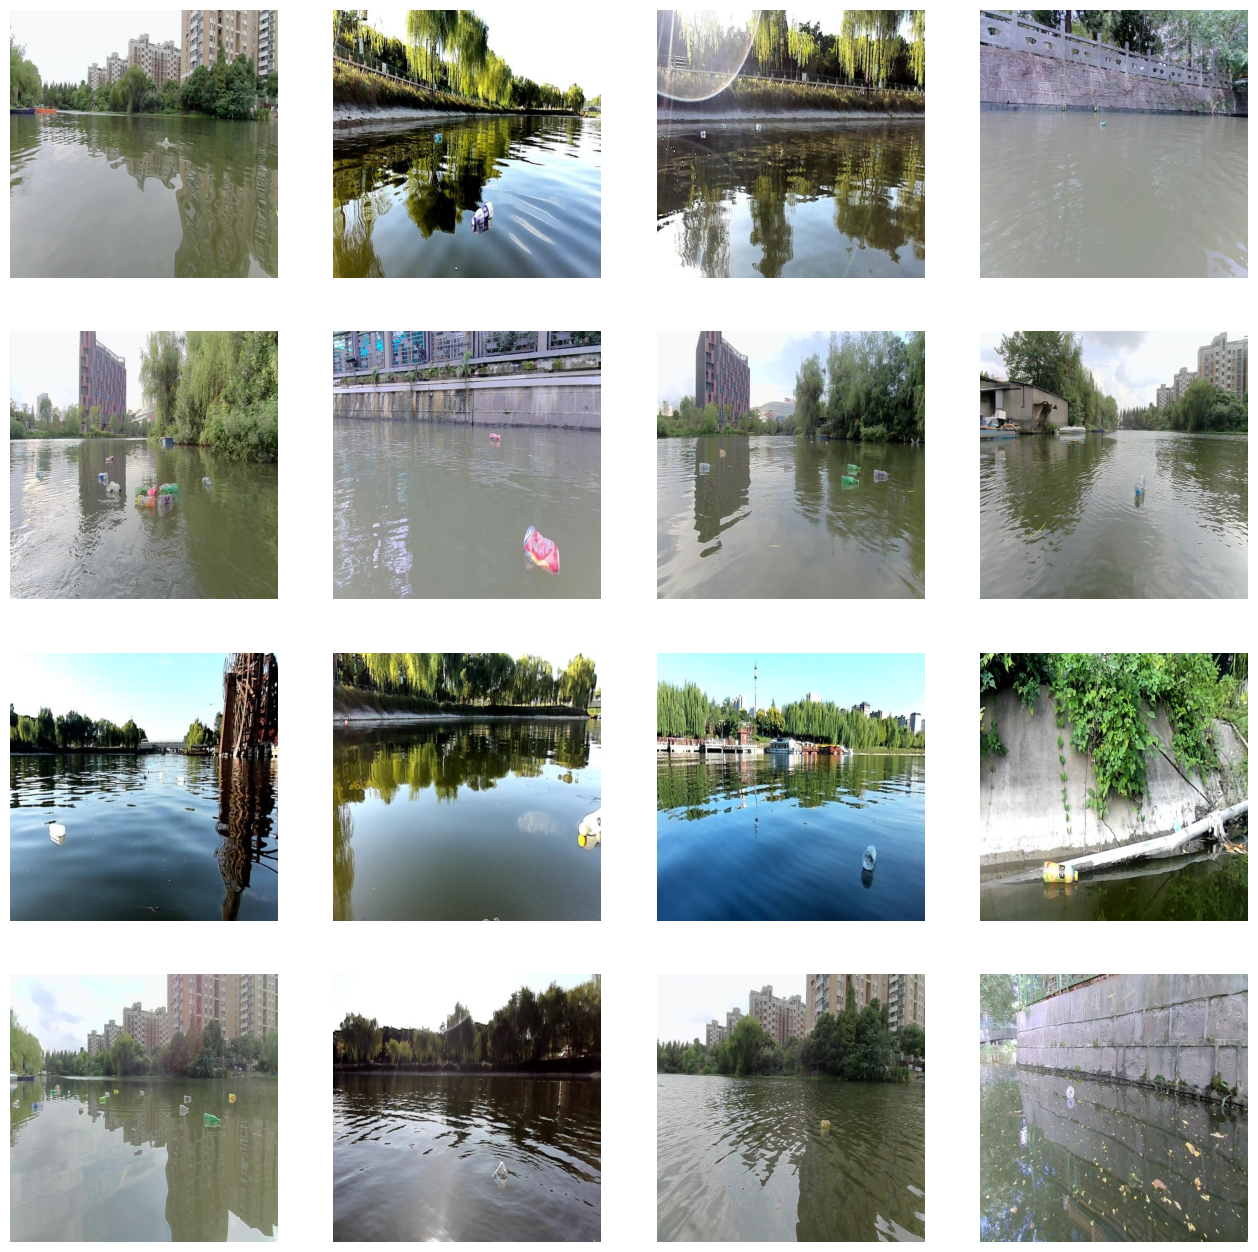
\includegraphics[width=14cm]{images/Data-Sample.png}
% \begin{center}
%     Fig(7) Data Sample
% \end{center}
%  \begin{table}
%     \centering
   
%    \begin{tabular}{ | m{8em}| m{6em} | m{5em} | m{6em} | m{7em}|} 
%         \hline
%         \textbf{Model} & \textbf{Precision\%} & \textbf{Recall\%} & \textbf{mAP50\%} & \textbf{mAP50-95\%} \\
%         \hline
%         GroundedSAM \newline and YOLOv8 \newline using Distillation & 69.9 & 69.5 & 74.1 & 55.4 \\
%         \hline
%         YOLOv8 \newline without\newline using Distillation & 90.9 & 88.5 & 92.5 & 52.2 \\
%         \hline
%     \end{tabular}
%     \centering
%      \caption{Training Results}
%      \label{table:1}
% \end{table}   

\begin{table}
    \centering
    \label{tab:my_label}
\begin{tabular}{lccccr}
\hline \multicolumn{1}{c}{\textbf{Model}} & \textbf{Precision\%} & \textbf{Recall\%} & \textbf{mAP50\%} & \textbf{mAP50-95\%}\\
\hline 
DistilledFloatNet & 69.9 & 69.5 & 74.1 & 55.4\\
YOLOv8 & 90.9  & 88.5 & 92.5 & 52.2 \\
\hline
\end{tabular}
\caption{Training Results}
\label{table:training-1}
\end{table}

% 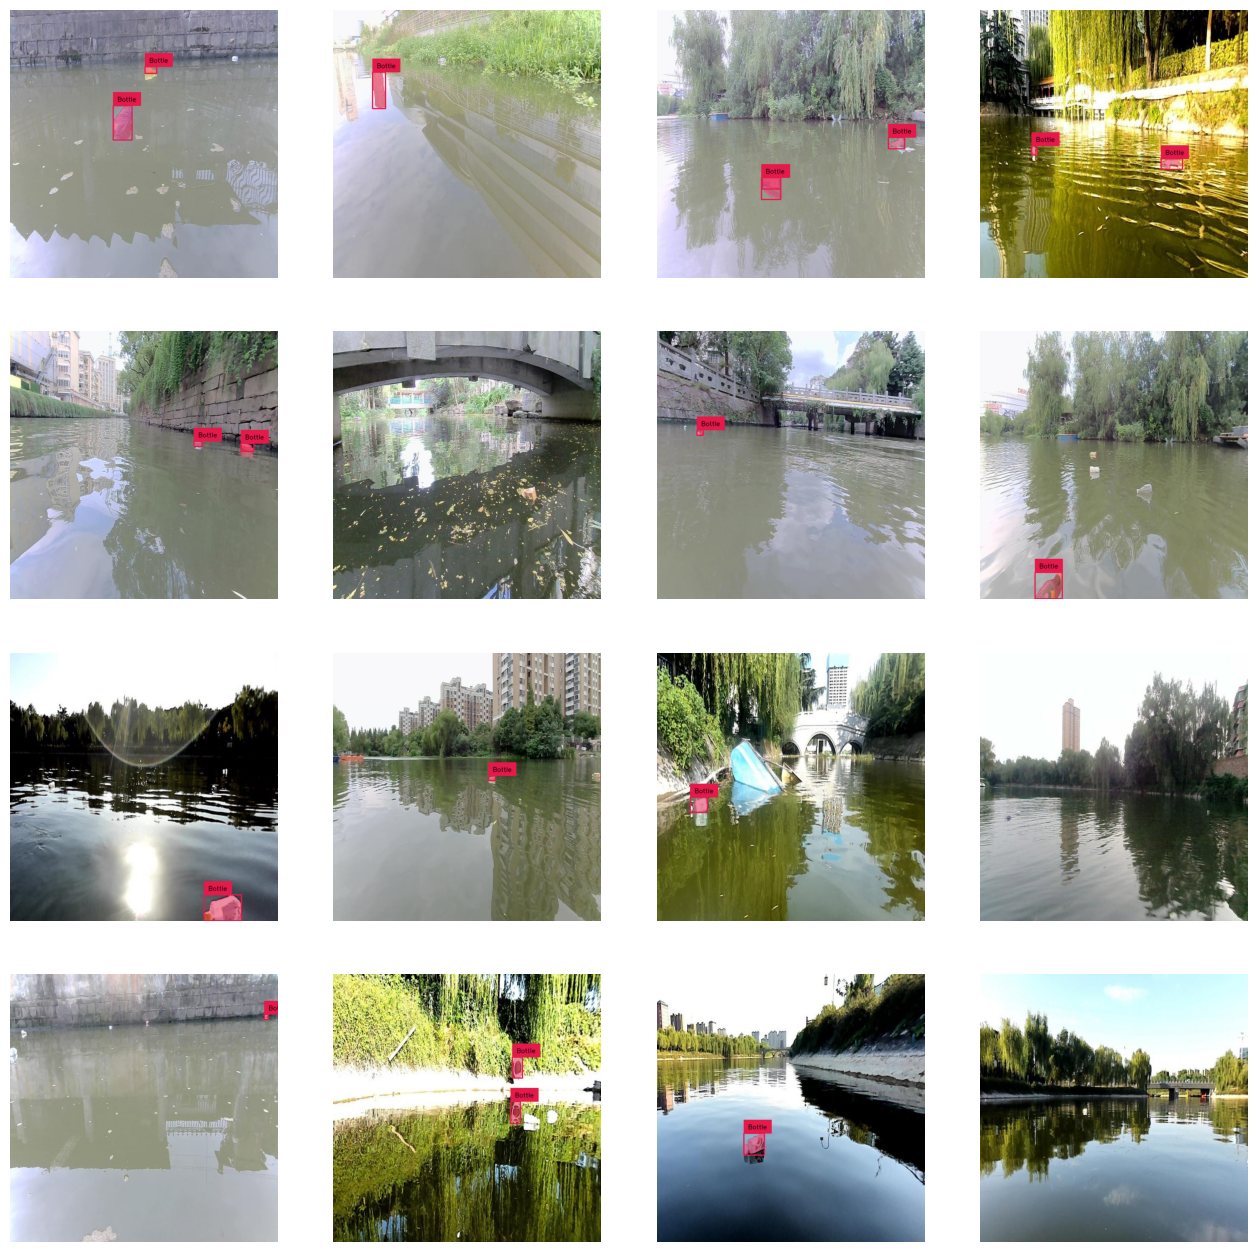
\includegraphics[width=14cm]{images/Data-Sample-generated-GroundedSAM.png}
% \begin{center}
%     Fig(8) Data Sample generated by GroundedSAM
% \end{center}
\vspace{\baselineskip}
\vspace{\baselineskip}

\begin{figure}[H]
\centering
	\includegraphics*[width = 14cm]{images/training-result-with-distillation.png}
	 \caption{Training result with distillation}
	\label{fig:t-auto}
\end{figure}

% 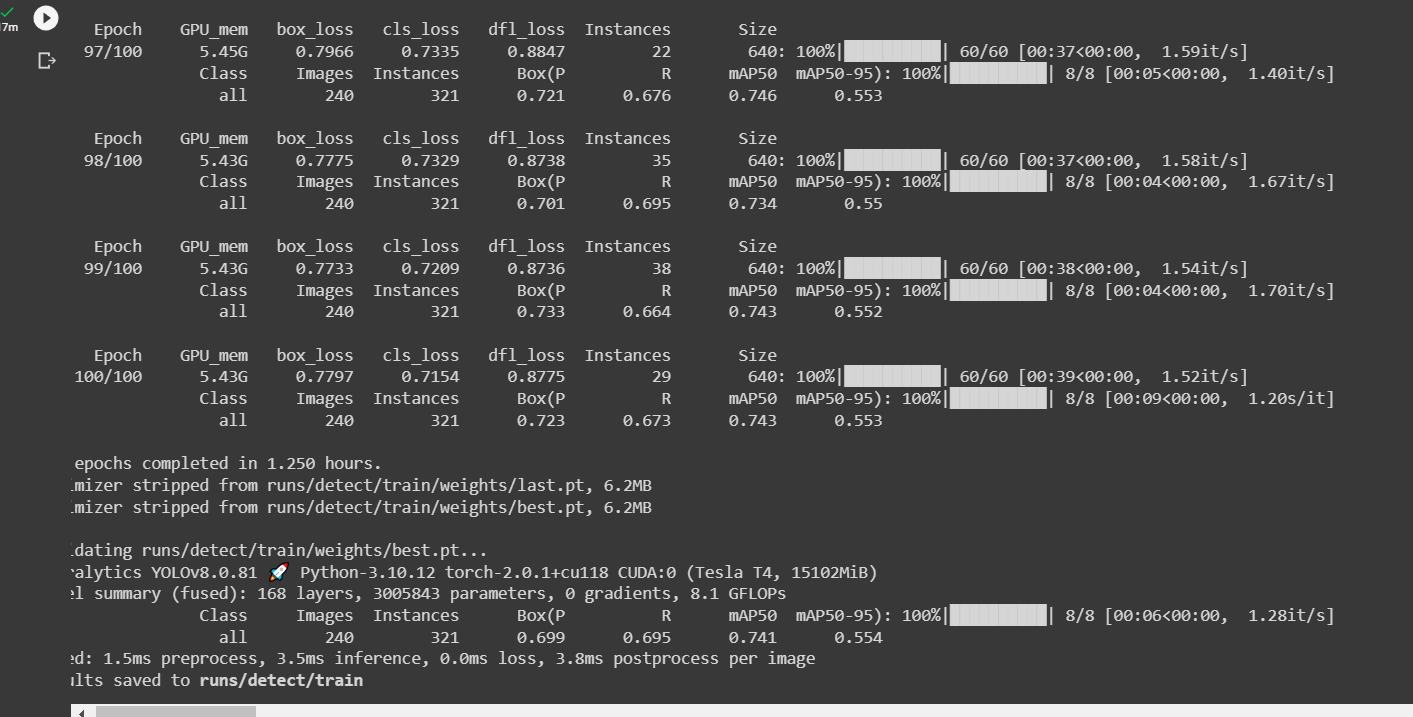
\includegraphics[width=14cm]{images/training-result-with-distillation.png}
% \begin{center}
%     Fig(9) Training result with distillation
% \end{center}
\vspace{\baselineskip}
\vspace{\baselineskip}


\begin{figure}[H]
\centering
	\includegraphics*[width = 14cm]{images/training-result-without-distillation.png}
	 \caption{Training result without distillation}
	\label{fig:t}
\end{figure}

% 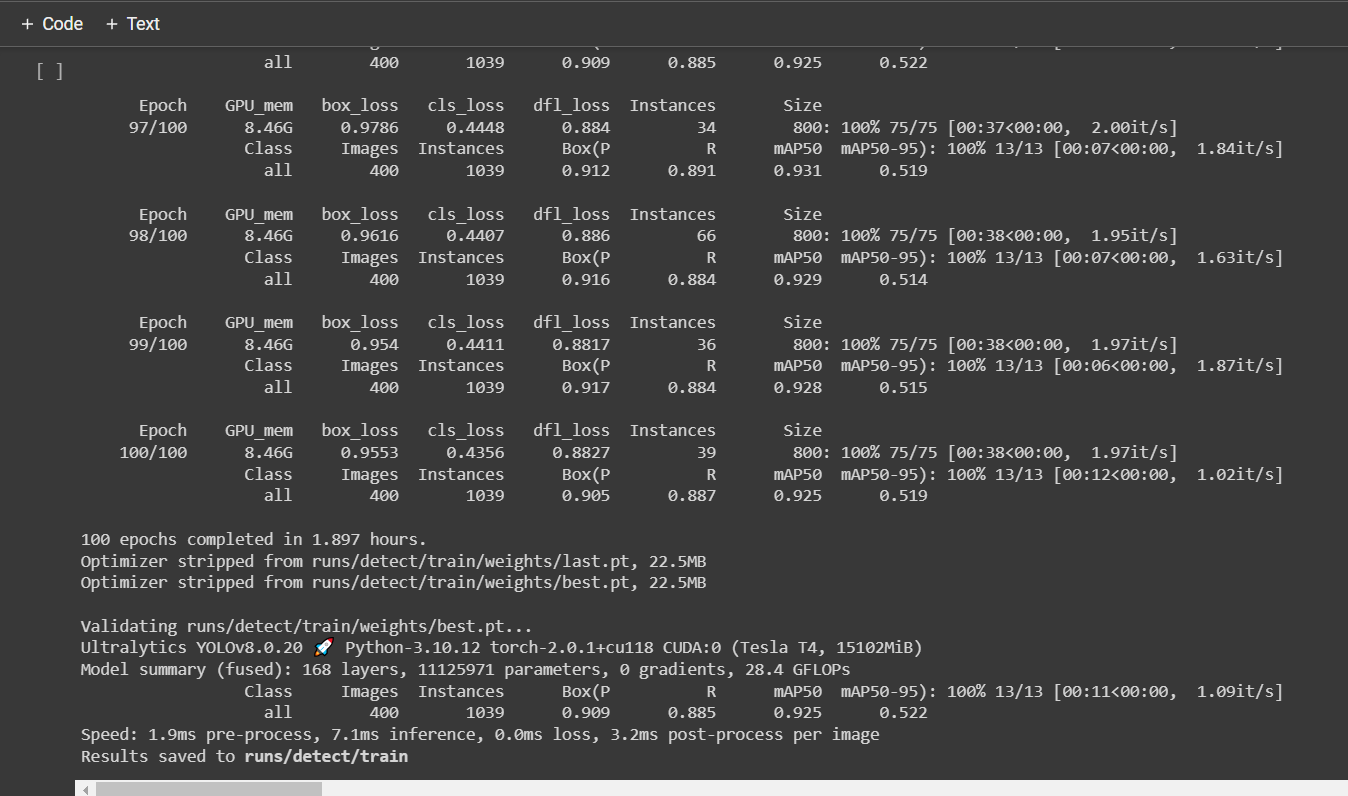
\includegraphics[width=14cm]{images/training-result-without-distillation.png}
% \begin{center}
%     Fig(10) Training result without distillation
% \end{center}
\begin{table}[H]
    \centering
    \label{table:training-2}
\begin{tabular}{lcr}
\hline \multicolumn{1}{c}{Model} & Dataset & mAP50-95\\
\hline 
DSSD & $FloW$ & 27.5 \%\\
RetinaNet & $FloW$  & 24.9 \% \\
YOLO-v3 & $FloW $ & 12.8 \% \\
Faster R-CNN & $FloW $ & 18.4 \% \\
FPN & $FloW $ & 33.4 \% \\
Cascade R-CNN & $FloW $ & 43.4 \% \\
\textbf{YOLOv8} & $\textbf{FloW} $ & \textbf{55.2\%}\\
\textbf{DistilledFloatNet} & $\textbf{FloW}$ & \textbf{55.4 \% }\\
\hline
\end{tabular}
\caption{Comparison with other Models}
\end{table}

\begin{table}[H]
    \centering
   
\begin{tabular}{lccccr}
\hline \multicolumn{1}{c}{Model} & Pre-process & Inference & Post-process & FPS\\
\hline 
YOLOv8 & 0.4ms & 11.9ms & 5.2ms & 57.14\\
DistilledFloatNet & 0.7ms  & 10.0ms & 2.0ms & 78.74 \\
\hline
\end{tabular}
\caption{Speed per image and FPS}
 \label{table:training-2}
\end{table}

\begin{figure}[H]
\centering
	\includegraphics*[height=10cm,width = 10cm]{images/Evaluation_image.png}
	 \caption{Data Evaluation Result}
	\label{fig:eval}
\end{figure}



% \begin{figure}[H]
% \centering
% 	\includegraphics*[height = 9cm, width = 10cm]{images/test-img-1.png}
% 	 \caption{Test Image 1}
% 	\label{fig:test1}
% \end{figure}

% \begin{figure}[H]
% \centering
% 	\includegraphics*[height = 9cm, width = 10cm]{images/test-image-2.png}
% 	 \caption{Test Image 2}
% 	\label{fig:test2}
% \end{figure}

% \begin{center}
% 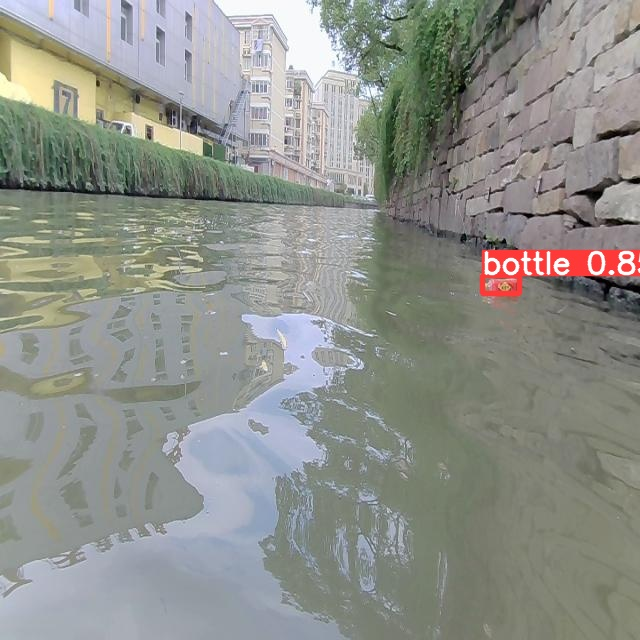
\includegraphics[width=10cm]{images/test-img-1.png}
% \begin{center}
%     Fig(12) Test Image 1
% \end{center}
% \end{center}

% \begin{center}
% 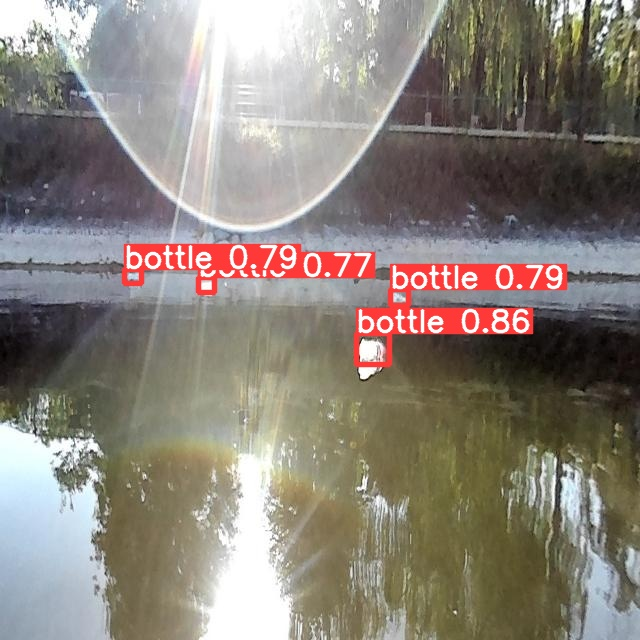
\includegraphics[width=10cm]{images/test-image-2.png}
% \begin{center}
%     Fig(12) Test Image 2
% \end{center}
% \end{center}

\item Loss Functions:
The loss functions are used to train the YOLOv8 model. For Bounding-Box loss, YOLOv8 uses the CIoU and DFL loss functions and BCE for class loss. These losses have increased object identification performance, especially with small objects. The model is trained to minimize the loss function. The loss functions can be used to analyze the performance of the YOLOv8 model. The lower the loss function, the better the model is performing. The loss functions can also identify areas where the model performs poorly. We have Monitored the loss functions during training in \ref{fig:r1} and \ref{fig:r2}: 
\begin{enumerate}
    \item The train/box-loss curve is a decreasing curve. This means that the box loss decreases as the model trains. A decreasing box loss indicates that the model is learning to predict the bounding boxes more accurately.
    \item The train/cls-loss curve is decreasing curve. This means that the cls-loss falls as the model trains. A decreasing cls-loss indicates that the model is learning to predict the classes more accurately.
    \item The dfl-loss curve is a decreasing curve. This means that the dfl-loss decreases as the model trains. A decreasing dfl-loss indicates that the model is learning to handle class imbalance better.
    \item The val/box-loss curve is a decreasing curve. This means that the val-box-loss decreases as the model validates. A decreasing val-box-loss indicates that the model is learning to predict the bounding boxes more accurately.
    \item The recall curve is an increasing curve. This means that the recall increases as the model trains. An increasing recall indicates that the model is becoming more confident in its predictions. This is because the model is learning to avoid false negatives.
    \item The val/cls-loss curve is a decreasing curve. This means that the val-cls-loss decreases as the model validates. A decreasing val-cls-loss indicates that the model is learning to predict the classes more accurately.
    \item The val/dfl-loss curve is a decreasing curve. This means that the val-dfl-loss decreases as the model validates. A decreasing val-dfl-loss indicates that the model is learning to handle class imbalance better.

\end{enumerate}
\textbf{what are the limitations and where its failing}


\begin{figure}[H]
\centering
	\includegraphics*[width = 14cm]{images/loss-function-distillation.png}
	 \caption{Result with Distillation}
	\label{fig:r1}
\end{figure}

\begin{figure}[H]
\centering
	\includegraphics*[width = 14cm]{images/loss-function-without-distillation.png}
	 \caption{Result without Distillation}
	\label{fig:r2}
\end{figure}

% 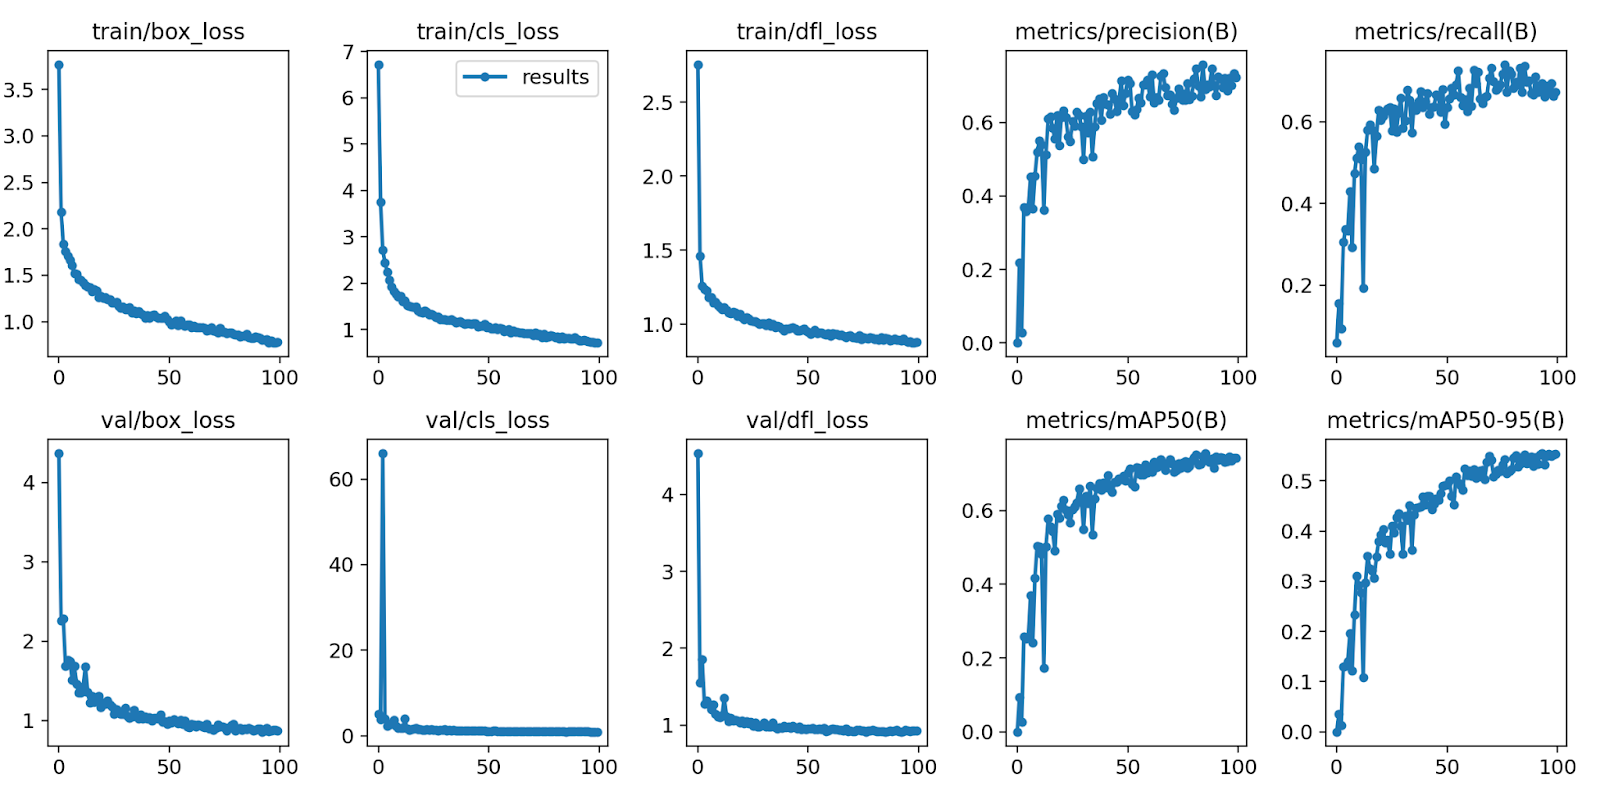
\includegraphics[width=14cm]{images/loss-function-distillation.png}
% \begin{center}
%     Fig(13) Result without Distillation
% \end{center}

% 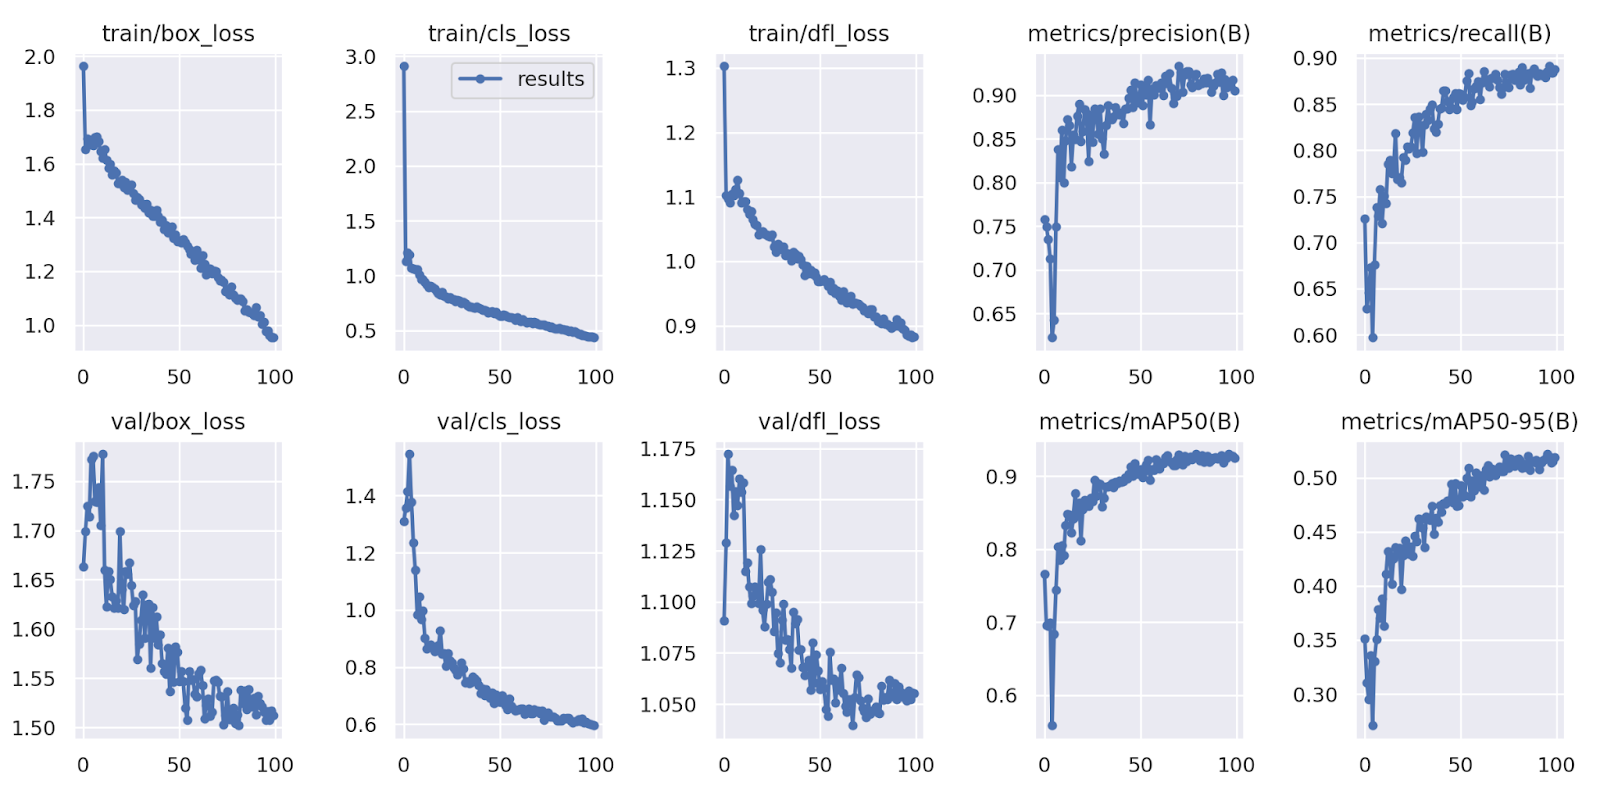
\includegraphics[width=14cm]{images/loss-function-without-distillation.png}
% \begin{center}
%     Fig(14) Result without Distillation
% \end{center}


% \documentclass{article}
% \usepackage{graphicx}
% \usepackage{subcaption}

% \begin{document}

% \begin{figure}[ht]
%   \subcaptionbox*{First subfigure}[.45]{%
%     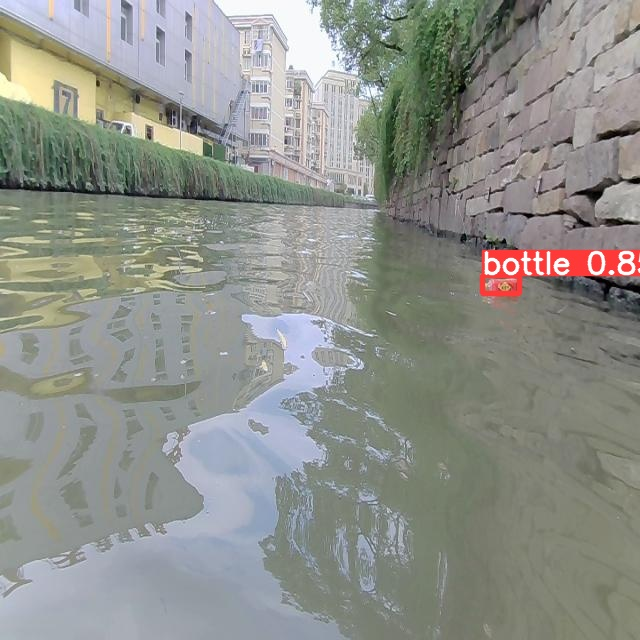
\includegraphics[width=5cm]{images/test-img-1.png}%
%   }%
%   \hfill
%   \subcaptionbox*{Second subfigure}[.45]{%
%     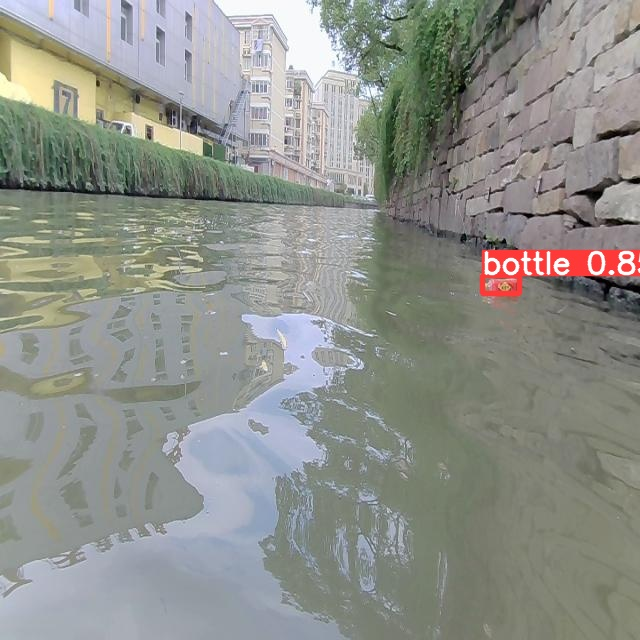
\includegraphics[width=5cm]{images/test-img-1.png}%
%   }
%   \caption{Two images}
% \end{figure}


% \end{document}

\end{enumerate}
\begin{table}[H]
    \centering
 
\begin{tabular}{lccr}
\hline \multicolumn{1}{c}{Model} & Dataset & mAP50-95 & FPS\\
\hline DSSD & $FloW $ & 27.5 \% & 28.6\\
RetinaNet & $FloW $  & 24.9 \% & 7.6\\
YOLO-v3 & $FloW $ & 12.8 \% & 23.2\\
Faster R-CNN & $FloW $ & 18.4 \%  & 9.3\\
FPN & $FloW $ & 33.4 \% & 7.4\\
Cascade R-CNN & $FloW $ & 43.4 \% & 3.9\\
YOLOv5 & $FloW $ & 50.2 \% & 31\\
\textbf{YOLOv8} & \textbf{$FloW$}  & 55.2\% & \textbf{57.14}\\
\textbf{DistilledFloatNet} & \textbf{$FloW$} & 55.4\% & \textbf{78.74}\\
\hline
\end{tabular}
\caption{Comparison with other Models}
   \label{table:training-3}
\end{table}

\vspace{\baselineskip}
\vspace{\baselineskip}
\begin{figure}[H]
\centering
\subcaptionbox{}
{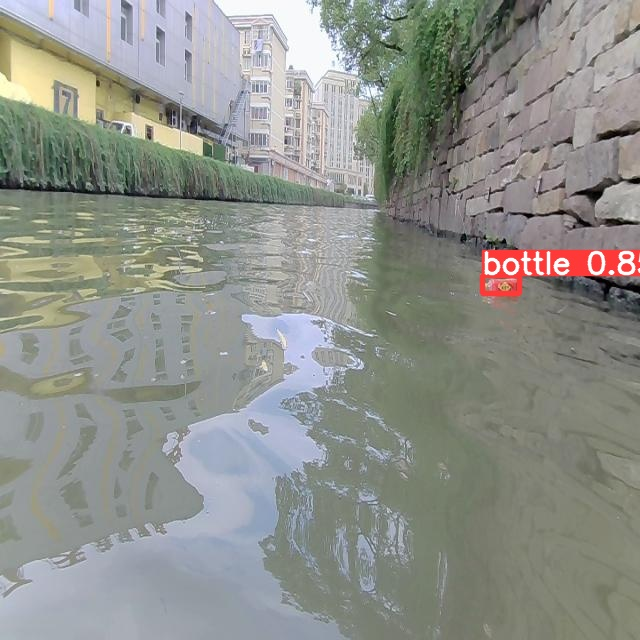
\includegraphics[width=0.45\textwidth]{images/test-img-1.png}}%
\hfill % <-- Seperation
\subcaptionbox{}
{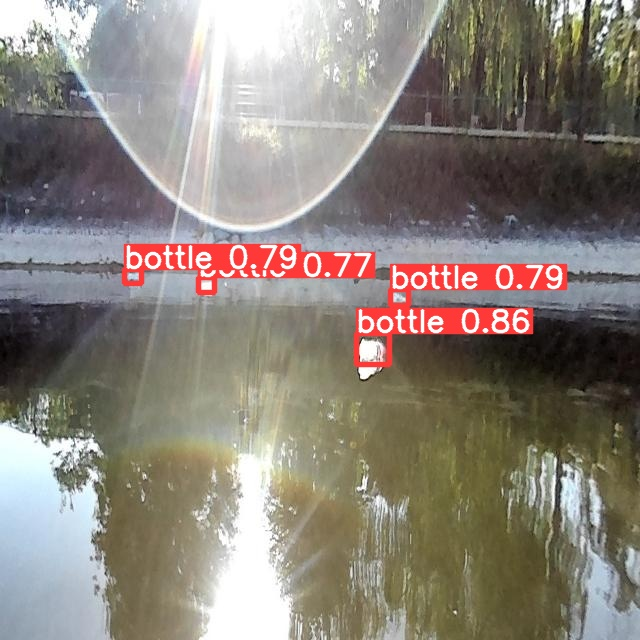
\includegraphics[width=0.45\textwidth]{images/test-image-2.png}}%
\caption{Test Images}
\label{fig:test}
\end{figure}

% \begin{figure}[H]
% \centering
% \subcaptionbox{Subcaption A}{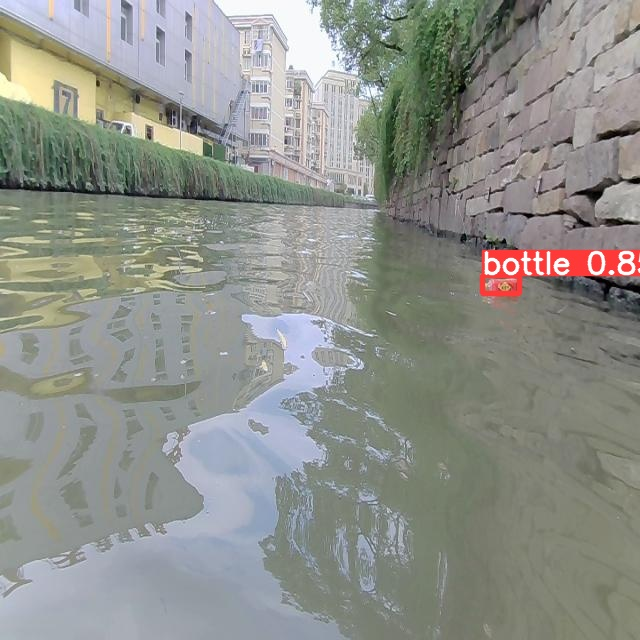
\includegraphics[width=0.30\textwidth]{images/test-img-1.png}}%
% \hfill
% \subcaptionbox{Subcaption B}{\includegraphics[width=0.30\textwidth]{images/test-img-2.png}}%
% \caption{Caption}
% \label{fig:nmbdmbkd}
% \end{figure}

%     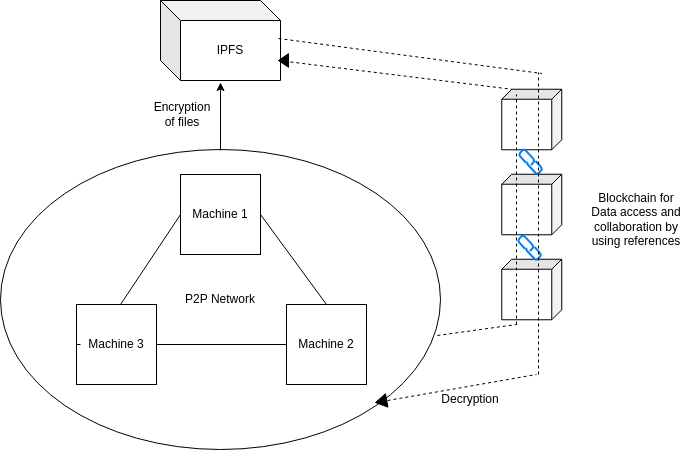
\includegraphics[width=14cm]{images/arch.png}
% \begin{center}
%     Proposed System Design
% \end{center}

% \newpage
% \section{Gantt Chart of Progress}
% \noindent\\\\
%     % \centering
%     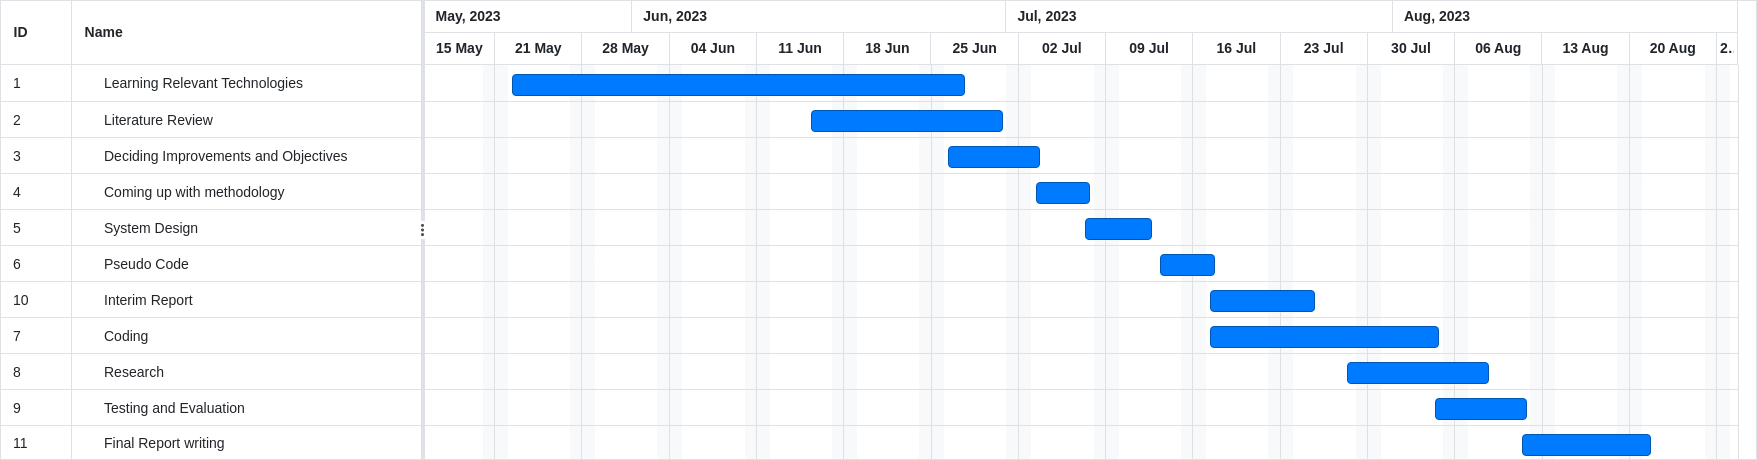
\includegraphics[width=16cm]{images/gantt.png}
% \subsection{Neural Network Architecture for Image Description Generation}
% \noindent The current study involves designing the architecture of the image description generation module using the encoder-decoder based method. Encoder will output the feature vector after taking image as the input. The feature vector will be given to the attention module and then a simple and efficient decoder will be selected to output the sequence of words as the image description. An overview of the proposed architecture is given in the figure \ref{fig:Chapter-4d}.

% \begin{figure}[h]
% \centering
% 	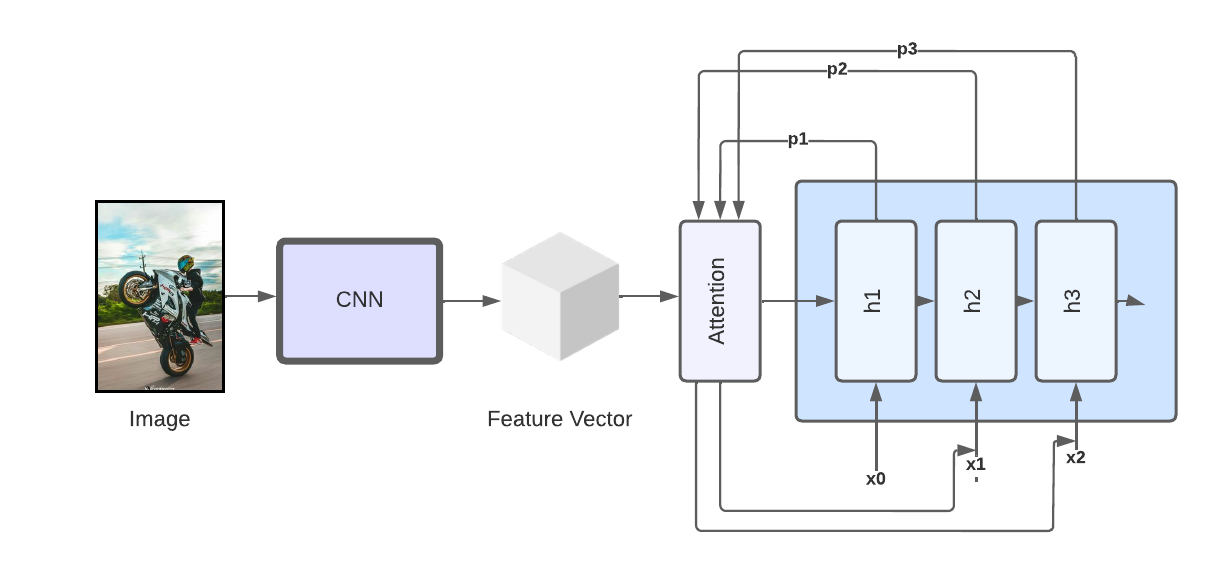
\includegraphics[scale=0.8]  {chapters/4/intfig/attention.png}
% 	  \caption{An overview of the proposed architecture of the image description generation module.}
% 	\label{fig:Chapter-4d}
% \end{figure}

% \noindent The encoder (CNN) in Figure \ref{fig:Chapter-4d} will return a feature vector of image which will be fed as input to the attention module. The attention module will compute attention weights for each iteration using the context and the feature vector. The attention weights will be multiplied with the feature vector and then will fed to sequence model (LSTM/GRU).

% \subsection{Automating Encoder Selection}
% \noindent There are various encoders that can be used to fetch the image vector representation. To deal with the uncertainty of the selection of encoder which gives the best result for image description generation. We will deploy all the models with various encoders and automate the selection of the encoder based on the matching labels obtained from object/label detection algorithm.
% \begin{figure}[h]
% \centering
% 	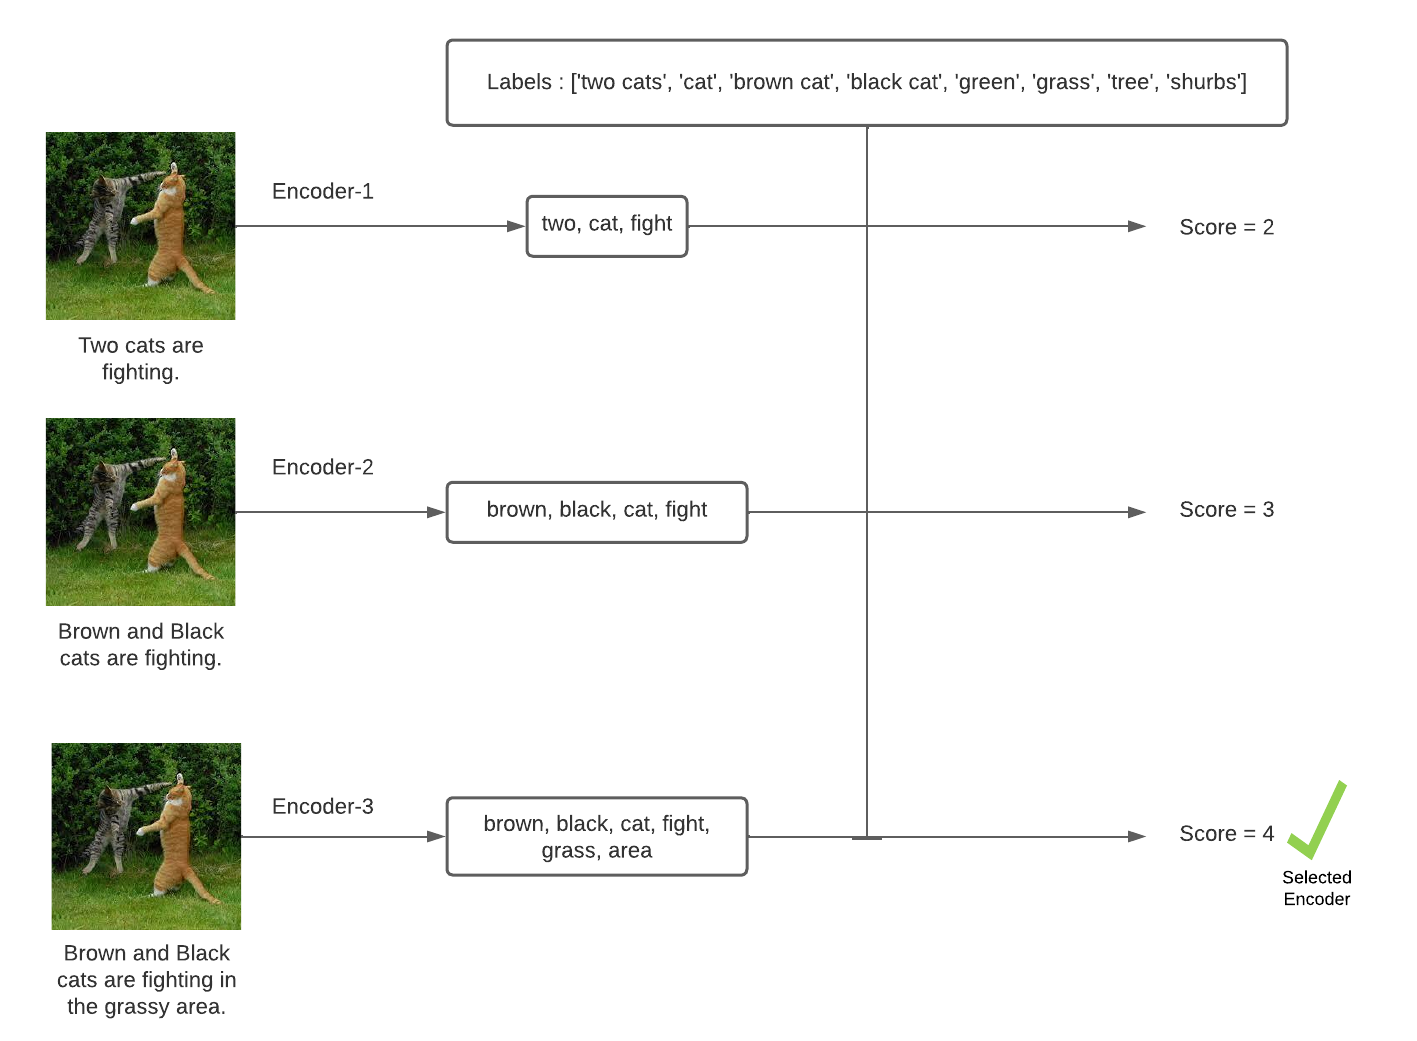
\includegraphics[scale=0.7]{chapters/4/intfig/automate.png}
% 	  \caption{Automating the selection of different encoders based on the labels obtained from the object detection algorithm.}
% 	\label{fig:Chapter-4d-automate}
% \end{figure}

% \noindent Figure \ref{fig:Chapter-4d-automate} describes, the method for automating the object detection. The labels will be generated by the object detection and caption will be generated by the various encoder-decoder model. Root word will be extracted from the captions and the score will be calculated based on number of root word matching with the labels. The model with the best score will be selected for sending the image description.

% \subsection{Design for Native Mobile Application}
% \noindent After, we have our efficient and simple model for generating image description. We will deploy our model on the cloud platform and will build an mobile application that will help the blind individual to click a photo and get the audio of the image description generated. 

% \begin{figure}[h]
% \centering
% 	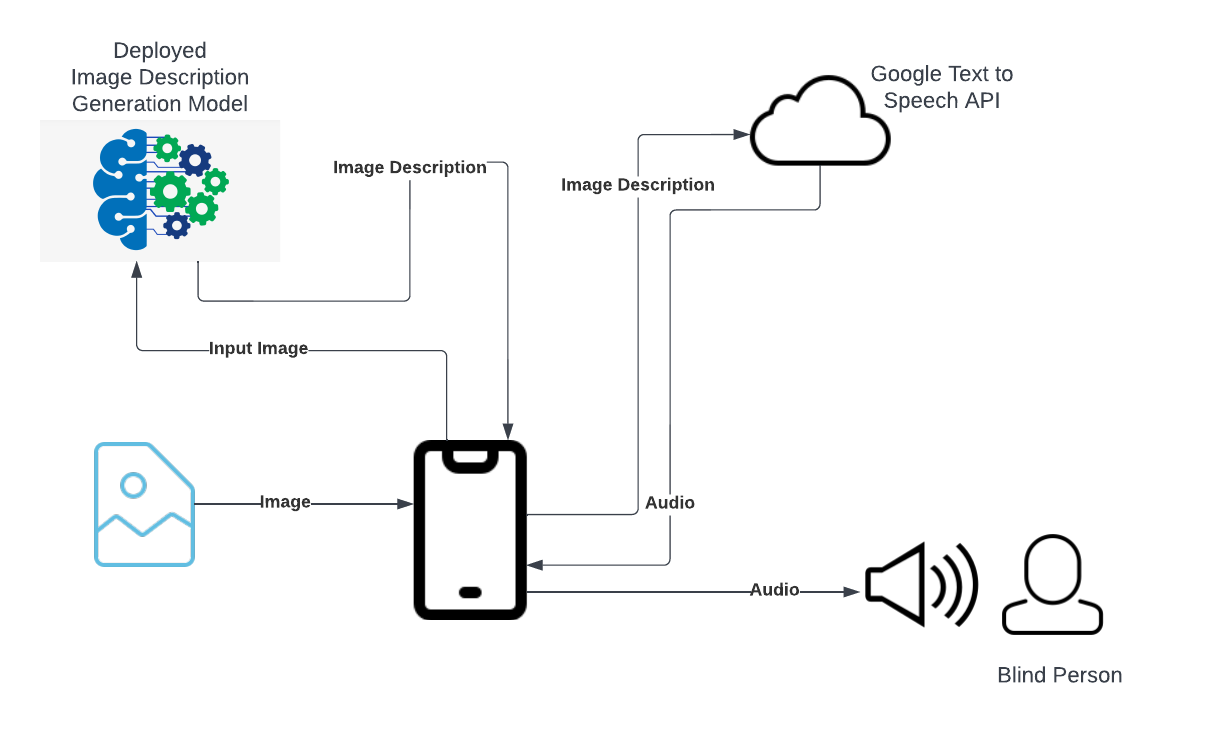
\includegraphics[scale=1.0]  {chapters/4/intfig/system_design.png}
% 	  \caption{An overview of the proposed architecture of the image description generation module.}
% 	\label{fig:Chapter-4d-system_design}
% \end{figure}

% \noindent The flow of the logic of the system described in the Figure \ref{fig:Chapter-4d-system_design} is as follows:
% \begin{enumerate}
%     \item The input will be taken from the native mobile application.
%     \item The user will request for the description of the image from the deployed ML model on the cloud.
%     \item The model will return the description sentence to the client side of the application.
%     \item Google's Text to Speech API will be used to convert the image's description to the audio.
%     \item The audio will be played for the blind person to tell them about the description of the image.
% \end{enumerate}
% % \noindent The first step required to establish a research in this area is to give input images, that are to be passed through a preprocessing phase. Preprocessing of images includes scaling, shifting, rotating etc. as per the  requirement on those particular images. Preprocessing also includes conversion of images such as from RGB to grayscale. Furthermore, at the processing stage itself filtering of noise is also established. After preprocessing comes the process of extraction of features from the image and the background. Extraction of features can be obtained from various means of skin segmentation, using various techniques. Followed by extraction of features comes modeling of features that is enhancing the discriminative powers of essential parameters for better processing and results. Then comes the phase of skin classification where the skin pixels are segregated into two parts that is skin pixels and non-skin pixels.
% % \begin{figure}[h]
% % \centering
% % 	\includegraphics*[height = 11cm, width = 13cm]{chapters/1/intfig/Block_diagram2.eps}
% % 	 \caption{Block diagram of our proposed methodology.}
% % 	\label{fig:Chapter-4a}
% % \end{figure}
% % \section{Work Done} 
% % We test the basics color models.That gives us the result.We obtain that the all these models insuficent to get the skin at same parameters. result will be shown in fig(i).
% % begin{figure}[h]
% % \centering
% % \includegraphics*[height = 11cm, width = 13cm]{chapters/1/intfig/Block_diagram2.eps}
% \newpage
% \section{Proposed methodology}
% \noindent The objective of the present study is to generate image description with good performance. The task of generating the image caption can be divided into two parts:
% \begin{enumerate}
%     \item Feature Extraction
%     \item Description Generation
% \end{enumerate}

% \subsection{Feature Extraction}
% \noindent Most of the studies conducted on image captioning have proved that encoder-decoder based architecture gives a rich description of the image with high performance. The three dimensional image is given as input to the encoder part of the architecture and image's feature representation is extracted as output of the encoder. Convolutional Neural Network (CNN) serves the purpose of the encoder. Generally, CNN performs manipulations on the image using the Convolution layer and Pooling Layer. It effectively reduces the dimensionality of the image without losing the necessary information or features captured in the image. Many pre-trained Convolutional Neural Network based architecture (ResNet, VGG, Inception) are present, which can reduce the time of training the image description generation model. \\
% The first task is to choose an efficient CNN model, considering the complexity and the performance of various CNN models. The parameters, accuracy and depth of the network of various CNN models is given in the Table \ref{table:1}. \\

% \begin{table}[h!]
%     \centering
%     \caption{CNN Models Accuracy, Parameters, Layers}
%     \begin{tabular}{ |c|c|c|c|c| } 
%      \hline
%      \textbf{S.No.} & \textbf{CNN Model} & \textbf{No. of Parameters} & \textbf{No. of Layers} & \textbf{Accuracy on ImageNet}\\ 
%      \hline
%      1 & VGG16 & 138,35,544 & 16 & 74.5\% \\ 
%      2 & Inception V3 & 23,851,784 & 42 & 78.8\% \\
%      3 & ResNet50 & 23,587,712 & 50 & 77.6\% \\
%      \hline
%     \end{tabular}
%     \label{table:1}
% \end{table}

% \newpage
% \subsubsection{VGG16}
% \noindent Visual Geometry Group (VGG) is a Convolutional Neural Network (CNN) architecture proposed by Karen {\em{et al.}} \cite{vgg}. VGG16 has 16 number of layers where weights are learned while training the model. VGG19 is also a Convolutional Neural Network model available which has 19 layers with weights. \\
% The VGG16 model takes a standard input image with size 244x244x3. It uses kernel filter of 3x3 size with stride 1. They use maxpool of size 2x2 with stride 2. The size of the kernel filter, maxpool filter and padding is constant throughout the model. The detailed architecture of VGG16 is given in the figure \ref{fig:vgg16_architecture}. 

% \usetikzlibrary{positioning,fit,calc}
% \tikzset{block/.style={draw, thick, text width=6cm, minimum height=0.5cm, align=center},   
% line/.style={-latex}
% }  

% \begin{figure}
%     \centering
%     \begin{tikzpicture}   
%       \node[block] (o) {\small Output};  
%       \node[block] (n) at ([yshift=-0.9cm]$(o)$) {\footnotesize Softmax};  
%       \node[block] (m) at ([yshift=-0.9cm]$(n)$) {\footnotesize Fully Connected};  
%       \node[block] (l) at ([yshift=-0.9cm]$(m)$) {\footnotesize Fully Connected};  
%       \node[block] (k) at ([yshift=-0.9cm]$(l)$) {\footnotesize Max Pooling};  
%       \node[block] (j) at ([yshift=-0.9cm]$(k)$) {\footnotesize 3 x Convolution 512};  
%       \node[block] (i) at ([yshift=-0.9cm]$(j)$) {\footnotesize Max Pooling};  
%       \node[block] (h) at ([yshift=-0.9cm]$(i)$) {\footnotesize 3 x Convolution 512};  
%       \node[block] (g) at ([yshift=-0.9cm]$(h)$) {\footnotesize Max Pooling};  
%       \node[block] (f) at ([yshift=-0.9cm]$(g)$) {\footnotesize 3 x Convolution 256};  
%       \node[block] (e) at ([yshift=-0.9cm]$(f)$) {\footnotesize Max Pooling};  
%       \node[block] (d) at ([yshift=-0.9cm]$(e)$) {\footnotesize 2 x Convolution 128};  
%       \node[block] (c) at ([yshift=-0.9cm]$(d)$) {\footnotesize Max Pooling};  
%       \node[block] (b) at ([yshift=-0.9cm]$(c)$) {\footnotesize 2 x Convolution 64};  
%       \node[block] (a) at ([yshift=-0.9cm]$(b)$) {\footnotesize Input Image};   

%       \node[right=of a] {\footnotesize 244 x 244 x 3};
%       \node[right=of b] {\footnotesize 244 x 244 x 64};
%       \node[right=of c] {\footnotesize 112 x 112 x 64};
%       \node[right=of d] {\footnotesize 112 x 112 x 128};
%       \node[right=of e] {\footnotesize 56 x 56 x 128};
%       \node[right=of f] {\footnotesize 56 x 56 x 256};
%       \node[right=of g] {\footnotesize 28 x 28 x 256};
%       \node[right=of h] {\footnotesize 28 x 28 x 512};
%       \node[right=of i] {\footnotesize 14 x 14 x 512};
%       \node[right=of j] {\footnotesize 14 x 14 x 512};
%       \node[right=of k] {\footnotesize 7 x 7 x 512};
%       \node[right=of l] {\footnotesize 4096};
%       \node[right=of m] {\footnotesize 4096};
%       \node[right=of n] {\footnotesize 1000};

      
%       \draw[line] (a)-- (b);
%       \draw[line] (b)-- (c);
%       \draw[line] (c)-- (d);
%       \draw[line] (d)-- (e);
%       \draw[line] (e)-- (f);
%       \draw[line] (f)-- (g);
%       \draw[line] (g)-- (h);
%       \draw[line] (h)-- (i);
%       \draw[line] (i)-- (j);
%       \draw[line] (j)-- (k);
%       \draw[line] (k)-- (l);
%       \draw[line] (l)-- (m);
%       \draw[line] (m)-- (n);
%       \draw[line] (n)-- (o);
%     \end{tikzpicture}  
%     \caption{The architecture of the pre-trained CNN model, VGG16 \cite{vgg}}
%     \label{fig:vgg16_architecture}
% \end{figure}

% \subsubsection{Inception}
% \noindent Inception V3 is also a CNN pre-trained model published in 2015 \cite{inception}. It performed better than its subsequent parts like V1 and V2. There were many major advancements that led to increase in the performance of Inception V3. It factorized the convolutions into many smaller convolutions, a convolution was spillted to many asymmetric convolution to reduce the computation. In total, the Inception V3 consisted of 42 layers. A constrained view of the Inception model is given in the figure \ref{fig:inceptionv3_architecture}.
% \begin{figure}[h!]
%     \centering
%     \begin{tikzpicture}   
%       \node[block] (o) {\small Output};  
%       \node[block] (n) at ([yshift=-0.9cm]$(o)$) {\footnotesize Softmax};  
%       \node[block] (m) at ([yshift=-0.9cm]$(n)$) {\footnotesize Fully Connected};  
%       \node[block] (l) at ([yshift=-0.9cm]$(m)$) {\footnotesize Global Avg. Pooling};  
%       \node[block] (k) at ([yshift=-0.9cm]$(l)$) {\footnotesize 2 x Inception C};  
%       \node[block] (j) at ([yshift=-0.9cm]$(k)$) {\footnotesize Reduction B};  
%       \node[block] (i) at ([yshift=-0.9cm]$(j)$) {\footnotesize 4 x Inception B};  
%       \node[block] (h) at ([yshift=-0.9cm]$(i)$) {\footnotesize Reduction A};  
%       \node[block] (g) at ([yshift=-0.9cm]$(h)$) {\footnotesize 3 x Inception A};  
%       \node[block] (f) at ([yshift=-0.9cm]$(g)$) {\footnotesize Max Pooling 3*3/2};  
%       \node[block] (e) at ([yshift=-0.9cm]$(f)$) {\footnotesize Convolution 3*3 (192/1)};  
%       \node[block] (d) at ([yshift=-0.9cm]$(e)$) {\footnotesize Convolution 1*1 (80/1)};  
%       \node[block] (c) at ([yshift=-0.9cm]$(d)$) {\footnotesize Max Pooling 3*3/2};  
%       \node[block] (b) at ([yshift=-0.9cm]$(c)$) {\footnotesize 3 x Convolution 3*3};  
%       \node[block] (a) at ([yshift=-0.9cm]$(b)$) {\footnotesize Input Image};   

%       \node[right=of a] {\footnotesize 299 x 299 x 3};
%       \node[right=of b] {\footnotesize 147 x 147 x 64};
%       \node[right=of c] {\footnotesize 73 x 73 x 64};
%       \node[right=of d] {\footnotesize 73*73*80};
%       \node[right=of m] {\footnotesize 2048};
%       \node[right=of n] {\footnotesize 1000};

      
%       \draw[line] (a)-- (b);
%       \draw[line] (b)-- (c);
%       \draw[line] (c)-- (d);
%       \draw[line] (d)-- (e);
%       \draw[line] (e)-- (f);
%       \draw[line] (f)-- (g);
%       \draw[line] (g)-- (h);
%       \draw[line] (h)-- (i);
%       \draw[line] (i)-- (j);
%       \draw[line] (j)-- (k);
%       \draw[line] (k)-- (l);
%       \draw[line] (l)-- (m);
%       \draw[line] (m)-- (n);
%       \draw[line] (n)-- (o);
%     \end{tikzpicture}  
%     \caption{The architecture of the pre-trained CNN model, Inception V3 \cite{inception}}
%     \label{fig:inceptionv3_architecture}
% \end{figure}

% \subsubsection{ResNet50}
% \noindent The ResNet architecture was proposed to solve the problem of the vanishing gradient commonly seen in the CNN models. The problem was resolved using the skip connections between the different layers \cite{resenet}. ResNet50 architecture was 50 layers deep and had fewer parameters than the VGG16 and Inception V3 architecture. Though, the model will be difficult to train because of the increase in the depth but will certainly have better performance. The architecture of ResNet50 is given in the figure \ref{fig:resnet}.
% \begin{figure}[h!]
% \centering
% 	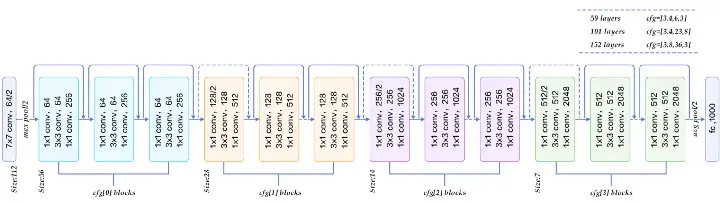
\includegraphics[scale=0.7]  {chapters/4/intfig/resnet.png}
% 	  \caption{The architecture of the pre-trained CNN model, ResNet50 \cite{resenet}}
% 	\label{fig:resnet}
% \end{figure}
% \subsubsection{Feature Vector Representation of Image}
% \noindent Consider, image $I$ is fed into any selected convolutional neural network model. The output of the encoder will be the visual representation of the features of the image. Let's say $F$ is the feature vector received as output after fully connected layer of CNN and $V$ is the spatial vector received as output from the last convolution layer of CNN.
% \begin{equation}
%     F = C_{fc}(I)
% \end{equation}
% \begin{equation}
%     V = C_{conv}(I)
% \end{equation}

% \noindent Here, $C_{fc}$ is the output of the fully connected later of CNN and $C_{conv}$ is the output of the last convolution later of CNN.
% \begin{equation}
%     V=\{v_{1}, v_{2}, ...., v_{k^2}\}
% \end{equation}
% The output of the last convolution layer $V$ is the visual $k$ x $k$ grid which can map to the previous convolution layer outputs and can perfectly define the relative feature positions. \\
% The fully connected layer output $F$ will be given as input to the decoder or language model in model where no attention mechanism is adopted, while the $F$ will be the input to the attention module in the attention mechanism model of image description generation.

% \subsection{Description Generation}
% \noindent The task of image description generation deals with the generation of sequence of words. The idea of generation of sequence of words make us use the Recurrent Neural Network (RNN). \\
% Consider $I$ is the input image and $\theta$ is the model parameter to be trained. The aim of the model is to generate sentence $S$ by maximising the likelihood of the expression.
% \begin{equation}
%     \theta^{*} = \arg \max_{\theta} \sum (I,S) \log p(S|I;\theta)
% \end{equation}
% \begin{equation}
%     h_{t+1} = f(h_{t},x_{t})
% \end{equation}
% The generation of the next hidden state $(h_{t+1})$ is a non-linear function $(f)$ of the previous hidden state and the context word $(h_{t})$. The naive RNN network fails to deal with the long sequence of words because of the exploding gradients words get vanished with time. Many researches conducted on image caption generation adopted LSTM as the language generation model as it solves the problem discussed aforementioned. \\
% In our study we will be experimenting with both LSTM and GRU model. GRU is simpler RNN model with not only solves the above mentioned problem but also requires lesser parameter to train. It is an effort to reduce the complexity of the decoder section of the architecture. 
% \subsubsection{LSTM - Long Short-Term Memory}
% \begin{figure}[h]
% \centering
% 	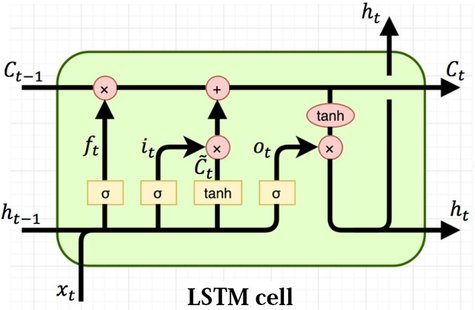
\includegraphics  {chapters/4/intfig/lstm.png}
% 	  \caption{The basic architecture of the repeating module of LSTM \cite{lstm}}
% 	\label{fig:Chapter-4a}
% \end{figure}
% \noindent LSTM is a variation of the recurrent neural network. It consist of three gates: input gate, output gate and the forget gate. The value of previous hidden state, $h_{t-1}$ and the current element of the sentence $x_{t}$ is passed through the sigmoid function.
% \begin{equation}
%     f_{t} = \sigma(W_{f}.[h_{t-1},x_{t}]+b_{f})
% \end{equation}
% Now, we need to decide through the input layer, $i_{t}$ which values needs to be updated and set of all the possible candidates that could be the next potential $C_{t}$.
% \begin{equation}
%     i_{t} = \sigma(W_{i}.[h_{t-1},x_{t}]+b_{i})
% \end{equation}
% \begin{equation}
%     \Tilde{C_{t}} = \tanh(W_{C}.[h_{t-1},x_{t}]+b_{c})
% \end{equation}
% $C_{t-1}$ will be updated to $C_{t}$ using the formula given below.
% $$C_{t} = f_{t}*C_{t-1} + i_{t}*\Tilde{C_{t}}$$
% The output of the hidden state of this iteration will be decided using the sigmoid and the hyperbolic function.
% \begin{equation}
%     o_{t} = \sigma(W_{o} [h_{t-1},x_{t}] + b_{o})
% \end{equation}
% \begin{equation}
%     h_{t} = o_{t}*\tanh(C_{t})
% \end{equation}

% \noindent The $C{t}$ and $h_{t}$ will be fed as input to the LSTM at $t+1$ iteration. At every iteration, the $h_{t}$ given to the softmax function to get the distribution of probability of every word from the dataset. 
% \subsubsection{GRU - Gated Recurrent Unit}
% \begin{figure}[h]
% \centering
% 	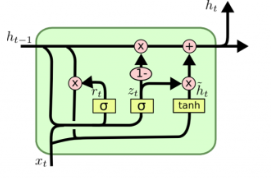
\includegraphics  {chapters/4/intfig/gru.png}
% 	  \caption{The basic architecture of the repeating module of GRU \cite{gru}}
% 	\label{fig:Chapter-4a}
% \end{figure}
% \noindent GRU is also a version of recurrent neural network solving the problem of long-term dependency very efficient. The model is not very complex and requires lesser parameters to be trained than the LSTM model. The GRU architecture only gives the hidden state $h_{t}$ and no $C_{t}$ as the output. This architecture is faster to train. This network contains: update gate $(z_{t})$ and reset gate $(r_{t})$. These gates decide the value of the hidden state $(h_{t})$ that will given as input to the GRU for next iteration.
% \begin{equation}
%     z_{t} = \sigma(W_{z}x_{t} + U_{z}h_{t-1}+b_{z})
% \end{equation}
% \begin{equation}
%     r_{t} = \sigma(W_{r}x_{t} + U_{r}h_{t-1}+b_{r})
% \end{equation}
% \begin{equation}
%     h_{t} = (1-z_{t}) \cdot h_{t-1} + z_{t} \cdot \tanh(W_{h}x_{t} + U_{h}(r_{t}\cdot h_{t-1}) + b_{h})
% \end{equation}

% \noindent At every iteration, the $h_{t}$ given to the softmax function to get the distribution of probability of every word from the dataset. 
% \subsection{Visual Attention}
% \begin{figure}[h]
% \centering
% 	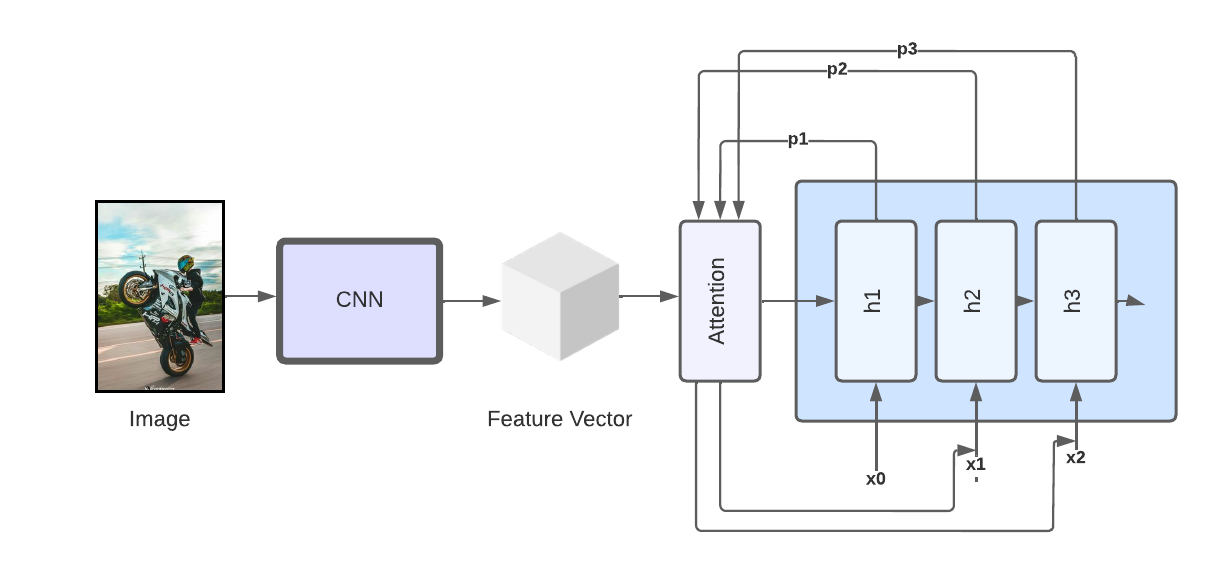
\includegraphics[scale=0.8]  {chapters/4/intfig/attention.png}
% 	  \caption{Encoder-Decoder based architecture for image description generation using attention module}
% 	\label{fig:Chapter-4a}
% \end{figure}
% \noindent The idea of the attention mechanism comes from the attention used for the image classification, as all of the pixels are of no use to classify the image. In attention-based image description generation, the output of the convolutional fully connected layer fed into the attention module. With attention gate, the decoder concentrate on only those pixel of the image that are relevant. In each iteration, the feature vector representation of the image and previous context of the LSTM or GRU is given to the attention module. The attention module then calculates the weight of the attention vector. The attention mechanism is differentiable. The training of the attention mechanism can be done using the backpropagation.
% \begin{equation}
%     a_{t} = \sum_{1}^{n} S_{j}Y_{j}
% \end{equation}
% Here, $a_{t}$ is the attention vector obtained after training. $S$ is the function that gives the output after performing the softmax operation. $Y$ is the feature representation of the image.


% \section{Evaluation metrics}
% \noindent The description of the images generated needs to be rich in the information displayed, readable and grammatically correct. This is a supervised learning module where we have the predicted description along with the reference description. The evaluation metrics measures how much the predicted description matches with the true description. In our study, we will be checking the performance of our model on evaluation metric like BLEU, GLEU, METEOR. \\
% BLEU score is evaluated by first calculating the n-gram of the predicted description and the true description \cite{bleu}. Then it counts the matching in the respective n-grams. This score was majorly defined to evaluate the performance of the translation of the languages model. The structure of the description is not taken into consideration in the BLEU score. A model should achieve atleast a BLEU score of more than 0.5 for valid consideration. \\
% METEOR score worked on the disadvantage of the BLEU score. This evaluation metric uses the WordNet for matching the resemblance between the predicted description and true description. It also calculates the resemblance between the synonyms, suffix, prefix and the roots of the sentences, making it closer to the human discrimination \cite{meteor}.
% \begin{equation}
%    METEOR = 10* Precision * \frac{Recall}{Recall + 9 * Precision} 
% \end{equation}
% METEOR uses the Precision and Recall to calculate the score. Recall is given more weightage than the Precision making it more closer to the human description. \\
% GLEU is another evaluation metric to check the performance of the image description module with respect to the grammatical errors and the fluency of the generated sentences. The n-gram of the generated description is overlapped with the different sentences. GLEU score is identical to the BLEU score with respect to the computation.


% \section{Dataset}
% \noindent \textbf{Flickr8k} dataset will be used to evaluate the performance of the image description generation and also for training the model. The dataset consist of 8000 images which can be splitted in the ratio of 6:1:1 for training, validation and testing purpose respectively. In the dataset, for each and every image there are five descriptions. There is also Flickr30k dataset which consist of 30,000 images in total. The performance of the model will increase with the number of the images used for training the model. So, Flickr30k dataset will be used to improve the performance of the model \cite{flickr30k}.\\
% \noindent \textbf{MSCOCO} dataset is also similar with respect to the structure, it also contains five descriptions for each image. Total number of images in the dataset is around 164K. The training set can have 84K images, validation set and testing set can contain 40K images each \cite{mscoco}. Due, to hardware constraint we will restrict our training with Flickr dataset. 

% \section{Text-To-Speech (TTS) Conversion}
% \noindent In our study, the description obtained from the neural network model will be converted to the waveforms, audio for assisting the blind person about the image. We will be using Google's Text-To-Speech API for performing the mentioned task. \\
% The API works on the Tacotron 2 \cite{tacotron2}, proposed by the engineers of Google. It is a neural network architecture for generating the audio version of the text (speech synthesis). The neural network architecture works on Seq2Seq model, where inputs are the sequence of word embeddings and output is mel-scale spectrograms, which is sequence of waveforms for audio. The architecture comprises of two major components, (i) RNN Seq2Seq Model with attention module which takes input as the sequence of words and produces mel spectrogram sequence, and (ii) WaveNet \cite{wavenet} which takes predicted mel spectrogram frames as input and convert it to waveforms for raw audio which is much more closer to the human speech. This model achieved mean opinion score(MOS) of 4.53 much closer to professional human speech.\label{chap:problem_statement}


% \chapter{Conclusion and Future Scope}
% \vspace{-1cm}
% \noindent \rule{6.6in}{0.01in}
% \clearpage
\noindent This chapter details the project's conclusion and the thesis's future scope.

\section{Conclusions}
\noindent In this study, we examined the vital challenge of surface floating object detection using the FloW dataset and novel object detection models, particularly GroundedSAM and YOLOv8. In order to automatically annotate images and produce a dataset for training the target model, we made use of the capability of knowledge distillation. We achieved precise and quick floating waste detection by combining the capabilities of GroundedSAM's automatic annotating and YOLOv8's effective real-time detection.
Results showed that our method identified and classified floating waste objects in challenging conditions, including those involving reflections and too much light. The distilled model, developed by transferring knowledge from GroundedSAM to YOLOv8, demonstrated impressive performance, showcasing its potential as a potent tool for practical applications like pollution monitoring, environmental conservation, and search and rescue.

\section{Future Scope}
\noindent A complete analysis of previous methods and approaches used for image description generation has been done in the literature review process.
\begin{enumerate}
    \item Training the final model on the more diverse dataset and leveraging the power of prompt engineering to improve the performance of the model.
    \item Try out various hyperparameter configurations for GroundedSAM and YOLOv8. Various factors, including learning rates, batch sizes, optimizer selections, and regularisation methods.
    \item Find the ideal parameters for efficiently transferring knowledge from GroundedSAM to YOLOv8, extending hyperparameter adjustment to the knowledge distillation procedure.
    \textbf{dont add as bullets, rewrite as whole paragraph and write this in detail}
\end{enumerate}\label{chap:cons_fscope}

% ---------------------------- End - ------


%\clearpage
%\mbox{}
%\thispagestyle{empty}
%\newpage


% \chapter{Results and Discussions}
% \vspace{-1cm}
% \noindent \rule{6.6in}{0.01in}
% \clearpage
\noindent This chapter details about the work done till now and the results obtained.
\section{Activities Completed}
\begin{enumerate}
    \item Filtered recent research papers on image description generation using various architecture. From the literature review, found out the literature gaps in recent researches and generated the problem statement.
    \item Completed the image description generation task using Flicker8k dataset with various pre-trained encoders: VGG16, Inception V3 and ResNet50 combined with RNN decoders: LSTM and GRU with and without attention.
    \item Calculated the BLEU-1, BLEU-2, METEOR, GLEU score for all the above mentioned encoder-decoder architecture.
    \item Selected GRU as the decoder based on the time required to train the model.
    \item Deployed all the models and automated the process of selecting the encoders based on the labels obtained from the object detection algorithm.
    \item Built the native mobile application that takes the input as image and predict the description. Converted the generated text description to audio using the Google Text-To-Speech
API.
\end{enumerate}

\section{Results}
\subsection{Encoder-Decoder Image Description Model}
\noindent In our study we adopted encoder-decoder based architecture for generating the image description. We performed an experimental analysis by combining various pre-trained CNN models (encoders) : VGG16, Inception V3, ResNet50, with various sequence generating models (decoders): LSTM and GRU with and without attention mechanism. \\ \\
\noindent The Table \ref{table:2} gives detail of the BLEU-1, BLEU-2 score and Table \ref{table:3} gives detail of the METEOR and GLEU score of above mentioned architectures without attention while training on the Flickr8k dataset. The Table \ref{table:4} gives detail about the time required for training with various model for 20 epochs and 32 batches without attention. \\

\begin{table}[h!]
    \centering
    \caption{BLEU Score for image description model with various encoder and decoder without attention on Flickr8k dataset.}
    \begin{tabular}{ |c|c|c|c|c|c| } 
     \hline
     \textbf{S.No.} & \textbf{Encoder} & \textbf{Decoder} & \textbf{Attention} & \textbf{BLEU-1 Score} & \textbf{BLEU-2 Score}\\ 
     \hline
     1 & VGG16 & LSTM & No & 0.536422 & 0.307395 \\ 
     \hline
     2 & Inception V3 & LSTM & No & \textbf{0.565980}	&  \textbf{0.337752} \\
     \hline
     3 & ResNet50 & LSTM & No & 0.558754 & 0.334540 \\
     \hline
     4 & VGG16 & GRU & No & 0.542930 & 0.313084 \\
     \hline
     5 & Inception V3 & GRU & No & 0.555470 & 0.332273 \\
     \hline
     6 & ResNet50 & GRU & No & 0.551240 & 0.321962 \\
     \hline
    \end{tabular}
    \label{table:2}
\end{table}

\noindent In the Table \ref{table:2}, Inception V3 + LSTM neural network architecture gives the best BLEU-1 and BLEU-2 score, but Inception V3 + GRU neural network architecture gives comparable result. \\

\begin{table}[h!]
    \centering
    \caption{METEOR and GLEU Score for image description model with various encoder and decoder without attention on Flickr8k dataset.}
    \begin{tabular}{ |c|c|c|c|c|c| } 
     \hline
     \textbf{S.No.} & \textbf{Encoder} & \textbf{Decoder} & \textbf{Attention} & \textbf{METEOR Score} & \textbf{GLEU Score}\\ 
     \hline
     1 & VGG16 & LSTM & No & 0.385067 & 0.160952	 \\ 
     \hline
     2 & Inception V3 & LSTM & No & \textbf{0.400490} & \textbf{0.173167} \\
     \hline
     3 & ResNet50 & LSTM & No & 0.398279 & 0.171752 \\
     \hline
     4 & VGG16 & GRU & No & 0.374429 & 0.162264	 \\
     \hline
     5 & Inception V3 & GRU & No & 0.395749 & 0.169225	\\
     \hline
     6 & ResNet50 & GRU & No & 0.386446 & 0.165116 \\
     \hline
    \end{tabular}
    \label{table:3}
\end{table}
\noindent In the Table \ref{table:3},  Inception V3 + LSTM neural network architecture gives the best METEOR and GLEU score, but Inception V3 + GRU neural network architecture gives comparable result.

\begin{table}[h!]
    \centering
    \caption{Training time in min(s) for image description model with various encoder and decoder without attention on Flickr8k dataset.}
    \begin{tabular}{ |c|c|c|c| } 
     \hline
     \textbf{S.No.} & \textbf{Encoder} & \textbf{Decoder} & \textbf{Training Time (min(s))}\\ 
     \hline
     1 & VGG16 & LSTM & 94	 \\ 
     \hline
     2 & Inception V3 & LSTM & 92 \\
     \hline
     3 & ResNet50 & LSTM & 92 \\
     \hline
     4 & VGG16 & GRU & 86	 \\
     \hline
     5 & Inception V3 & GRU & \textbf{84}	\\
     \hline
     6 & ResNet50 & GRU & 91 \\
     \hline
    \end{tabular}
    \label{table:4}
\end{table}
\newpage
\noindent In the Table \ref{table:4}, Inception V3 + GRU neural network architecture gives the least training time because GRU more is less complex than LSTM. In, Table \ref{table:2} & Table \ref{table:3} GRU decoder gave comparable results to LSTM and training time is also less. Hence, we would be considering GRU as our decoder for further study. 

\begin{figure*}[ht!]
    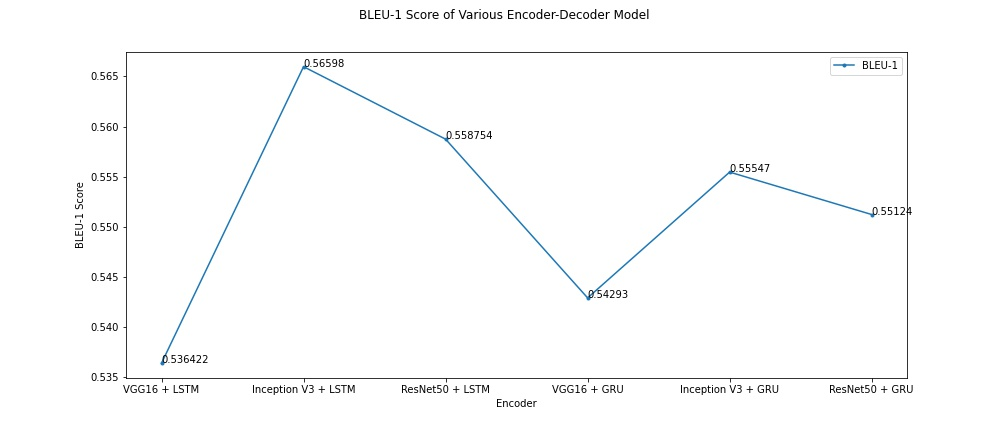
\includegraphics[scale=0.5]{chapters/5/intfig/bleu_score.jpg}\hfill
    \caption{Graphical comparision of BLEU score of different encoder-decoder models without attention on Flickr8k dataset.}
    \label{img:graph_bleu}
\end{figure*}
\noindent In the Figure \ref{img:graph_bleu}, Inception V3 + LSTM neural network architecture gives the best BLEU score, but Inception V3 + GRU neural network architecture gives comparable result.

\begin{figure*}[ht!]
    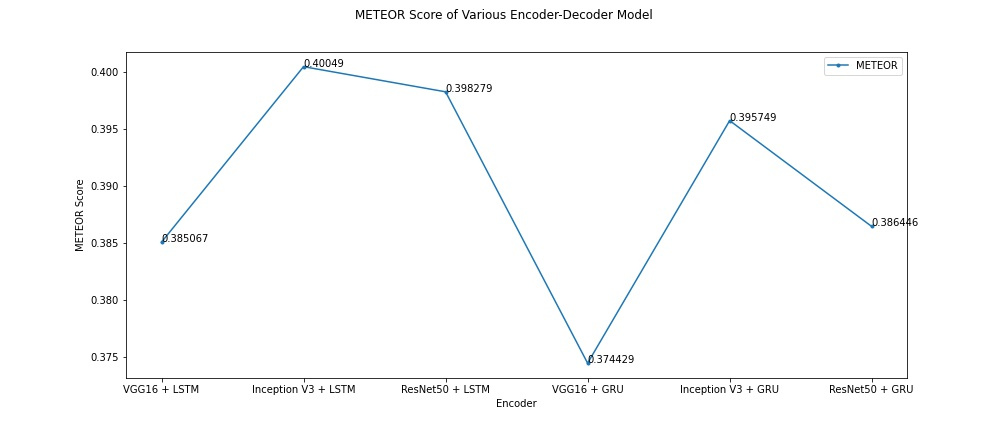
\includegraphics[scale=0.5]{chapters/5/intfig/meteor_score.jpg}\hfill
    \caption{Graphical comparision of METEOR score of different encoder-decoder models without attention on Flickr8k dataset.}
    \label{img:graph_meteor}
\end{figure*}
\newpage
\noindent In the Figure \ref{img:graph_meteor}, Inception V3 + LSTM neural network architecture gives the best METEOR score, but Inception V3 + GRU neural network architecture gives comparable result.

\begin{figure*}[ht!]
    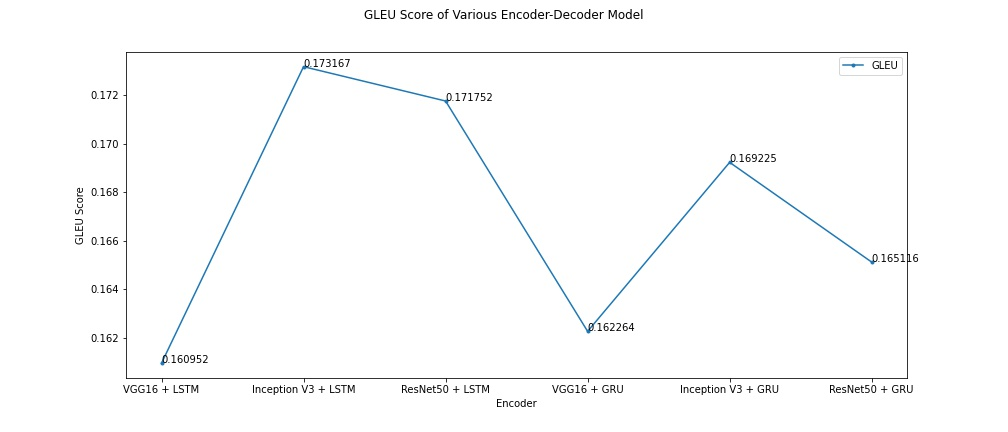
\includegraphics[scale=0.5]{chapters/5/intfig/gleu_score.jpg}\hfill
    \caption{Graphical comparision of GLEU score of different encoder-decoder models without attention on Flickr8k dataset.}
    \label{img:graph_gleu}
\end{figure*}
\noindent In the Figure \ref{img:graph_gleu}, Inception V3 + LSTM neural network architecture gives the best GLEU score, but Inception V3 + GRU neural network architecture gives comparable result.

\begin{figure*}[ht!]
    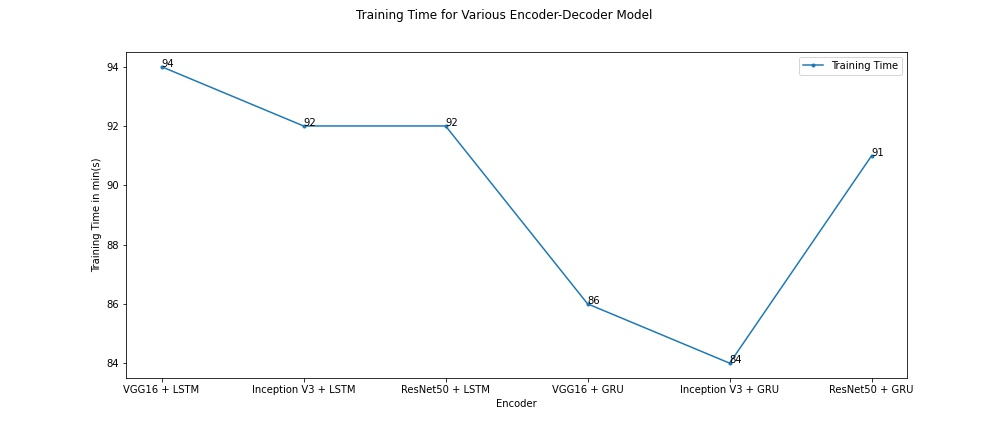
\includegraphics[scale=0.5]{chapters/5/intfig/training_time.jpg}\hfill
    \caption{Graphical comparision for training time of different encoder-decoder models without attention on Flickr8k dataset.}
    \label{img:graph_tt}
\end{figure*}
\noindent Figure \ref{img:graph_tt} shows, Inception V3 + GRU neural network architecture gives the least training time because GRU more is less complex than LSTM. \\ \\ 
\noindent The above graph Figure \ref{img:graph_bleu}, Figure \ref{img:graph_meteor} and Figure \ref{img:graph_gleu}, demonstrates that Inception V3 + LSTM performs best when tested for Flicker8k dataset on various evaluation metrics like BLEU, METEOR and GLEU score. But, Inception V3 + GRU model takes lesser time to train on the same hardware resources and dataset. The BLEU, METEOR and GLEU score also is comparable with the results of the best model. So, we will be considering \textbf{GRU} as our decoder model for further study of image description generation. \\ \\
\noindent The Table \ref{table:5} gives detail of the BLEU-1, BLEU-2 score and Table \ref{table:6} gives detail of the METEOR and GLEU score of various encoders with GRU decoder with attention while training on the Flickr8k dataset. The Table \ref{table:7} gives detail about the time required for training with various model for 20 epochs and 32 batches with attention.

\begin{table}[h!]
    \centering
    \caption{BLEU Score for image description model with various encoder and decoder with attention on Flickr8k dataset.}
    \begin{tabular}{ |c|c|c|c|c|c| } 
     \hline
     \textbf{S.No.} & \textbf{Encoder} & \textbf{Decoder} & \textbf{Attention} & \textbf{BLEU-1 Score} & \textbf{BLEU-2 Score}\\ 
     \hline
     1 & VGG16 & GRU & Yes & 0.544142 & 0.332934 \\
     \hline
     2 & Inception V3 & GRU & Yes & 0.586869 & \textbf{0.338021} \\
     \hline
     3 & ResNet50 & GRU & Yes & \textbf{0.596845} & 0.337755 \\
     \hline
    \end{tabular}
    \label{table:5}
\end{table}
\newpage
\noindent In the Table \ref{table:5}, Resnet50 gives the best BLEU-1 score, while Inception V3 gives the best BLEU-2 score. The table demonstrates the uncertainty between the encoders.

\begin{table}[h!]
    \centering
    \caption{METEOR and GLEU Score for image description model with various encoder and decoder with attention on Flickr8k dataset.}
    \begin{tabular}{ |c|c|c|c|c|c| } 
     \hline
     \textbf{S.No.} & \textbf{Encoder} & \textbf{Decoder} & \textbf{Attention} & \textbf{METEOR Score} & \textbf{GLEU Score}\\ 
     \hline
     4 & VGG16 & GRU & Yes & 0.454923 & 0.174830	 \\
     \hline
     5 & Inception V3 & GRU & Yes & 0.436624 & 0.172741	\\
     \hline
     6 & ResNet50 & GRU & Yes & \textbf{0.515464} & \textbf{0.206574} \\
     \hline
    \end{tabular}
    
    \label{table:6}
\end{table}
\noindent Table \ref{table:6} shows that Resnet50 gives the best METEOR and GLEU score amongst all the other encoders.

\begin{table}[h!]
    \centering
    \caption{Training time in min(s) for image description model with various encoder and decoder with attention on Flickr8k dataset.}
    \begin{tabular}{ |c|c|c|c| } 
     \hline
     \textbf{S.No.} & \textbf{Encoder} & \textbf{Decoder} & \textbf{Training Time (min(s))}\\ 
     \hline
     4 & VGG16 & GRU & \textbf{240}	 \\
     \hline
     5 & Inception V3 & GRU & 275	\\
     \hline
     6 & ResNet50 & GRU & 280 \\
     \hline
    \end{tabular}
    \label{table:7}
\end{table}

 \noindent GRU gave the best training time as showed in Table \ref{table:4}. But, amongst the various encoder VGG16 in the Table \ref{table:7} took the least time to train the model, because of the less number of layers to train in VGG16 encoder model. But, we cannot compromise with the accuracy of the image description generation. Hence, to resolve the uncertainity between different encoders, we will automate the selection of encoders.
 
\newpage
\begin{figure*}[ht!]
    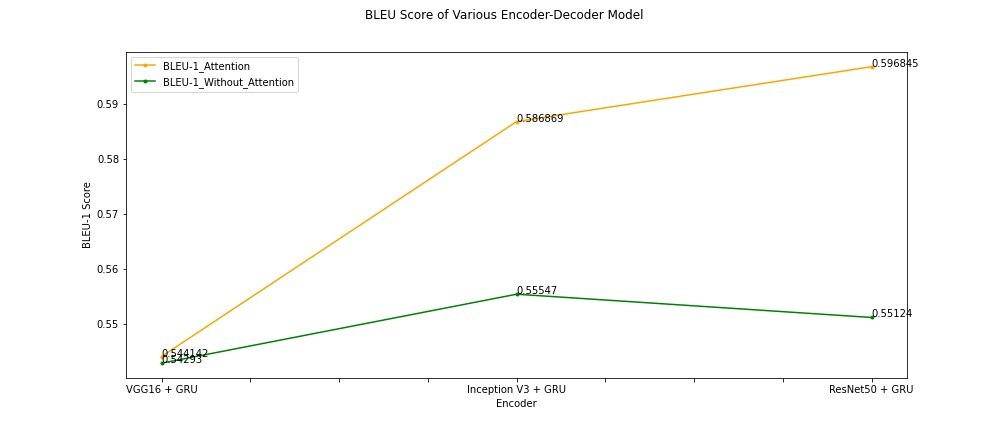
\includegraphics[scale=0.5]{chapters/5/intfig/bleu-1_score_attention.jpg}\hfill
    \caption{Graphical comparision of BLEU-1 score of different encoder-decoder models with and without attention on Flickr8k dataset.}
    \label{img:graph_bleu-1_attention}
\end{figure*}

\noindent The graphical plot \ref{img:graph_bleu-1_attention} demonstrates there is increase in the BLEU-1 score of various encoder-decoder based model using the attention mechanism.

\begin{figure*}[ht!]
    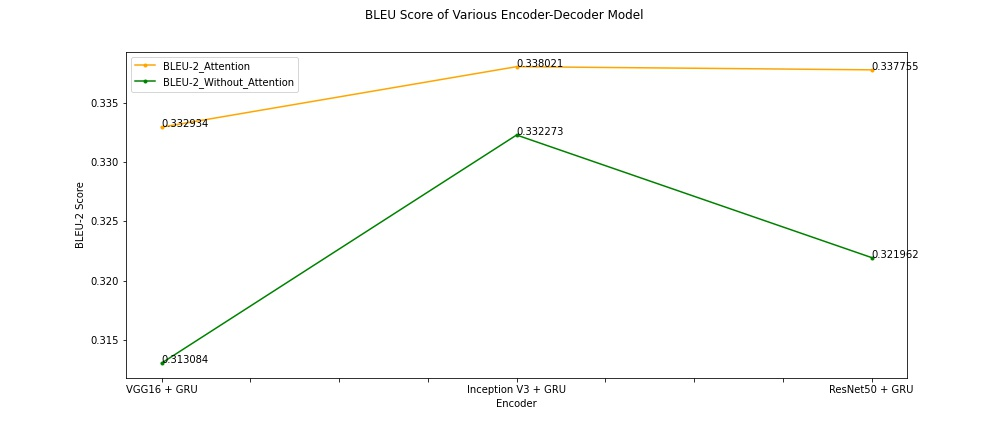
\includegraphics[scale=0.5]{chapters/5/intfig/bleu-2_score_attention.jpg}\hfill
    \caption{Graphical comparision of BLEU-2 score of different encoder-decoder models with and without attention on Flickr8k dataset.}
    \label{img:graph_bleu-2_attention}
\end{figure*}

\noindent The graphical plot \ref{img:graph_bleu-2_attention} demonstrates there is increase in the BLEU-2 score of various encoder-decoder based model using the attention mechanism.

\begin{figure*}[ht!]
    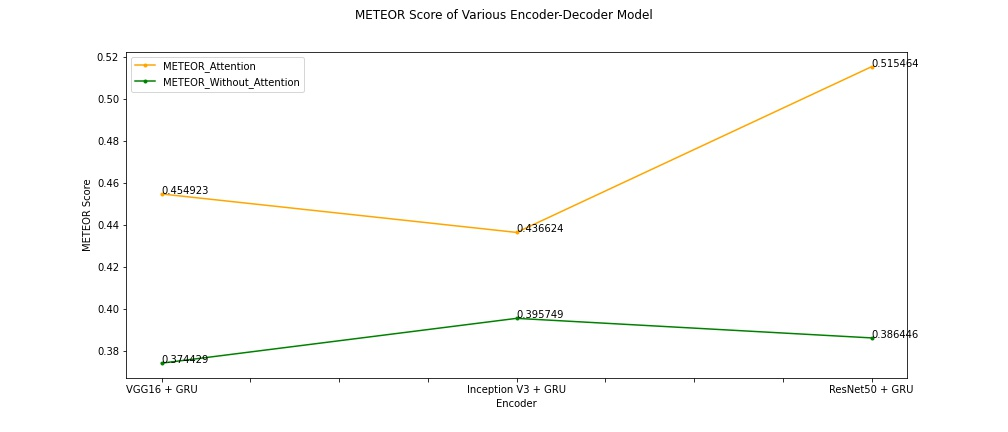
\includegraphics[scale=0.5]{chapters/5/intfig/meteor_score_attention.jpg}\hfill
    \caption{Graphical comparision of METEOR score of different encoder-decoder models with and without attention on Flickr8k dataset.}
    \label{img:meteor_attention}
\end{figure*}

\noindent The graphical plot \ref{img:meteor_attention} demonstrates there is increase in the METEOR score of various encoder-decoder based model using the attention mechanism.

\begin{figure*}[ht!]
    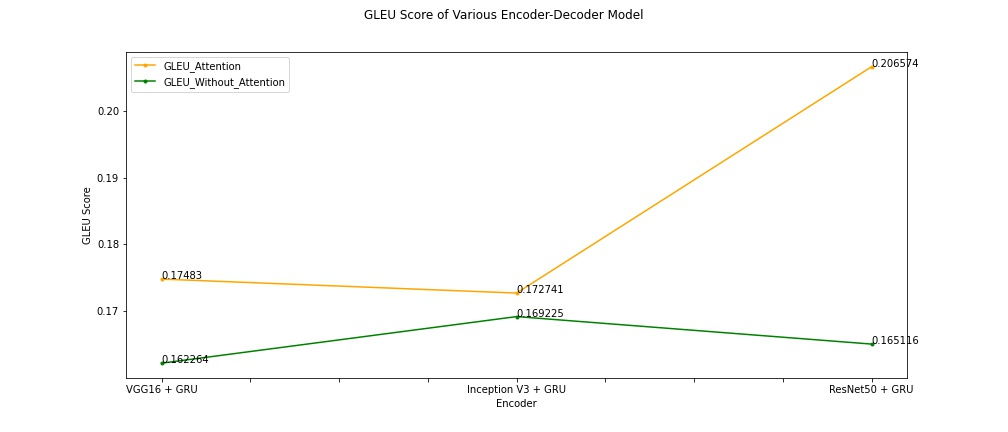
\includegraphics[scale=0.5]{chapters/5/intfig/gleu_score_attention.jpg}\hfill
    \caption{Graphical comparision of GLEU score of different encoder-decoder models with and without attention on Flickr8k dataset.}
    \label{img:gleu_attention}
\end{figure*}

\noindent The graphical plot \ref{img:gleu_attention} demonstrates there is increase in the GLEU score of various encoder-decoder based model using the attention mechanism.

\newpage
\noindent
The above results demonstrates that attention mechanism definitely increased scores of all evaluation metrics: BLEU-1, BLEU-2, METEOR and GLEU. However, there is uncertainty around the selection of encoder. So, we would be deploying all the models with encoder as VGG-16, InceptionV3 and ResNet50. We would automate the process of selection of encoders based on the matching labels achieved from the object detection algorithm.\\ 
\noindent Here, are some screenshots of the generated image descriptions from various encoders with attention.

\begin{figure*}[ht!]
    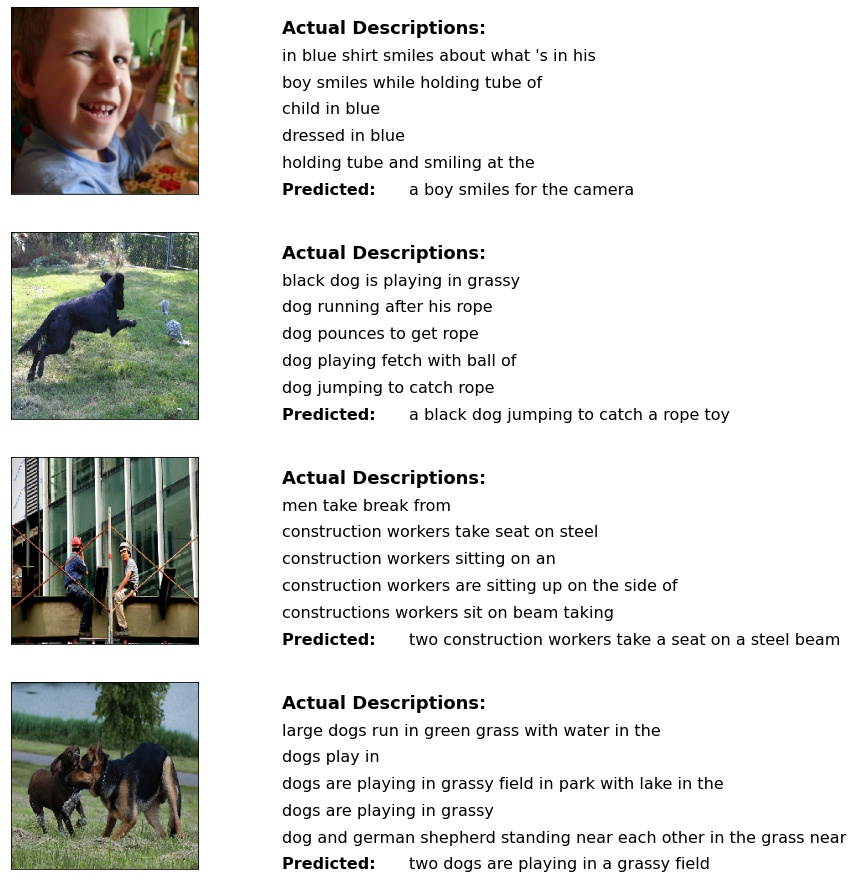
\includegraphics[scale=0.4]{chapters/5/intfig/vgg16_and_gru_with_attention_output.jpg}
    \caption{Sample description of images generated using VGG16 as encoder and GRU as decoder with attention.}
    \label{res:vgg16_gru_attention}
\end{figure*}

\noindent In the Figure \ref{res:vgg16_gru_attention}, the predicted captions are able to identify the object, action and attributes present in the image. The attention mechanism certainly helps in improving the generate captions. When using VGG16 as encoder, generated features are less as compared to InceptionV3 and ResNet50 because of less number of layers to train. \\ \\

\begin{figure*}[ht!]
    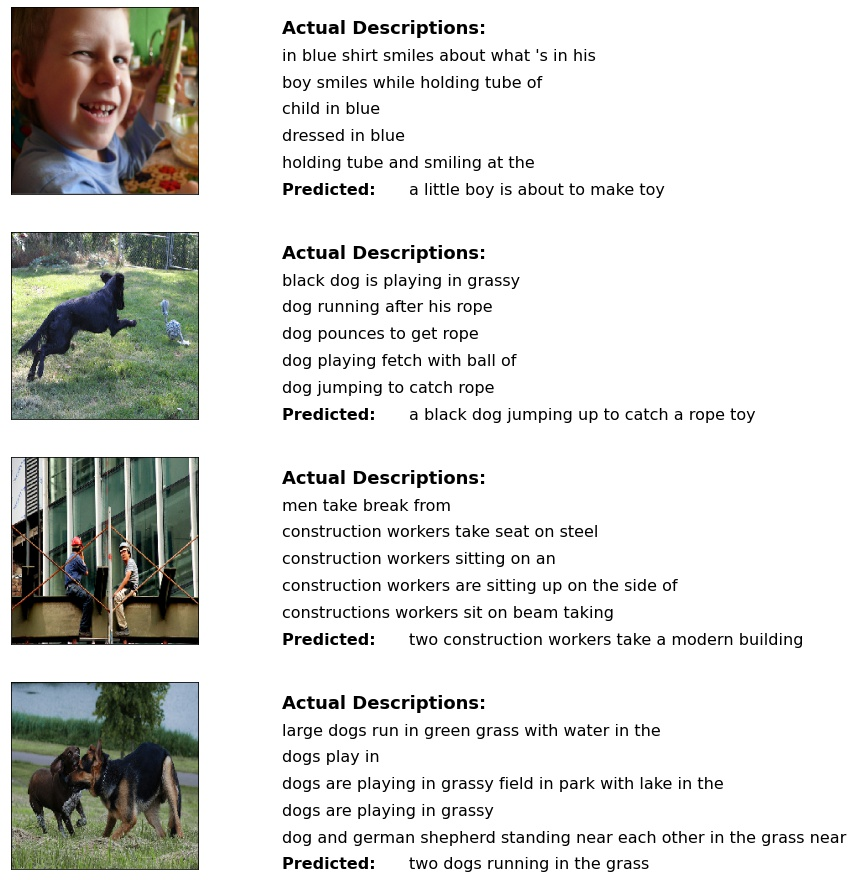
\includegraphics[scale=0.4]{chapters/5/intfig/inception_and_gru_with_attention_output.jpg}
    \caption{Sample description of images generated using Inception V3 as encoder and GRU as decoder with attention.}
    \label{res:inceptionv3_gru_attention}
\end{figure*}

\noindent In the Figure \ref{res:inceptionv3_gru_attention}, the features identified in the images are more as compared to \ref{res:vgg16_gru_attention} because of more number of training layers. But, there are some abnormalities find in the generated in the above architecture as well. This will be solved by automating the selection of encoders.
\newpage
\begin{figure*}[ht!]
    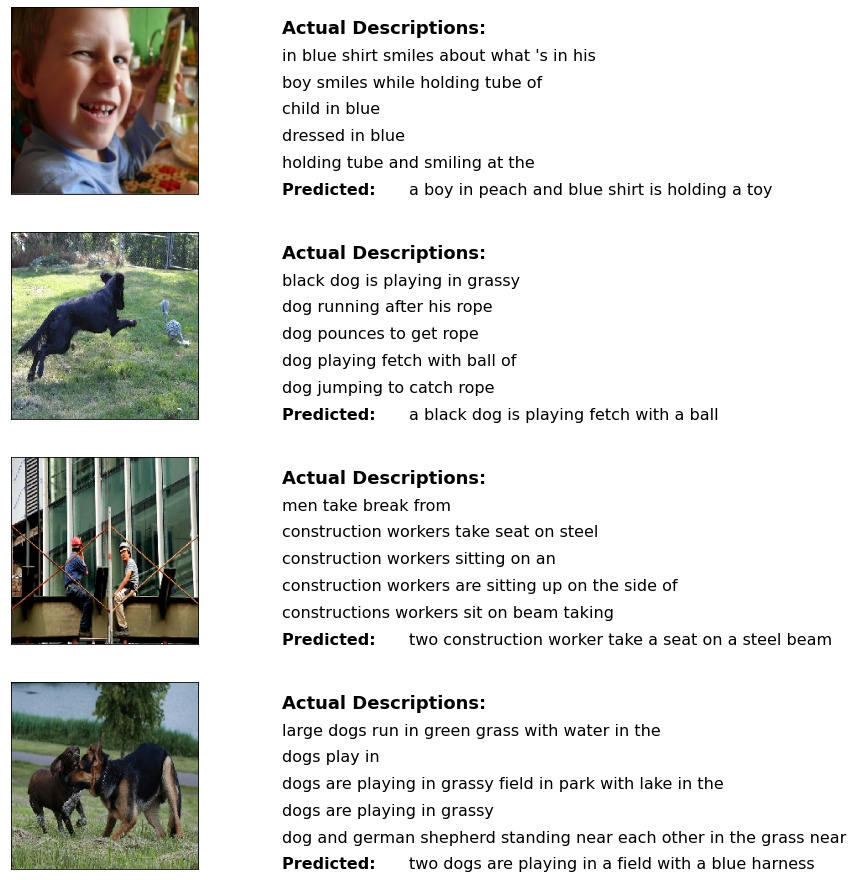
\includegraphics[scale=0.35]{chapters/5/intfig/resnet_and_gru_with_attention_output.jpg}
    \caption{Sample description of images generated using ResNet50 as encoder and GRU as decoder with attention.}
    \label{res:resnet50_gru_attention}
\end{figure*}
\noindent In the Figure \ref{res:resnet50_gru_attention}, the features identified in the images are more as compared to \ref{res:vgg16_gru_attention} and \ref{res:inceptionv3_gru_attention} because of more number of training layers.

\begin{figure*}[ht!]
    \begin{center}
        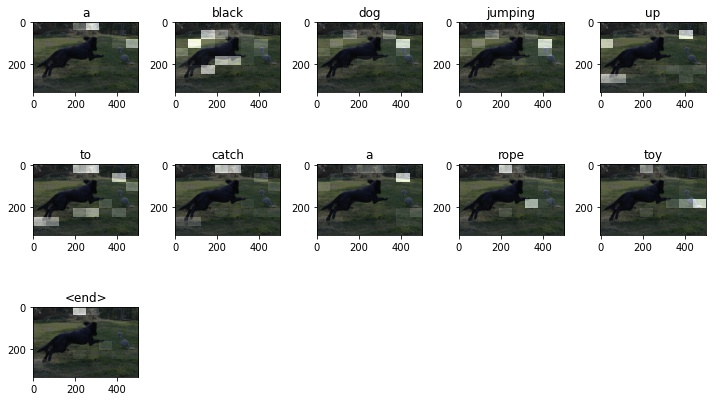
\includegraphics[scale=0.45]{chapters/5/intfig/inception_and_gru_with_attention_plot_attention.jpg}
    \end{center}
    \caption{Sample attention plot for the image description generation}
    \label{res:attention_plot2}
\end{figure*}

\begin{figure*}[ht!]
    \begin{center}
        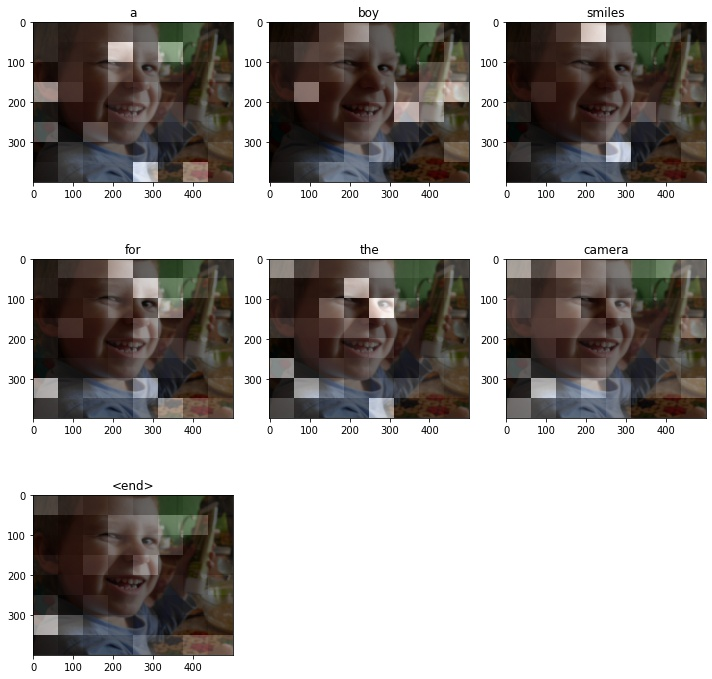
\includegraphics[scale=0.5]{chapters/5/intfig/vgg16_and_gru_with_attention_plot_attention.jpg}
    \end{center}
    \caption{Sample attention plot for the image description generation}
    \label{res:attention_plot}
\end{figure*}

\noindent In the Figure \ref{res:attention_plot2} and \ref{res:attention_plot}, gives the plot of the attention map for each word predicted. The word instead of using the entire image, focuses on certain region of the map which represent that word more accurately.

\noindent To deal with the uncertainty between different encoders and improving the accuracy of the image description, we automated the process
of selection of encoders. For each image, the encoder with
the maximum matching root words with the labels obtained
from label detection algorithm will be considered best. After
experimenting with the automated neural network architecture,
we achieved a BLEU-1 score of \textbf{0.619}. We achieved our goal
of reducing the training time by using GRU decoder and
improving the accuracy by automating the process of selection
of encoders.
\label{chap:intermediate_results}

% \chapter{Future Work}
% \vspace{-1cm}
% \noindent \rule{6.6in}{0.01in}
% \clearpage
\noindent This chapter details the project's conclusion and the thesis's future scope.

\section{Conclusions}
\noindent In this study, we examined the vital challenge of surface floating object detection using the FloW dataset and novel object detection models, particularly GroundedSAM and YOLOv8. In order to automatically annotate images and produce a dataset for training the target model, we made use of the capability of knowledge distillation. We achieved precise and quick floating waste detection by combining the capabilities of GroundedSAM's automatic annotating and YOLOv8's effective real-time detection.
Results showed that our method identified and classified floating waste objects in challenging conditions, including those involving reflections and too much light. The distilled model, developed by transferring knowledge from GroundedSAM to YOLOv8, demonstrated impressive performance, showcasing its potential as a potent tool for practical applications like pollution monitoring, environmental conservation, and search and rescue.

\section{Future Scope}
\noindent A complete analysis of previous methods and approaches used for image description generation has been done in the literature review process.
\begin{enumerate}
    \item Training the final model on the more diverse dataset and leveraging the power of prompt engineering to improve the performance of the model.
    \item Try out various hyperparameter configurations for GroundedSAM and YOLOv8. Various factors, including learning rates, batch sizes, optimizer selections, and regularisation methods.
    \item Find the ideal parameters for efficiently transferring knowledge from GroundedSAM to YOLOv8, extending hyperparameter adjustment to the knowledge distillation procedure.
    \textbf{dont add as bullets, rewrite as whole paragraph and write this in detail}
\end{enumerate}\label{chap:cons_fscope}
%\clearpage
%\mbox{}
%\thispagestyle{empty}
%\newpage
%\addtocounter{page}{-1}
%\appendix
%%%..........................................................................................................................................
%\fancychapter{Appendix}\label{Sunil_Appendix}
%\chapter{Appendix}\label{Sunil_Appendix}
%  
\section{Active Appearance Model}\label{AppendixAAM}
\noindent Active Appearance Model (AAM) \cite{cootes2001active} is a principal component analysis (PCA)-based statistical approach, and it is used to model the variations in shape due to pose, expression, as well as variation in texture due to lighting conditions. So apparently, AAM is a combination of shape model (SM) and appearance/texture model (AM). Learning of AAM model requires a set of training instances having marked with facial landmark points.
\par Fitting of AAM to a given test image {\bf I} is a non-linear optimization problem \cite{baker2004lucas}. The computational complexity of the original active appearance model is of the order of ${\left( {n + m} \right)^2}N$, where $n$ and $m$ denote the number of shape and texture parameters. In general $m >> n$ and thus, the total cost becomes very high, which makes the fitting process very slow. A fast and accurate AAM is proposed in \cite{6751183}, where the total cost is reduced to only few times of $mN$. We employed the same fast-AAM technique in our proposed algorithm (Chapter 4). The objective of fast-AAM is to minimize the mean square error between the model instance and the given test face image over the model parameters. Mathematically, this optimization problem can be expressed as: %equation \ref{eq301}):
\begin{equation}\label{eq301}
{\text{arg }}\mathop {\min }\limits_{{\mathbf{p}}{\text{,}}{\mathbf{c}}} ||{\mathbf{I}}\left( {{\mathbf{W}}\left( {{\mathbf{x}};{\mathbf{p}}} \right)} \right) - {{\mathbf{A}}_0} - {\mathbf{Ac}}||
\end{equation}
where, $\mathbf{p}$ and $\mathbf{c}$ are the parameters of shape and texture models. The symbol $\mathbf{W}$ represents a piece-wise warping function. In Eqn. (\ref{eq301}), $\left\{ {{{\mathbf{A}}_0},{\mathbf{A}} \in {\Re ^{\left\{ {N,m} \right\}}}} \right\}$ defines an appearance model, where ${\mathbf{A}}_0$ is the mean appearance, and $\mathbf{A}$ is a matrix of $m$ eigenvectors corresponding to $m$ largest eigenvalues obtained by applying PCA on shape-free texture training images. The shape-free texture images are obtained by warping each face image so that its landmark points match with the mean shape ${\mathbf{s}}_0$. This process removes spurious texture variations on account of shape differences. Similarly, the shape model ${\text{SM: }}\left\{ {{{\mathbf{s}}_0},{\mathbf{S}} \in {\Re ^{\left\{ {2u,n} \right\}}}} \right\}$ is defined by the mean shape ${\mathbf{s}}_0$ and the transformation matrix $\mathbf{S}$. The columns of $\mathbf{S}$ represent eigenvectors obtained by applying PCA on similarity-free shape instances.
\par Given the models, a test image {\bf I} and its similarity-free shape $\mathbf{s}$, the model parameters can be estimated by using Eqn. (\ref{eq302}) and Eqn. (\ref{eq303}) respectively.
\begin{align}
{\text{  }}{\mathbf{\overset{\lower0.5em\hbox{$\smash{\scriptscriptstyle\frown}$}}{s} }} = {{\mathbf{s}}_0} + {\mathbf{Sp}},{\text{   }}{\mathbf{p}} = {\mathbf{S'}}\left( {{\mathbf{s}} - {{\mathbf{s}}_0}} \right)\label{eq302} \\
{\mathbf{\overset{\lower0.5em\hbox{$\smash{\scriptscriptstyle\frown}$}}{I} }} = {{\mathbf{A}}_0} + {\mathbf{Ac}},{\text{  }}{\mathbf{c}} = {\mathbf{A'}}\left( {{\mathbf{I}} - {{\mathbf{A}}_0}} \right)\label{eq303}
\end{align}
%\begin{equation}\label{eq303}
%{\mathbf{\overset{\lower0.5em\hbox{$\smash{\scriptscriptstyle\frown}$}}{I} }} = {{\mathbf{A}}_0} + {\mathbf{Ac}},{\text{  }}{\mathbf{c}} = {\mathbf{A'}}\left( {{\mathbf{I}} - {{\mathbf{A}}_0}} \right)
%\end{equation}
The optimum values of $\mathbf{p}$ and $\mathbf{c}$ can be obtained by the method proposed in \cite {6751183}. 
\section{Uncorrelated Discriminant Locality Preserving Projection Analysis (UDLPP)}\label{AppendixUDLPP}
\noindent The UDLPP \cite{yu2008uncorrelated} seeks for a transformation matrix ${\mathbf{V}}$, which projects samples of high-dimensional data onto a low dimensional space such that it preserves the topology of intra-class samples of the observation space. Additionally, it also maximizes between-class-scatter-matrix of the reduced sample space. The above criterion is formulated as a minimization problem which is represented as follows:
\begin{equation}\label{ICVGIP-eqn-1}
{J_{UDLPP}}\left( {\mathbf{V}} \right) = \frac{{{J_1}\left( {\mathbf{V}} \right)}}{{{J_2}\left( {\mathbf{V}} \right)}} = \frac{{tr\left( {{{\mathbf{V}}^T}{\mathbf{XL}}{{\mathbf{X}}^T}{\mathbf{V}}} \right)}}{{tr\left( {{{\mathbf{V}}^T}{\mathbf{XB}}{{\mathbf{X}}^T}{\mathbf{V}}} \right)}}
\end{equation} 
The numerator term ${J_1}\left( {\mathbf{V}} \right) = tr\left( {{{\mathbf{V}}^T}{\mathbf{XL}}{{\mathbf{X}}^T}{\mathbf{V}}} \right)$ of Eqn. (\ref{ICVGIP-eqn-1}) reflects the sum of the distances between the samples of the intra-class in the reduced subspace \cite{eleftheriadis2015discriminative}. In Eqn. (\ref{ICVGIP-eqn-1}), $tr\left(  \cdot  \right)$ represents the trace of a matrix, the $N \times N$ matrix ${\mathbf{L}}$ is known as Laplacian matrix. The Laplacian matrix, ${\mathbf{L}}$, is defined as ${\mathbf{L}} = {\mathbf{D}} - {\mathbf{A}}$, where ${{\mathbf{D}}_{ii}} = \sum\nolimits_j {{{\mathbf{A}}_{ij}}} $, and similarity matrix ${\mathbf{A}}$ is obtained by applying RBF kernel which is given as:
\begin{equation}\label{ICVGIP-eqn-2}
{{\mathbf{A}}_{ij}} = \left\{ {\begin{array}{*{20}{lc}}
  {\exp \left( { - \frac{{||{{\mathbf{x}}_i} - {{\mathbf{x}}_j}|{|^2}}}{{\sigma}^2 }} \right)} \\ 
  {0{\text{,     otherwise}}} 
\end{array}} \right.{\text{, if }}{c_i} = {c_j}{\text{ }}
\end{equation}
where, $\sigma$ represents width of the kernel function and ${c_i}$ indicates the class of the $i^{th}$ sample of the observation space. On the other hand, denominator term of the Eqn. (\ref{ICVGIP-eqn-1}) {\em i.e.,} ${J_2}\left( {\mathbf{V}} \right) = tr\left( {{{\mathbf{V}}^T}{\mathbf{XB}}{{\mathbf{X}}^T}{\mathbf{V}}} \right)$ represents sum of distances of all pairs of distinct classes, and hence ${J_2}\left( {\mathbf{V}} \right)$ has to be maximized for any classification problem. Furthermore, a statistical constraint has been imposed on Eqn. (\ref{ICVGIP-eqn-1}), so that any two components of the reduced feature vector become uncorrelated. The two feature components $y_i$ and $y_j$ ($i\ne j$) of extracted feature vector ${\mathbf{y}} = {{\mathbf{V}}^T}{\mathbf{x}}$ are said to be uncorrelated iff 
\begin{equation}\label{ICVGIP-eqn-3}
E\left[ {\left( {{y_i} - E\left( {{y_i}} \right)} \right)\left( {{y_j} - E\left( {{y_j}} \right)} \right)} \right] = 0
\end{equation}
Hence, the final minimization problem of UDLPP becomes a constraint optimization problem which is further converted to the generalized eigenvalue problem. The eigenvectors corresponding to $d$ smallest eigenvalues represent the first $d$-columns of the required transformation matrix.

%\clearpage
%%..........................................................................................................................................
%\fancychapter{Cepstral Analysis}
%\label{app:lpc}
%\include{chapters/Appendix/CFA}
%\clearpage
%%..........................................................................................................................................
%\fancychapter{Linear Prediction Coefficients Computation}
%\label{app:sine}
%\include{chapters/Appendix/Appendix_lpc_V2}
%\clearpage
%%..........................................................................................................................................
%\fancychapter{Composite Objective Quality Measures}
%\label{app:cqm}
%\include{Chapters/Appendix/Appendix_cqm_V1}
%\clearpage
%%..........................................................................................................................................
%\fancychapter{MFCC Feature Extraction}
%\label{app:mfcc}
%\include{Chapters/Appendix/Appendix_mfcc_V1}
%\clearpage
%%..........................................................................................................................................
%\fancychapter{Gaussian Mixture Models}
%\label{app:gmm}
%\include{Chapters/Appendix/Appendix_gmm_V1}
%\clearpage
%..........................................................................................................................................
%\doublespacing
%\normalsize
%\pdfbookmark{Publications}{Publications}
%\fancyhead[LE]{\bfseries\small{List of Publications}}
%\fancyhead[RO]{\bfseries\small{List of Publications}}
%\pdfbookmark[1]{List of Publications}{los}
%\addstarredchapter{List of Publications}
%%\newpage
\begin{center}
{\LARGE \bf LIST OF PUBLICATIONS}
\end{center}
\vspace{0.2in}

\renewcommand{\labelenumi}{\arabic{enumi}.}   % Added on 09/08/2008
\renewcommand{\theenumii}{\arabic{enumii}}
\renewcommand{\labelenumii}{\theenumii}
%\noindent{\large \bf \textit{LIST OF PUBLICATIONS}} \\
%\vspace{0.2cm}
\noindent{\bf{Journal Publications}}
\begin{enumerate}
	\item {\label{IET2016}} {\bf Sunil Kumar}, M.K. Bhuyan and B. K. Chakraborty, ``Extraction of informative regions of a face for facial expression recognition", \emph{IET Computer Vision}, vol. 10, no. 6, pp. 567-576, 2016.
	
	\item {\label{JMUI2016}} {\bf Sunil Kumar}, M.K. Bhuyan and B. K. Chakraborty, ``Extraction of Texture and Geometrical Features from Informative Facial Regions for Sign Language Recognition", \emph{Journal on Multimodal User Interfaces, Springer}, pp. 1-13, 2017.
	
\end{enumerate}
\noindent{\bf Manuscripts under Review}
\begin{enumerate}
	\item {\label{CSVT2017}} {\bf Sunil Kumar} and M.K. Bhuyan ``Multilevel Uncorrelated Discriminative Shared Gaussian Process for Multiview Facial Expression Recognition", \emph{IEEE Transactions on Circuits Systems Video Technology}, {\bfseries{(Date of communication : 03-Nov-2016)}}.
	
	\item  {\label{AC2017}} {\bf Sunil Kumar} and M.K. Bhuyan ``Hierarchical Uncorrelated Multiview Discriminant Locality Preserving Projection for Multiview Facial Expression Recognition", \emph{IET Biometrics}, {\bfseries{(To be communicated)}}.
	
\end{enumerate}
\noindent{\bf {Conference Publications}}
\begin{enumerate}
	
	\item {\label{ICVGIP2016}} {\bf Sunil Kumar}, M.K. Bhuyan, and Biplab Ketan Chakraborty, ``Uncorrelated multiview discriminant locality preserving projection analysis for multiview facial expression recognition", \emph{Proceedings of Tenth Indian Conference on Computer Vision, Graphics and Image Processing (ICVGIP 2016).} ACM, 2016.
	
	\item {\label{NCC2016}} {\bf Sunil Kumar}, M.K. Bhuyan and B. K. Chakraborty, ``An efficient face model for facial expression recognition", \emph{Proceedings of Twenty Second National Conference on Communication (NCC 2016), Guwahati.} pp. 1-6, 2016.
	
	\item {\label{RAICS2015}} {\bf Sunil Kumar}, and M.K. Bhuyan. ``Neutral expression modeling in feature domain for facial expression recognition", \emph{Proceedings of IEEE conference on Recent Advances in Intelligent Computational Systems (RAICS 2015)}, pp. 224-228, 2015.
	
\end{enumerate}

%\noindent{\bf{Refereed Journals:}}
%\begin{enumerate}
%\item {\label{IET2016}} Sunil Kumar, M. K. Bhuyan and B. K. Chakraborty, ``Extraction of informative regions of a face for facial expression recognition", \emph{in IET Computer Vision}, vol. 10, no. 6, pp. 567-576, 9 2016.
%\end{enumerate}
%
%\item  {\label{JMUI2016}} Sunil Kumar, M. K. Bhuyan and B. K. Chakraborty, ``Extraction of Texture and Geometrical Features from Informative Facial Regions for Sign Language Recognition", \emph{Journal on Multimodal User Interfaces, Springer}, 2016.
%
%\noindent{\bf Manuscripts under Review}
%\begin{enumerate}
%\item {\label{CSVT2017}} Sunil Kumar, M. K. Bhuyan and Akhil Babu Manam, ``Multilevel Uncorrelated Discriminative Shared Gaussian Process for Multiview Facial Expression Recognition", \emph{IEEE Transactions on Circuits Systems Video Technology}, 2016.
%	
%\item {\label{AC2017}} Sunil Kumar, M. K. Bhuyan, B. K. Chakraborty and Yuji Iwahori ``Hierarchical Uncorrelated Multiview Discriminant Locality Preserving Projection for Multiview Facial Expression Recognition", \emph{IEEE Transactions on Affective Computing}, 2016.
%	
%\end{enumerate}
%\noindent{\bf {Refereed Conferences:}}
%\begin{enumerate}
%
%\item {\label{ICVGIP2016}} Sunil Kumar, M. K. Bhuyan, and Biplab Ketan Chakraborty, ``Uncorrelated multiview discriminant locality preserving projection analysis for multiview facial expression recognition", \emph{Proceedings of the Tenth Indian Conference on Computer Vision, Graphics and Image Processing.} ACM, 2016.
%
%\item {\label{NCC2016}} Sunil Kumar, M. K. Bhuyan and B. K. Chakraborty, ``An efficient face model for facial expression recognition", \emph{2016 Twenty Second National Conference on Communication (NCC), Guwahati.} pp. 1-6, 2016.
%
%\item {\label{RAICS2015}} Sunil Kumar, and M. K. Bhuyan. ``Neutral expression modeling in feature domain for facial expression recognition", \emph{Intelligent Computational Systems (RAICS), 2015 IEEE Recent Advances in. IEEE}, 2015.
%
%\end{enumerate}

%\clearpage

%% LIST OF SYMBOLS
%\fancyhead[LE]{\bfseries\small{List of Symbols}}
%\fancyhead[RO]{\bfseries\small{List of Symbols}}
%\pdfbookmark[1]{List of Symbols}{los}
%\addstarredchapter{List of Symbols}
%\chapter*{List of Symbols}

\begin{longtable}{ll}

%A

$D$                 & Dimension of the observation space \\
$d$                 & Dimension of the reduced subspace \\
$A_k$               & Similarity matrix of $k^{th}$ view \\
$\mathbf{I}$        & Identity matrix\\
$U$                 & Uniformity \\
$C$                 & Number of classes \\
$\lambda$           & Number of facial sub-regions \\
$\dim \left(  \cdot  \right)$ & Dimension of argument \\
$C$                 & Number of classes \\
$ \bot $            & Perpendicular symbol \\ 
$\beta$             & Precision parameter \\
${\gamma ^v}$       & Back-projection parameter\\
$R\left( {\mathbf{A}} \right)$  & regularization term \\
$I_{bp}$            & Independent back-projection \\
$S_{bp}$            & Single back-projection \\
${n_c^v}$           & Number of samples belongs to $c^{th}$ \\
${\mathbf{S}}_{lb}^v$ & Local between-class scatter matrix for $v^{th}$ view \\
${{\mathbf{L}}_{net}}$ & Sum of normalize Laplacian matrices for all the views \\
${{{\mathbf{S}}_b}}$ & Between-class scatter matrix \\
${{{\mathbf{S}}_w}}$ & Within-class scatter matrix \\
${{\delta _{i,j}}}$ & Kronecker delta function \\
${\bm{\theta }} = \left\{ {{{\bm{\theta }}_1},{{\bm{\theta }}_2}, \cdots ,{{\bm{\theta }}_V}} \right\}$   & Kernel parameters of the shared observation space \\
${\mathbf{X}}^v$     & Observation space for $v^{th}$ view \\
${{\mathbf{Y}}_{ccs}}$ & Reduced correlated common space \\
${{\mathbf{Y}}_{ucs}}$ & Reduced uncorrelated common space \\
${{\mathbf{Q}}_{eq}}$ & Intra and inter-views transformation matrix \\
${{\mathbf{Q}}_{kk}}$ & Intra-view local between-class scatter matrix \\
${{\mathbf{Q}}_{kl}}$ & Inter-view local between-class scatter matrix \\
${{\mathbf{P}}_{eq}}$ & Intra and inter-views LPP transformation matrix \\
${{\mathbf{L}}_{kl}}$ & Inter-view Laplacian matrix \\
${{\mathbf{L}}_{ccs}}$ & Laplacian matrix for CCS \\
${{\mathbf{B}}_{ccs}}$ & Local between-class scatter matrix for CCS \\


\end{longtable}

%\clearpage
%******************************************************************************************************************************************************************

%**************************************************BIBLIOGRAPHY********************************************************
\fancyhead[LE]{\bfseries\small{Bibliography}}
\fancyhead[RO]{\bfseries\small{Bibliography}}
\pdfbookmark[1]{Bibliography}{los}
\addstarredchapter{Bibliography}   % PKM 05/07/08 (For more options refer minitoc.pdf on page 36)
\baselineskip 14pt   %12, 18 and 24
\small
\bibliographystyle{IEEEtran}
\bibliographystyle{unsrt}
\bibliography{chapters/references/MyBibliography_database_Maninder}
%\clearpage
%**************************************************PUBLICATIONS****************************************************************************************************************



\end{document}
